\documentclass[11pt,a4paper]{book}
\usepackage[italian]{babel}
\usepackage[T1]{fontenc}
\usepackage[utf8]{inputenc}
\usepackage{lmodern}
\usepackage{geometry}
\geometry{margin=2.5cm}
\usepackage{graphicx}
\usepackage{xcolor}
\usepackage{listings}
\usepackage{amsmath,amssymb}
\usepackage{booktabs}
\usepackage{hyperref}
\usepackage{float}
\usepackage{enumitem}

\lstdefinestyle{python}{
  language=Python,
  basicstyle=\ttfamily\small,
  keywordstyle=\color{blue!70!black},
  commentstyle=\color{green!40!black},
  stringstyle=\color{red!60!black},
  numbers=left,
  numberstyle=\tiny,
  numbersep=8pt,
  frame=single,
  breaklines=true,
  showstringspaces=false,
  tabsize=4,
  backgroundcolor=\color{green!5}
}
\lstset{style=python}

\lstdefinestyle{output}{
    basicstyle=\ttfamily\small,
    showstringspaces=false,
    frame=single,
    breaklines=true,
    columns=fullflexible,
    keepspaces=true,
    backgroundcolor=\color{blue!5}
}


\title{Costruire figure scientifiche con Python\\
Un percorso graduale con NumPy, Matplotlib e SciPy}
\author{Giuseppe Mandaglio}
\date{}

\begin{document}
\maketitle
\tableofcontents

\chapter{Introduzione}
Questo documento illustra, attraverso una sequenza di script di complessità crescente, come costruire una figura scientifica in Python. Si parte da un grafico essenziale e si introducono progressivamente marker, legenda, etichette degli assi, più serie di dati, salvataggio su file, barre di errore e personalizzazione grafica avanzata. L'ultimo capitolo è dedicato al fit parabolico, confrontando l'approccio specializzato di NumPy con quello più generale di SciPy.

I pacchetti utilizzati sono:
\begin{itemize}
  \item \texttt{NumPy}, per la lettura e la manipolazione numerica dei dati;
  \item \texttt{Matplotlib}, per la costruzione delle figure;
  \item \texttt{SciPy}, per il fit di funzioni definite dall'utente.
\end{itemize}


\section{Le liste in Python}

Le liste, indicate in Python con il tipo \texttt{list}, rappresentano una delle strutture dati più utilizzate del linguaggio. Una lista è una sequenza ordinata e modificabile di oggetti. Può crescere o ridursi durante l'esecuzione del programma e, a differenza degli array tradizionali del C++, può contenere elementi di tipo differente.

\subsection{Creazione di una lista}

Una lista vuota può essere creata mediante una coppia di parentesi quadre:

\begin{lstlisting}[style=python]
pino = []
\end{lstlisting}

In alternativa, si può utilizzare il costruttore \texttt{list()}:

\begin{lstlisting}[style=python]
pino = list()
\end{lstlisting}

È possibile aggiungere un elemento alla fine della lista mediante il metodo \texttt{append()}:

\begin{lstlisting}[style=python]
pino = []
pino.append(1)
pino.append(2)
pino.append(3)

print(pino)
\end{lstlisting}

L'output è:

\begin{lstlisting}[style=python, numbers=none]
[1, 2, 3]
\end{lstlisting}

Il metodo \texttt{append()} aggiunge un solo oggetto alla volta. L'oggetto può essere un numero, una stringa, un'altra lista o, più in generale, qualunque oggetto Python.

\subsection{Iterazione sugli elementi}

Le liste sono oggetti iterabili. È quindi possibile percorrerne gli elementi con un ciclo \texttt{for}:

\begin{lstlisting}[style=python]
for a in pino:
    print(a)
\end{lstlisting}

L'output è:

\begin{lstlisting}[style=output, numbers=none]
1
2
3
\end{lstlisting}

A ogni iterazione, la variabile \texttt{a} assume il valore dell'elemento successivo della lista. Non è necessario utilizzare esplicitamente gli indici quando interessa soltanto il valore degli elementi.

Se servono sia l'indice sia il valore, si può usare \texttt{enumerate()}:

\begin{lstlisting}[style=python]
for indice, valore in enumerate(pino):
    print(indice, valore)
\end{lstlisting}
fornendo il risultato:
\begin{lstlisting}[style=output, numbers=none]
0 1
1 2
2 3
\end{lstlisting}
la funzione \textbf{enumerate()} funziona su qualunque iterabile, ad esempio su una stringa:
\begin{lstlisting}[style=python]
frutto = "banana"
for a,b in enumerate(frutto):
    print(a,b)
\end{lstlisting}
ottenendo:
\begin{lstlisting}[style=output, numbers=none]
0 b
1 a
2 n
3 a
4 n
5 a
\end{lstlisting}
\subsection{Liste eterogenee}

Una lista Python può contenere oggetti di tipo diverso:

\begin{lstlisting}[style=python]
pino.append("ciao")
print(pino)
\end{lstlisting}

L'output diventa:

\begin{lstlisting}[style=python, numbers=none]
[1, 2, 3, 'ciao']
\end{lstlisting}

Il ciclo \texttt{for} continua a funzionare normalmente:

\begin{lstlisting}[style=python]
for a in pino:
    print(a)
\end{lstlisting}

ottenendo:

\begin{lstlisting}[style=python, numbers=none]
1
2
3
ciao
\end{lstlisting}

Questa flessibilità è utile per collezioni generiche, ma rende le liste meno efficienti degli array NumPy nel calcolo numerico intensivo.

\subsection{Operazioni sulle liste}

Date due liste:

\begin{lstlisting}[style=python]
pino = [1, 2, 3, "ciao"]
pina = [1.2, 3.2, 3.4]
\end{lstlisting}

l'operatore \texttt{+} produce una nuova lista ottenuta concatenando le due liste:

\begin{lstlisting}[style=python]
risultato = pino + pina
print(risultato)
\end{lstlisting}

Output:

\begin{lstlisting}[style=python, numbers=none]
[1, 2, 3, 'ciao', 1.2, 3.2, 3.4]
\end{lstlisting}

L'operatore \texttt{+} non esegue una somma elemento per elemento. Questo comportamento è diverso da quello degli array NumPy.

Se vogliamo effettuare una somma vettoriale di due liste, supponendo che le liste abbiano la stessa dimensione e contengano solo numeri reali, allora possimo utilizzare il seguente codice che in modo elegante e pythonesco usando la funzione \textbf{zip} e grazie ad essa ciclare su due indici contemporaneamente:
\begin{lstlisting}[style=python, numbers=none]
a = [1, 2, 3]
b = [4, 5, 6]

c = [x + y for x, y in zip(a, b)]

print(c)
# [5, 7, 9]
\end{lstlisting}

Oltre al concatenamento esistono altre funzioni che possono essere utilizzate con le liste. Ad esempio la moltiplicazione della lista:
\begin{lstlisting}[style=python, numbers=none]
a = [1, 2]

print(a * 3)
# [1, 2, 1, 2, 1, 2]

#oppure molto utile nelle inizializzazioni
lista = [0] * 10
#[0, 0, 0, 0, 0, 0, 0 ,0 ,0 ,0]
\end{lstlisting}

\subsection{Indicizzazione positiva e negativa}

Gli elementi di una lista sono identificati da indici interi. La numerazione parte da zero:

\begin{lstlisting}[style=python]
pino = [10, 20, 30, 40, 50]
\end{lstlisting}

\begin{center}
\begin{tabular}{c|ccccc}
\toprule
Elemento & 10 & 20 & 30 & 40 & 50 \\
\midrule
Indice & 0 & 1 & 2 & 3 & 4 \\
\bottomrule
\end{tabular}
\end{center}

Per esempio:

\begin{lstlisting}[style=python]
print(pino[0])
print(pino[3])
\end{lstlisting}

produce:

\begin{lstlisting}[style=python, numbers=none]
10
40
\end{lstlisting}

Se si usa un indice esterno all'intervallo valido, Python genera un'eccezione \texttt{IndexError}:

\begin{lstlisting}[style=python]
print(pino[10])
\end{lstlisting}


Python permette di contare gli elementi partendo dalla fine della sequenza. L'ultimo elemento ha indice \texttt{-1}, il penultimo ha indice \texttt{-2} e così via:

\begin{center}
\begin{tabular}{c|ccccc}
\toprule
Elemento & 10 & 20 & 30 & 40 & 50 \\
\midrule
Indice positivo & 0 & 1 & 2 & 3 & 4 \\
Indice negativo & -5 & -4 & -3 & -2 & -1 \\
\bottomrule
\end{tabular}
\end{center}

Per esempio:

\begin{lstlisting}[style=python]
print(pino[-1])
print(pino[-2])
\end{lstlisting}

produce:

\begin{lstlisting}[style=python, numbers=none]
50
40
\end{lstlisting}

L'indicizzazione negativa è utile quando si vuole accedere agli ultimi elementi senza conoscere esplicitamente la lunghezza della lista.

\subsection{Lo slicing}

Lo \emph{slicing} permette di estrarre una porzione di una sequenza. La sintassi generale è:

\begin{lstlisting}[style=python, numbers=none]
lista[inizio:fine]
\end{lstlisting}

L'indice \texttt{inizio} è incluso, mentre l'indice \texttt{fine} è escluso. Per esempio:

\begin{lstlisting}[style=python]
pino = [10, 20, 30, 40, 50]
parte = pino[1:4]
print(parte)
\end{lstlisting}

produce:

\begin{lstlisting}[style=python, numbers=none]
[20, 30, 40]
\end{lstlisting}

Sono stati selezionati gli elementi con indici \texttt{1}, \texttt{2} e \texttt{3}. L'elemento con indice \texttt{4} non è incluso.

\subsection{Omissione degli estremi nello slicing}

Se si omette l'indice iniziale, lo slicing parte dall'inizio della lista:

\begin{lstlisting}[style=python]
print(pino[:3])
\end{lstlisting}

Output:

\begin{lstlisting}[style=python, numbers=none]
[10, 20, 30]
\end{lstlisting}

Se si omette l'indice finale, lo slicing continua fino alla fine:

\begin{lstlisting}[style=python]
print(pino[2:])
\end{lstlisting}

Output:

\begin{lstlisting}[style=python, numbers=none]
[30, 40, 50]
\end{lstlisting}

La scrittura

\begin{lstlisting}[style=python]
copia = pino[:]
\end{lstlisting}

Seleziona tutti gli elementi e crea una nuova lista. Come si vedrà successivamente, questa è una copia superficiale.

\subsection{Il passo dello slicing}

La forma completa dello slicing è:

\begin{lstlisting}[style=python, numbers=none]
lista[inizio:fine:passo]
\end{lstlisting}

Il parametro \texttt{passo} indica ogni quanti elementi effettuare la selezione:

\begin{lstlisting}[style=python]
numeri = [0, 1, 2, 3, 4, 5, 6, 7, 8, 9]
print(numeri[0:10:2])
\end{lstlisting}

Output:

\begin{lstlisting}[style=python, numbers=none]
[0, 2, 4, 6, 8]
\end{lstlisting}

Il passo può anche essere negativo. Un uso frequente è l'inversione dell'ordine degli elementi:

\begin{lstlisting}[style=python]
print(numeri[::-1])
\end{lstlisting}

Output:

\begin{lstlisting}[style=python, numbers=none]
[9, 8, 7, 6, 5, 4, 3, 2, 1, 0]
\end{lstlisting}

Un passo uguale a zero non è ammesso e produce un'eccezione.

\subsection{Slicing e indici negativi}

Lo slicing può essere combinato con l'indicizzazione negativa:

\begin{lstlisting}[style=python]
pino = [10, 20, 30, 40, 50]

print(pino[-3:])
print(pino[:-2])
\end{lstlisting}

Output:

\begin{lstlisting}[style=python, numbers=none]
[30, 40, 50]
[10, 20, 30]
\end{lstlisting}

Nel primo caso vengono selezionati gli ultimi tre elementi. Nel secondo caso vengono selezionati tutti gli elementi tranne gli ultimi due.

\subsection{Modifica degli elementi e dello slicing}

Le liste sono modificabili, cioè sono oggetti \emph{mutabili}:

\begin{lstlisting}[style=python]
pino = [1, 2, 3]
pino[1] = 100
print(pino)
\end{lstlisting}

Output:

\begin{lstlisting}[style=python, numbers=none]
[1, 100, 3]
\end{lstlisting}

È possibile modificare anche una porzione della lista:

\begin{lstlisting}[style=python]
pino = [1, 2, 3, 4, 5]
pino[1:4] = [20, 30, 40]
print(pino)
\end{lstlisting}

Output:

\begin{lstlisting}[style=python, numbers=none]
[1, 20, 30, 40, 5]
\end{lstlisting}

Nell'assegnazione a uno slicing, il numero di elementi inseriti non deve necessariamente coincidere con il numero di elementi sostituiti. La lunghezza della lista può quindi cambiare.

\subsection{La funzione range}

La funzione \texttt{range()} produce una sequenza di interi, spesso utilizzata nei cicli. Non restituisce direttamente una lista:

\begin{lstlisting}[style=python]
cino = range(20)
print(cino)
\end{lstlisting}

Output:

\begin{lstlisting}[style=python, numbers=none]
range(0, 20)
\end{lstlisting}

Gli elementi sono comunque indicizzabili:

\begin{lstlisting}[style=python]
print(cino[0])
print(cino[4])
print(cino[19])
\end{lstlisting}

Per ottenere una vera lista si può scrivere:

\begin{lstlisting}[style=python]
cino = list(range(20))
\end{lstlisting}

La forma generale è \texttt{range(inizio, fine, passo)}. Anche in questo caso l'estremo finale è escluso.

\subsection{Principali metodi delle liste}

\begin{center}
\renewcommand{\arraystretch}{1.2}
\begin{tabular}{>{\ttfamily}l p{9cm}}
\toprule
\normalfont Metodo & Descrizione \\
\midrule
append(x) & Aggiunge \texttt{x} alla fine della lista. \\
insert(i, x) & Inserisce \texttt{x} nella posizione \texttt{i}. \\
extend(L) & Aggiunge alla lista tutti gli elementi dell'iterabile \texttt{L}. \\
remove(x) & Elimina la prima occorrenza dell'elemento \texttt{x}. \\
pop() & Elimina e restituisce l'ultimo elemento. \\
pop(i) & Elimina e restituisce l'elemento con indice \texttt{i}. \\
clear() & Rimuove tutti gli elementi. \\
copy() & Crea una copia superficiale della lista. \\
count(x) & Conta le occorrenze di \texttt{x}. \\
index(x) & Restituisce l'indice della prima occorrenza di \texttt{x}. \\
sort() & Ordina la lista sul posto. \\
reverse() & Inverte sul posto l'ordine degli elementi. \\
\bottomrule
\end{tabular}
\end{center}

\subsection{Ordinamento}

Se gli elementi sono confrontabili tra loro, il metodo \texttt{sort()} ordina la lista sul posto:

\begin{lstlisting}[style=python]
gino = [2, 4, 1]
gino.sort()
print(gino)
\end{lstlisting}

Output:

\begin{lstlisting}[style=python, numbers=none]
[1, 2, 4]
\end{lstlisting}

Anche una lista di numeri in virgola mobile può essere ordinata:

\begin{lstlisting}[style=python]
pina = [1.2, 3.2, 3.4]
pina.sort()
\end{lstlisting}

Una lista contenente tipi non confrontabili genera invece un errore:

\begin{lstlisting}[style=python]
pino = [1, 2, 3, "ciao"]
pino.sort()
\end{lstlisting}

Python non può stabilire un ordinamento tra un numero intero e una stringa. Il risultato è un \texttt{TypeError}.

La funzione \texttt{sorted()}, diversamente dal metodo \texttt{sort()}, restituisce una nuova lista senza modificare quella originale:

\begin{lstlisting}[style=python]
gino = [2, 4, 1]
ordinata = sorted(gino)
\end{lstlisting}

\subsection{Assegnazione e riferimenti}

In Python le variabili contengono riferimenti agli oggetti. Consideriamo:

\begin{lstlisting}[style=python]
a = [1, 2, 3]
b = a
\end{lstlisting}

L'assegnazione \texttt{b = a} non crea una nuova lista. Le variabili \texttt{a} e \texttt{b} fanno riferimento allo stesso oggetto. Di conseguenza:

\begin{lstlisting}[style=python]
b[0] = 100

print(a)
print(b)
\end{lstlisting}

produce:

\begin{lstlisting}[style=python, numbers=none]
[100, 2, 3]
[100, 2, 3]
\end{lstlisting}

È possibile verificare l'identità degli oggetti mediante l'operatore \texttt{is}:

\begin{lstlisting}[style=python]
print(a is b)
\end{lstlisting}

Il risultato è \texttt{True}.

\subsection{Copia superficiale: shallow copy}

Per creare un nuovo contenitore si può utilizzare il metodo \texttt{copy()}:

\begin{lstlisting}[style=python]
a = [1, 2, 3]
b = a.copy()

b[0] = 100

print(a)
print(b)
\end{lstlisting}

Output:

\begin{lstlisting}[style=python, numbers=none]
[1, 2, 3]
[100, 2, 3]
\end{lstlisting}

La stessa copia superficiale può essere ottenuta mediante:

\begin{lstlisting}[style=python]
b = a[:]
b = list(a)
\end{lstlisting}

Per una lista semplice, contenente oggetti immutabili come numeri o stringhe, una copia superficiale è normalmente sufficiente.

\subsection{Il problema delle liste annidate}

Consideriamo una lista contenente altre liste:

\begin{lstlisting}[style=python]
a = [[1, 2], [3, 4]]
b = a.copy()
\end{lstlisting}

Il contenitore esterno è stato copiato, ma le liste interne sono ancora condivise. Pertanto:

\begin{lstlisting}[style=python]
b[0][0] = 999

print(a)
print(b)
\end{lstlisting}

produce:

\begin{lstlisting}[style=python, numbers=none]
[[999, 2], [3, 4]]
[[999, 2], [3, 4]]
\end{lstlisting}

La copia è detta \emph{superficiale} perché duplica soltanto il contenitore più esterno. Gli oggetti mutabili contenuti al suo interno restano condivisi.

È importante distinguere tra la sostituzione di una lista interna e la modifica di una lista interna:

\begin{lstlisting}[style=python]
a = [[1, 2], [3, 4]]
b = a.copy()

b[0] = [100, 200]
\end{lstlisting}

In questo caso viene sostituito soltanto il riferimento presente in \texttt{b}; la prima lista interna di \texttt{a} non viene modificata.

\subsection{Copia profonda: deep copy}

Quando è necessario duplicare ricorsivamente anche gli oggetti contenuti, si usa la funzione \texttt{deepcopy()} del modulo \texttt{copy}:

\begin{lstlisting}[style=python]
import copy

a = [[1, 2], [3, 4]]
b = copy.deepcopy(a)

b[0][0] = 999

print(a)
print(b)
\end{lstlisting}

Output:

\begin{lstlisting}[style=python, numbers=none]
[[1, 2], [3, 4]]
[[999, 2], [3, 4]]
\end{lstlisting}

La copia profonda crea una struttura indipendente anche ai livelli interni. È utile quando una struttura contiene oggetti mutabili annidati e si vuole evitare qualsiasi condivisione involontaria.

\subsection{List comprehension}

Una \emph{list comprehension} permette di costruire una lista in modo compatto:

\begin{lstlisting}[style=python]
quadrati = [x**2 for x in range(10)]
print(quadrati)
\end{lstlisting}

Output:

\begin{lstlisting}[style=python, numbers=none]
[0, 1, 4, 9, 16, 25, 36, 49, 64, 81]
\end{lstlisting}

È possibile aggiungere una condizione:

\begin{lstlisting}[style=python]
quadrati_pari = [x**2 for x in range(10) if x % 2 == 0]
\end{lstlisting}

Le list comprehension sono adatte a trasformazioni compatte e leggibili. Quando la logica diventa complessa, un ciclo tradizionale può risultare più chiaro.

\section{Lettura di file testuali senza NumPy}

Nei primi programmi Python può essere utile leggere un file di dati senza utilizzare NumPy, rappresentando il contenuto mediante una \textbf{lista di liste}. Ogni riga del file diventa una sottolista.

Supponiamo che il file \texttt{datuzzi.txt} contenga:

\begin{lstlisting}[style=output]
1.0 2.3 4.5
2.0 3.1 5.0
3.0 4.2 6.7
\end{lstlisting}

\subsection{Prima versione: lista di liste di stringhe}

Il metodo più elegante consiste nell'utilizzare direttamente il file come iteratore.

\begin{lstlisting}[style=python]
dati = []

with open("datuzzi.txt") as f:
    for riga in f:
        valori = riga.split()
        dati.append(valori)

print(dati)
\end{lstlisting}

L'istruzione \texttt{split()} divide la riga nelle sue colonne utilizzando gli spazi come separatori.

L'output sarà:

\begin{lstlisting}[style=output]
[['1.0', '2.3', '4.5'],
 ['2.0', '3.1', '5.0'],
 ['3.0', '4.2', '6.7']]
\end{lstlisting}

Osserviamo che tutti gli elementi sono ancora stringhe.

\subsection{Seconda versione: lista di liste di numeri reali}

Spesso si desidera ottenere direttamente dei numeri utilizzabili nei calcoli. È sufficiente convertire ogni elemento mediante \texttt{float()}.

\begin{lstlisting}[style=python]
dati = []

with open("datuzzi.txt") as f:
    for riga in f:
        valori = [float(x) for x in riga.split()]
        dati.append(valori)

print(dati)
\end{lstlisting}

L'output diventa:

\begin{lstlisting}[style=output]
[[1.0, 2.3, 4.5],
 [2.0, 3.1, 5.0],
 [3.0, 4.2, 6.7]]
\end{lstlisting}

Ora ogni riga è una lista di numeri reali.

\subsection{Analisi dettagliata del codice}

La prima istruzione

\begin{lstlisting}[style=python]
dati = []
\end{lstlisting}

crea una lista vuota che conterrà tutte le righe del file.

L'istruzione

\begin{lstlisting}[style=python]
with open("datuzzi.txt") as f:
\end{lstlisting}

apre il file in lettura e associa l'oggetto file alla variabile \texttt{f}. Il costrutto \texttt{with} garantisce inoltre la chiusura automatica del file al termine del blocco.

Successivamente troviamo

\begin{lstlisting}[style=python]
for riga in f:
\end{lstlisting}

che legge una riga del file a ogni iterazione.

Infine:

\begin{lstlisting}[style=python]
valori = [float(x) for x in riga.split()]
\end{lstlisting}

esegue due operazioni:

\begin{enumerate}
    \item divide la riga nelle varie colonne mediante \texttt{split()};
    \item converte ciascuna colonna in un numero reale mediante \texttt{float()}.
\end{enumerate}

Ad esempio, se

\begin{lstlisting}[style=python]
riga = "1.0 2.3 4.5\n"
\end{lstlisting}

allora

\begin{lstlisting}[style=python]
riga.split()
\end{lstlisting}

produce

\begin{lstlisting}[style=output]
['1.0', '2.3', '4.5']
\end{lstlisting}

mentre

\begin{lstlisting}[style=python]
[float(x) for x in riga.split()]
\end{lstlisting}

produce

\begin{lstlisting}[style=output]
[1.0, 2.3, 4.5]
\end{lstlisting}

La sintassi precedente prende il nome di \textbf{list comprehension} ed equivale a:

\begin{lstlisting}[style=python]
valori = []

for x in riga.split():
    valori.append(float(x))
\end{lstlisting}

Infine

\begin{lstlisting}[style=python]
dati.append(valori)
\end{lstlisting}

aggiunge la riga appena letta alla lista principale.

\subsection{Perché non compare il metodo \texttt{read()}?}

Molti studenti si aspettano di trovare una chiamata del tipo

\begin{lstlisting}[style=python]
contenuto = f.read()
\end{lstlisting}

ma nel codice precedente non è necessaria.

Il motivo è che un oggetto file in Python è \textbf{iterabile}. Ciò significa che può essere utilizzato direttamente in un ciclo \texttt{for}.

Quando scriviamo

\begin{lstlisting}[style=python]
for riga in f:
\end{lstlisting}

Python legge automaticamente una riga alla volta fino alla fine del file.

Dal punto di vista concettuale il comportamento è simile a:

\begin{lstlisting}[style=python]
while True:
    riga = f.readline()

    if riga == "":
        break

    # elaborazione della riga
\end{lstlisting}

ma con una sintassi molto più compatta.

\subsection{Differenza tra \texttt{read()} e iterazione}

Con \texttt{read()} si legge l'intero file in una sola volta:

\begin{lstlisting}[style=python]
with open("datuzzi.txt") as f:
    contenuto = f.read()
\end{lstlisting}

Se il file contiene:

\begin{lstlisting}[style=output]
1 2 3
4 5 6
7 8 9
\end{lstlisting}

allora la variabile \texttt{contenuto} vale:

\begin{lstlisting}[style=output]
"1 2 3\n4 5 6\n7 8 9\n"
\end{lstlisting}

Successivamente sarebbe necessario separare le righe:

\begin{lstlisting}[style=python]
for riga in contenuto.splitlines():
    ...
\end{lstlisting}

L'approccio basato sull'iteratore

\begin{lstlisting}[style=python]
for riga in f:
\end{lstlisting}

è invece più naturale, più leggibile e più efficiente, poiché legge una sola riga alla volta e non richiede di caricare l'intero file in memoria.

\subsection{Accesso agli elementi}

Alla fine del programma, la struttura dati è una lista di liste:

\begin{lstlisting}[style=output]
[
 [1.0, 2.3, 4.5],
 [2.0, 3.1, 5.0],
 [3.0, 4.2, 6.7]
]
\end{lstlisting}

Possiamo quindi accedere agli elementi usando due indici.

\begin{lstlisting}[style=python]
dati[0]
\end{lstlisting}

restituisce la prima riga:

\begin{lstlisting}[style=output]
[1.0, 2.3, 4.5]
\end{lstlisting}

mentre

\begin{lstlisting}[style=python]
dati[0][1]
\end{lstlisting}

restituisce il secondo valore della prima riga:

\begin{lstlisting}[style=output]
2.3
\end{lstlisting}

In questo modo una semplice lista di liste può rappresentare una tabella numerica senza ricorrere a NumPy.


\section{Array NumPy e confronto con gli array C++}

Le liste Python sono estremamente flessibili, ma non sono progettate specificamente per il calcolo numerico intensivo. In ambito scientifico si utilizzano frequentemente gli array della libreria NumPy.

\subsection{Creazione di un array NumPy}

Per utilizzare NumPy si importa normalmente la libreria con l'abbreviazione \texttt{np}:

\begin{lstlisting}[style=python]
import numpy as np

x = np.array([1, 2, 3, 4])
print(x)
\end{lstlisting}

Output:

\begin{lstlisting}[style=python, numbers=none]
[1 2 3 4]
\end{lstlisting}

Un array NumPy è un oggetto di tipo \texttt{ndarray}.

\subsection{Tipo uniforme degli elementi}

Gli elementi di un array NumPy condividono normalmente lo stesso tipo, indicato dall'attributo \texttt{dtype}:

\begin{lstlisting}[style=python]
x = np.array([1, 2, 3])
y = np.array([1.0, 2.0, 3.0])

print(x.dtype)
print(y.dtype)
\end{lstlisting}

Questa uniformità consente una rappresentazione compatta dei dati e operazioni numeriche efficienti.

Se si mescolano interi e numeri in virgola mobile, NumPy sceglie un tipo comune capace di rappresentare gli elementi:

\begin{lstlisting}[style=python]
x = np.array([1, 2.5, 3])
print(x)
print(x.dtype)
\end{lstlisting}

Gli interi vengono convertiti in numeri in virgola mobile.

\subsection{Dimensione, forma e numero di elementi}

Gli attributi principali sono:

\begin{itemize}
    \item \texttt{ndim}: numero di dimensioni;
    \item \texttt{shape}: forma dell'array;
    \item \texttt{size}: numero complessivo di elementi;
    \item \texttt{dtype}: tipo degli elementi.
\end{itemize}

Esempio bidimensionale:

\begin{lstlisting}[style=python]
a = np.array([[1, 2, 3],
              [4, 5, 6]])

print(a.ndim)
print(a.shape)
print(a.size)
print(a.dtype)
\end{lstlisting}

La forma \texttt{(2, 3)} indica due righe e tre colonne.

\subsection{Creazione rapida di array}

NumPy fornisce diverse funzioni per creare array:

\begin{lstlisting}[style=python]
a = np.zeros(5)
b = np.ones(5)
c = np.arange(0, 10, 2)
d = np.linspace(0.0, 1.0, 6)
\end{lstlisting}

La funzione \texttt{arange()} è simile a \texttt{range()}, ma restituisce un array NumPy. La funzione \texttt{linspace()} genera invece un numero stabilito di valori equidistanti, includendo normalmente entrambi gli estremi.

\subsection{Operazioni vettoriali}

Una caratteristica fondamentale degli array NumPy è la possibilità di applicare un'operazione a tutti gli elementi senza scrivere esplicitamente un ciclo:

\begin{lstlisting}[style=python]
x = np.array([1, 2, 3])

print(x + 1)
print(x * 2)
print(x**2)
\end{lstlisting}

Output:

\begin{lstlisting}[style=python, numbers=none]
[2 3 4]
[2 4 6]
[1 4 9]
\end{lstlisting}

Queste operazioni sono dette vettorializzate.

\subsection{Differenza tra liste e array nelle operazioni}

Con due liste Python, l'operatore \texttt{+} esegue una concatenazione:

\begin{lstlisting}[style=python]
a = [1, 2, 3]
b = [10, 20, 30]
print(a + b)
\end{lstlisting}

Output:

\begin{lstlisting}[style=python, numbers=none]
[1, 2, 3, 10, 20, 30]
\end{lstlisting}

Con due array NumPy, lo stesso operatore esegue una somma elemento per elemento:

\begin{lstlisting}[style=python]
a = np.array([1, 2, 3])
b = np.array([10, 20, 30])
print(a + b)
\end{lstlisting}

Output:

\begin{lstlisting}[style=python, numbers=none]
[11 22 33]
\end{lstlisting}

Gli array devono avere forme compatibili. NumPy può estendere automaticamente array di forme differenti secondo le regole del \emph{broadcasting}.

\subsection{Indicizzazione e slicing negli array NumPy}

Gli array monodimensionali usano indicizzazione positiva, negativa e slicing in modo simile alle liste:

\begin{lstlisting}[style=python]
x = np.array([10, 20, 30, 40, 50])

print(x[0])
print(x[-1])
print(x[1:4])
print(x[::2])
\end{lstlisting}

Per gli array multidimensionali si separano gli indici con una virgola:

\begin{lstlisting}[style=python]
a = np.array([[1, 2, 3],
              [4, 5, 6],
              [7, 8, 9]])

print(a[1, 2])
print(a[:, 1])
print(a[0:2, 1:3])
\end{lstlisting}

L'espressione \texttt{a[1, 2]} seleziona l'elemento della riga con indice 1 e della colonna con indice 2. Il simbolo \texttt{:} seleziona tutti gli elementi lungo una dimensione.

\subsection{Maschere booleane}

Una condizione applicata a un array produce un array di valori booleani:

\begin{lstlisting}[style=python]
x = np.array([3, 7, 2, 8, 1])
maschera = x > 4

print(maschera)
print(x[maschera])
\end{lstlisting}

Output:

\begin{lstlisting}[style=python, numbers=none]
[False  True False  True False]
[7 8]
\end{lstlisting}

Una maschera può essere usata anche per modificare simultaneamente gli elementi selezionati:

\begin{lstlisting}[style=python]
errori = np.array([0.2, 0.0, 0.5, 0.0])
errori[errori == 0] = 1
print(errori)
\end{lstlisting}

Tutti gli elementi uguali a zero vengono sostituiti con uno.

\subsection{View e copy in NumPy}

Una differenza importante rispetto alle liste è che lo slicing di un array NumPy restituisce normalmente una \emph{view}, cioè una vista sugli stessi dati:

\begin{lstlisting}[style=python]
x = np.array([1, 2, 3, 4])
y = x[1:3]

y[0] = 100

print(x)
print(y)
\end{lstlisting}

Output:

\begin{lstlisting}[style=python, numbers=none]
[  1 100   3   4]
[100   3]
\end{lstlisting}

La modifica di \texttt{y} ha modificato anche \texttt{x}, perché i due array condividono gli stessi dati sottostanti.

Per ottenere un array indipendente si deve richiedere esplicitamente una copia:

\begin{lstlisting}[style=python]
x = np.array([1, 2, 3, 4])
y = x[1:3].copy()

y[0] = 100

print(x)
print(y)
\end{lstlisting}

In questo caso \texttt{x} non viene modificato.

\subsection{Funzioni statistiche e riduzioni}

NumPy fornisce funzioni che operano sull'intero array:

\begin{lstlisting}[style=python]
x = np.array([1.0, 2.0, 3.0, 4.0])

print(np.sum(x))
print(np.mean(x))
print(np.std(x))
print(np.min(x))
print(np.max(x))
\end{lstlisting}

Negli array multidimensionali si può specificare l'asse lungo il quale effettuare l'operazione:

\begin{lstlisting}[style=python]
a = np.array([[1, 2, 3],
              [4, 5, 6]])

print(np.sum(a, axis=0))
print(np.sum(a, axis=1))
\end{lstlisting}

Con \texttt{axis=0} si riducono le righe e si ottiene un risultato per ogni colonna. Con \texttt{axis=1} si riducono le colonne e si ottiene un risultato per ogni riga.

\subsection{Array tradizionali del C++}

In C++ un array tradizionale può essere dichiarato nel modo seguente:

\begin{lstlisting}[style=c++]
int a[5] = {1, 2, 3, 4, 5};
\end{lstlisting}

Le sue caratteristiche principali sono:

\begin{itemize}
    \item la dimensione è fissata;
    \item tutti gli elementi hanno lo stesso tipo;
    \item non esiste un metodo equivalente a \texttt{append()};
    \item l'array non conserva autonomamente l'informazione sulla propria lunghezza quando viene passato a una funzione come puntatore;
    \item l'accesso fuori dai limiti non viene normalmente controllato durante l'esecuzione.
\end{itemize}

Per esempio:

\begin{lstlisting}[style=c++]
int a[5] = {1, 2, 3, 4, 5};
a[100] = 3;
\end{lstlisting}

L'accesso è fuori dai limiti dell'array e produce comportamento indefinito. Il programma potrebbe arrestarsi, corrompere memoria o sembrare funzionare.

\subsection{La copia degli array tradizionali in C++}

Gli array tradizionali non possono essere copiati direttamente mediante una semplice assegnazione:

\begin{lstlisting}[style=c++]
int a[3] = {1, 2, 3};
int b[3];

// b = a;  // non consentito per gli array tradizionali
\end{lstlisting}

Gli elementi devono essere copiati singolarmente o mediante funzioni e algoritmi appropriati:

\begin{lstlisting}[style=c++]
for (int i = 0; i < 3; ++i) {
    b[i] = a[i];
}
\end{lstlisting}

\subsection{std::array: array moderno a dimensione fissa}

Il contenitore \texttt{std::array}, disponibile nel C++ moderno, rappresenta un array a dimensione fissa con un'interfaccia più sicura e completa:

\begin{lstlisting}[style=c++]
#include <array>

std::array<int, 3> a = {1, 2, 3};
std::array<int, 3> b = a;
\end{lstlisting}

A differenza dell'array tradizionale, \texttt{std::array} può essere copiato direttamente. La dimensione resta comunque fissata a compile time.

Il metodo \texttt{at()} controlla i limiti:

\begin{lstlisting}[style=c++]
int valore = a.at(2);
\end{lstlisting}

Se l'indice non è valido, viene generata un'eccezione. L'operatore \texttt{[]} non effettua invece necessariamente tale controllo.

\subsection{std::vector: contenitore dinamico del C++}

Il contenitore C++ più vicino, per alcuni aspetti, a una lista Python è \texttt{std::vector}:

\begin{lstlisting}[style=c++]
#include <vector>

std::vector<int> v;

v.push_back(1);
v.push_back(2);
v.push_back(3);
\end{lstlisting}

Il metodo \texttt{push\_back()} svolge un ruolo simile a \texttt{append()}. Tuttavia, tutti gli elementi di uno \texttt{std::vector<int>} devono essere di tipo \texttt{int}.

La copia di un vettore crea un nuovo contenitore con una copia degli elementi:

\begin{lstlisting}[style=c++]
std::vector<int> a = {1, 2, 3};
std::vector<int> b = a;

b[0] = 100;
\end{lstlisting}

La modifica di \texttt{b} non modifica \texttt{a}.

\subsection{Limiti del parallelismo tra Python e C++}

Non esiste una corrispondenza perfetta tra le strutture considerate:

\begin{itemize}
    \item una lista Python è dinamica, mutabile e può contenere tipi diversi;
    \item un array NumPy contiene dati omogenei ed è progettato per operazioni numeriche vettorializzate;
    \item un array tradizionale C++ ha dimensione fissa e offre un controllo di basso livello;
    \item \texttt{std::array} è un contenitore moderno a dimensione fissa;
    \item \texttt{std::vector} è dinamico, ma resta omogeneo rispetto al tipo degli elementi.
\end{itemize}

NumPy non è semplicemente una versione Python di \texttt{std::vector}: offre array multidimensionali, broadcasting, maschere booleane e operazioni vettorializzate.

\subsection{Confronto riassuntivo}

\begin{center}
\small
\renewcommand{\arraystretch}{1.25}
\begin{tabular}{p{3.5cm}cccc}
\toprule
Caratteristica & Lista Python & NumPy & Array C++ & \texttt{std::vector} \\
\midrule
Dimensione dinamica & Sì & Non normalmente & No & Sì \\
Tipi eterogenei & Sì & No & No & No \\
Indicizzazione negativa & Sì & Sì & No & No \\
Slicing nativo & Sì & Sì & No & No \\
Operazioni vettoriali & No & Sì & No & No \\
Maschere booleane & No & Sì & No & No \\
Controllo automatico con \texttt{[]} & Sì & Sì & No & No \\
Copia con assegnazione & Riferimento & Copia/view secondo l'operazione & Non consentita & Copia \\
Prestazioni numeriche & Limitate & Elevate & Elevate & Elevate \\
\bottomrule
\end{tabular}
\end{center}

La voce ``copia con assegnazione'' richiede attenzione: per una lista Python, \texttt{b = a} crea un nuovo riferimento allo stesso oggetto; per uno \texttt{std::vector}, \texttt{b = a} copia gli elementi; in NumPy il comportamento dipende dall'operazione utilizzata e lo slicing crea normalmente una vista.

\subsection{Regole pratiche}

\begin{itemize}
    \item Usare le \textbf{liste Python} per collezioni generiche, dinamiche e potenzialmente eterogenee.
    \item Usare gli \textbf{array NumPy} per dati numerici, analisi scientifica, algebra lineare, istogrammi e operazioni vettorializzate.
    \item Usare \textbf{\texttt{std::array}} in C++ quando la dimensione è nota e fissa.
    \item Usare \textbf{\texttt{std::vector}} in C++ quando serve un contenitore dinamico e omogeneo.
    \item Verificare sempre se un'operazione crea un nuovo oggetto, un nuovo riferimento oppure una vista dei dati esistenti.
\end{itemize}


\section{Struttura dei file di dati}
Il file \texttt{datios.txt} contiene quattro colonne:
\[
 x,\qquad y,\qquad \sigma_x,\qquad \sigma_y,
\]
dove $\sigma_x$ e $\sigma_y$ rappresentano le incertezze associate alle due coordinate. Il file \texttt{Kter.txt} contiene invece tre colonne:
\[
 x,\qquad y_1,\qquad y_2.
\]
Negli script originali il secondo file è indicato come \texttt{Kter2.dat}; nel presente documento si usa \texttt{Kter.txt}, cioè il nome del file effettivamente disponibile.

\chapter{Dal grafico minimo alla figura completa}

\section{Il grafico più semplice: \texttt{plot\_bad.py}}
\begin{lstlisting}
import numpy as np
import matplotlib.pyplot as plt

dati = np.loadtxt("datios.txt")
x = dati[:, 0]
y = dati[:, 1]
plt.plot(x, y)
plt.show()
\end{lstlisting}

\subsection*{Spiegazione delle istruzioni}
\begin{description}[style=nextline]
  \item[\texttt{import numpy as np}] Importa NumPy e assegna al modulo l'abbreviazione convenzionale \texttt{np}.
  \item[\texttt{import matplotlib.pyplot as plt}] Importa l'interfaccia procedurale di Matplotlib con l'abbreviazione \texttt{plt}.
  \item[\texttt{np.loadtxt("datios.txt")}] Legge il file testuale e costruisce un array bidimensionale. Ogni riga del file diventa una riga dell'array e ogni colonna del file diventa una colonna dell'array.
  \item[\texttt{dati[:, 0]}] Il simbolo \texttt{:} seleziona tutte le righe, mentre \texttt{0} seleziona la prima colonna. Il risultato viene assegnato a \texttt{x}.
  \item[\texttt{dati[:, 1]}] Seleziona la seconda colonna e la assegna a \texttt{y}.
  \item[\texttt{plt.plot(x, y)}] Disegna $y$ in funzione di $x$. In assenza di opzioni, Matplotlib collega i punti mediante una linea continua.
  \item[\texttt{plt.show()}] Visualizza la figura in una finestra grafica oppure nel backend utilizzato dall'ambiente di lavoro.
\end{description}

Questo primo script è sufficiente per verificare rapidamente l'andamento dei dati, ma la figura non contiene marker, legenda, nomi degli assi o unità di misura.

\begin{figure}[H]
\centering
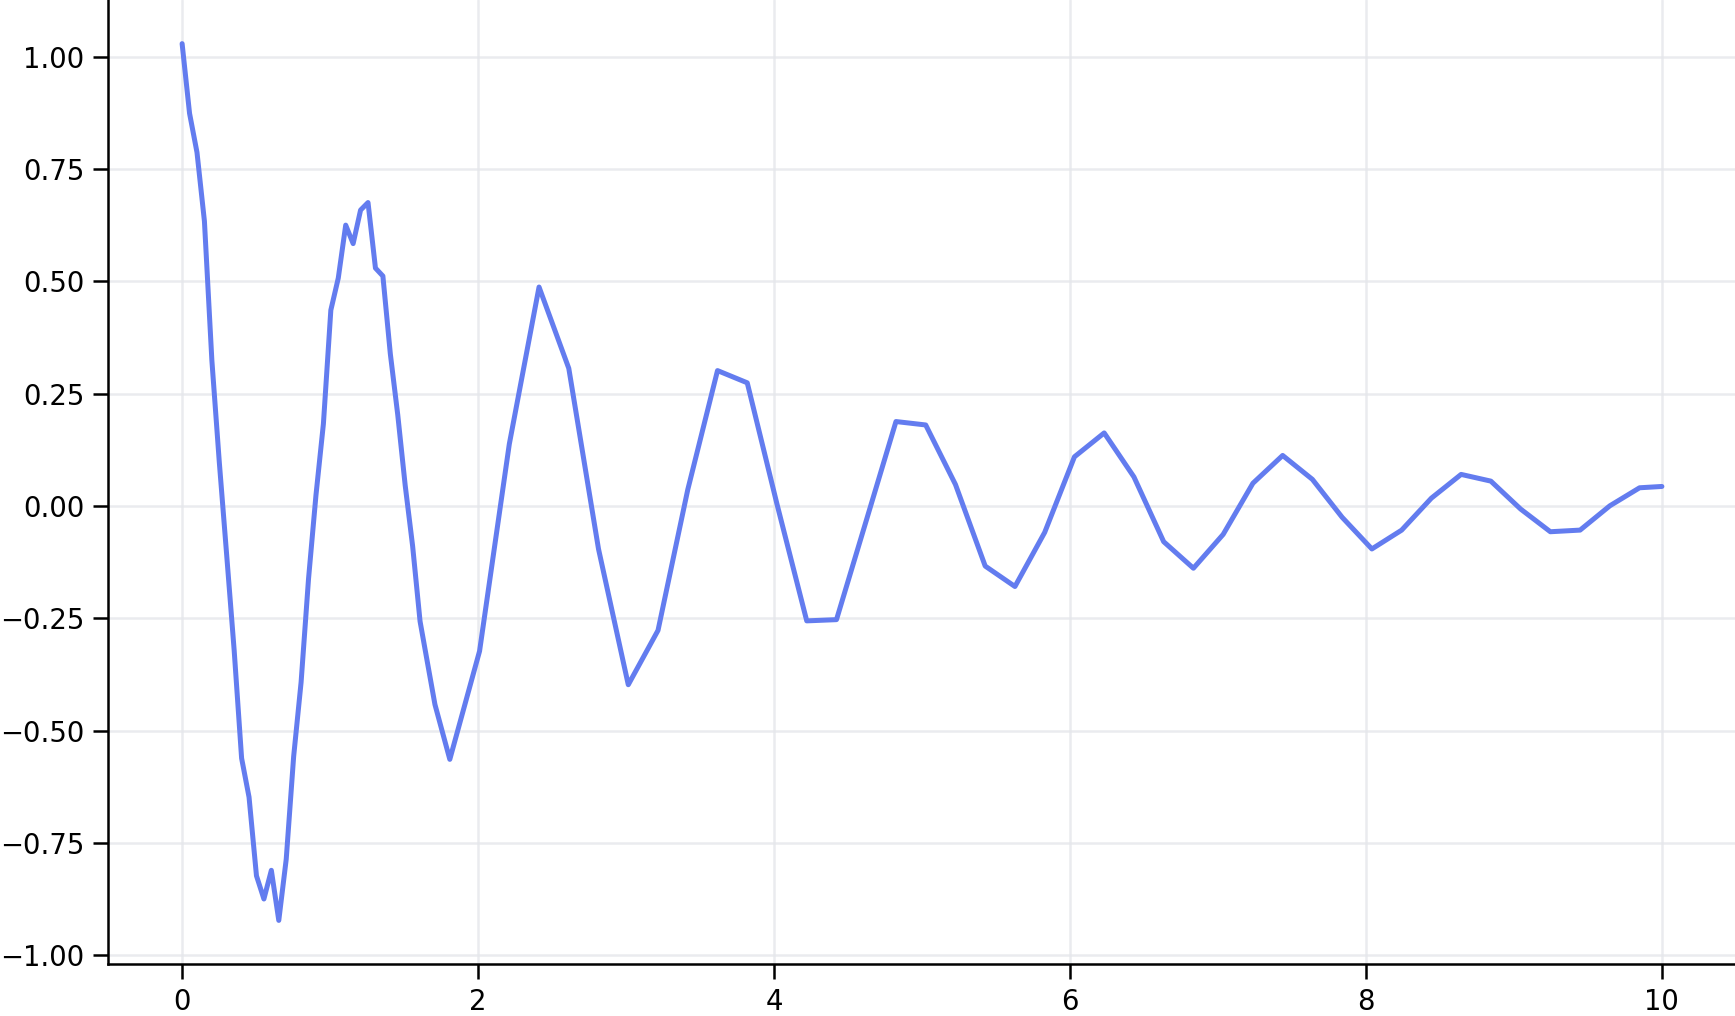
\includegraphics[width=.78\textwidth]{fig_plot_bad.png}
\caption{Risultato prodotto da \texttt{plot\_bad.py}.}
\end{figure}

\section{Rappresentare punti separati: \texttt{plot\_bad2.py}}
\begin{lstlisting}
import numpy as np
import matplotlib.pyplot as plt

dati = np.loadtxt("datios.txt")
x = dati[:, 0]
y = dati[:, 1]
plt.plot(x, y, "o")
plt.show()
\end{lstlisting}

La sola differenza rispetto allo script precedente è la stringa di formato \texttt{"o"}. Essa richiede marker circolari. Poiché non viene specificato uno stile di linea, i punti non sono collegati. Questa rappresentazione è più adatta quando si vogliono mostrare misure discrete senza suggerire che tra due punti consecutivi sia stata osservata una linea continua.

La stringa di formato può combinare colore, marker e stile della linea. Per esempio, \texttt{"ro-"} indica cerchi rossi collegati da una linea continua. È tuttavia spesso più leggibile usare argomenti espliciti, come \texttt{marker="o"}, \texttt{color="red"} e \texttt{linestyle="-"}.

\begin{figure}[H]
\centering
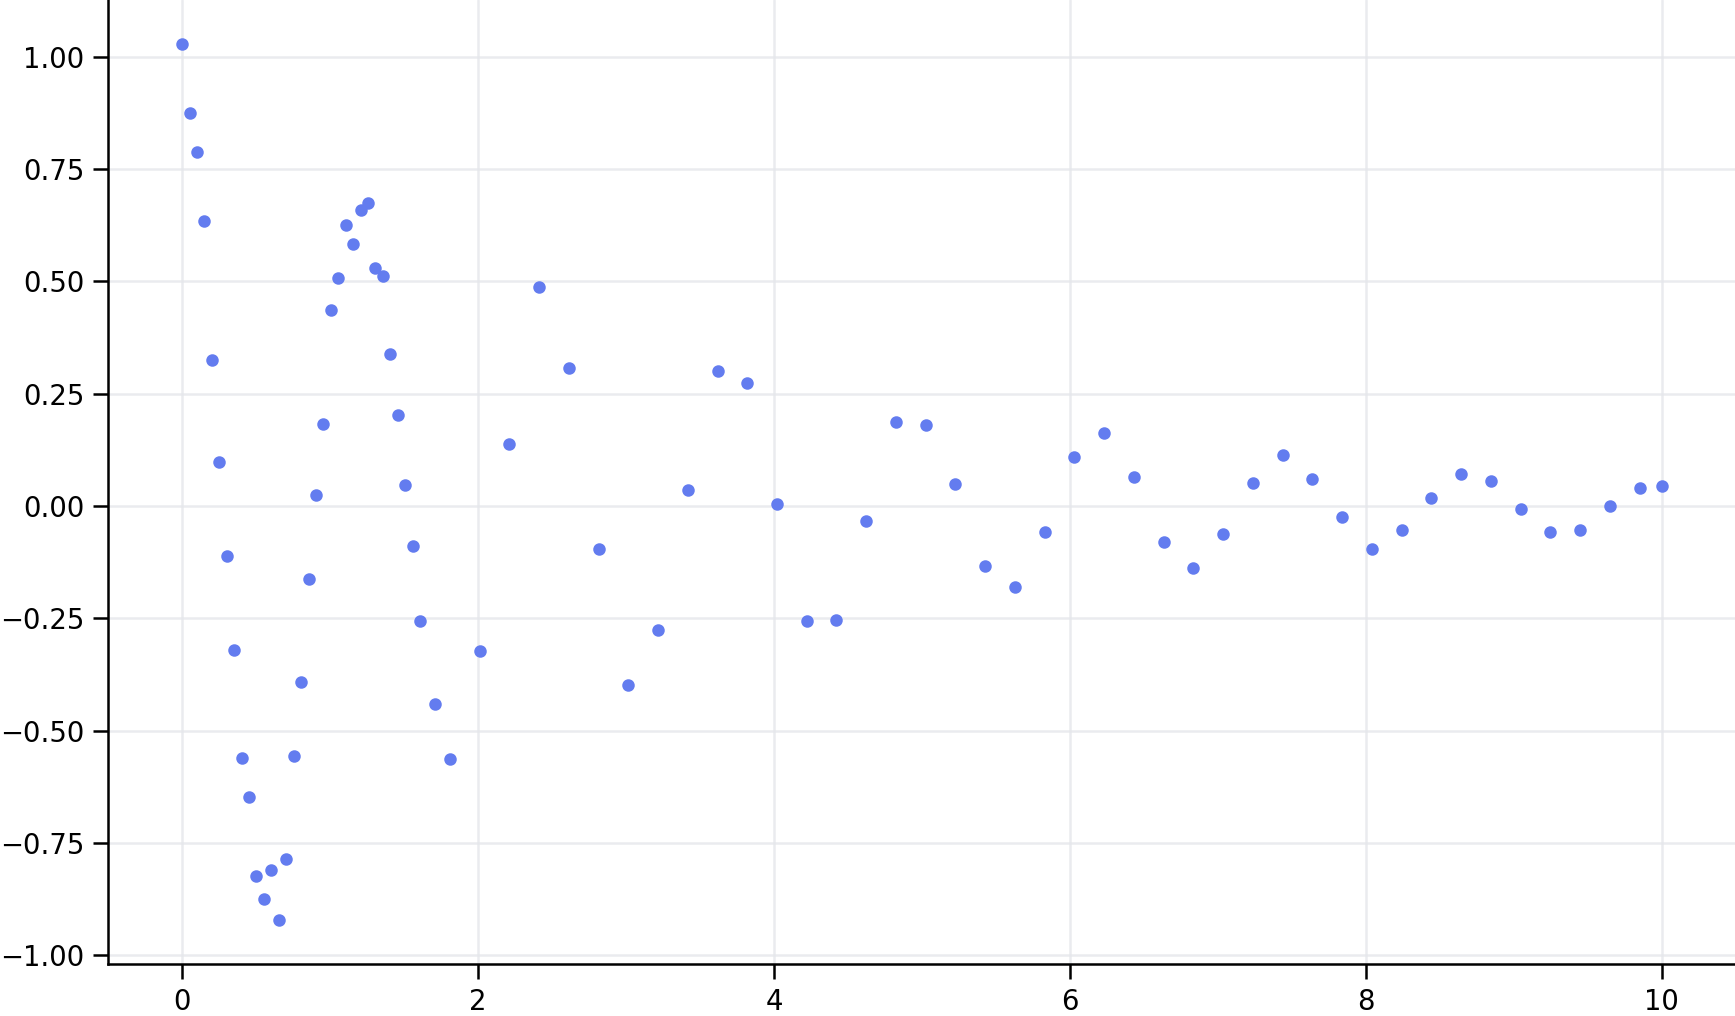
\includegraphics[width=.78\textwidth]{fig_plot_bad2.png}
\caption{Dati rappresentati mediante marker circolari.}
\end{figure}

\section{Etichetta e legenda: \texttt{plot\_bad3.py}}
\begin{lstlisting}
import numpy as np
import matplotlib.pyplot as plt

dati = np.loadtxt("datios.txt")
x = dati[:, 0]
y = dati[:, 1]
plt.plot(x, y, "^", label="Misure")
plt.legend()
plt.show()
\end{lstlisting}

Il marker \texttt{"\string^"} produce triangoli rivolti verso l'alto. L'argomento \texttt{label="Misure"} associa un nome all'oggetto grafico creato da \texttt{plot}. La chiamata \texttt{plt.legend()} raccoglie gli oggetti che possiedono una label e costruisce la legenda.

È importante distinguere i due passaggi: \texttt{label} definisce il testo associato alla serie, mentre \texttt{legend()} rende visibile la legenda. Se si omette \texttt{legend()}, la label rimane associata all'oggetto ma non viene mostrata.

\begin{figure}[H]
\centering
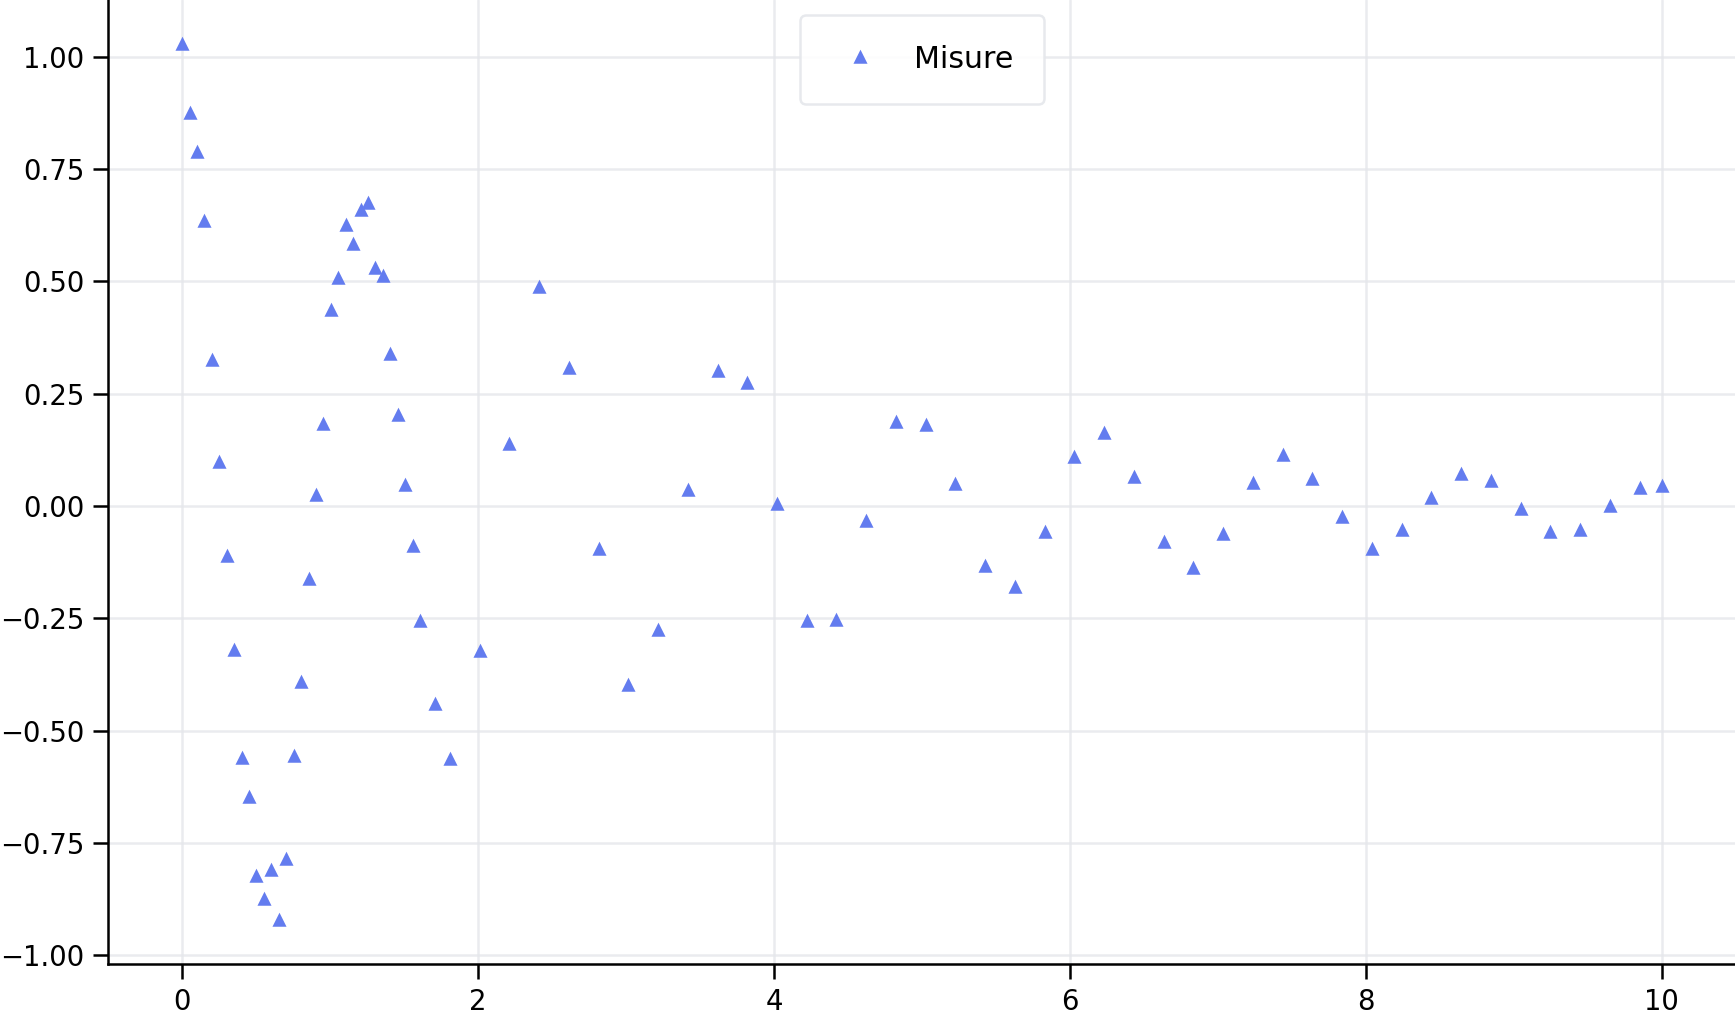
\includegraphics[width=.78\textwidth]{fig_plot_bad3.png}
\caption{Marker triangolari e legenda.}
\end{figure}

\section{Nomi e unità degli assi: \texttt{plot\_bad4.py}}
\begin{lstlisting}
import numpy as np
import matplotlib.pyplot as plt

dati = np.loadtxt("datios.txt")
x = dati[:, 0]
y = dati[:, 1]
plt.plot(x, y, "^", label="Misure")
plt.xlabel("Tempo (s)")
plt.ylabel("Distanza (cm)")
plt.legend()
plt.show()
\end{lstlisting}

Le funzioni \texttt{xlabel} e \texttt{ylabel} descrivono rispettivamente la grandezza riportata sull'asse orizzontale e quella riportata sull'asse verticale. In una figura scientifica si dovrebbero indicare sia il nome della grandezza sia l'unità di misura.

Il testo riportato sugli assi non modifica i dati e non esegue conversioni di unità. Se, per esempio, i dati fossero espressi in metri ma si volessero mostrare in centimetri, sarebbe necessario trasformare numericamente l'array prima del grafico.

\begin{figure}[H]
\centering
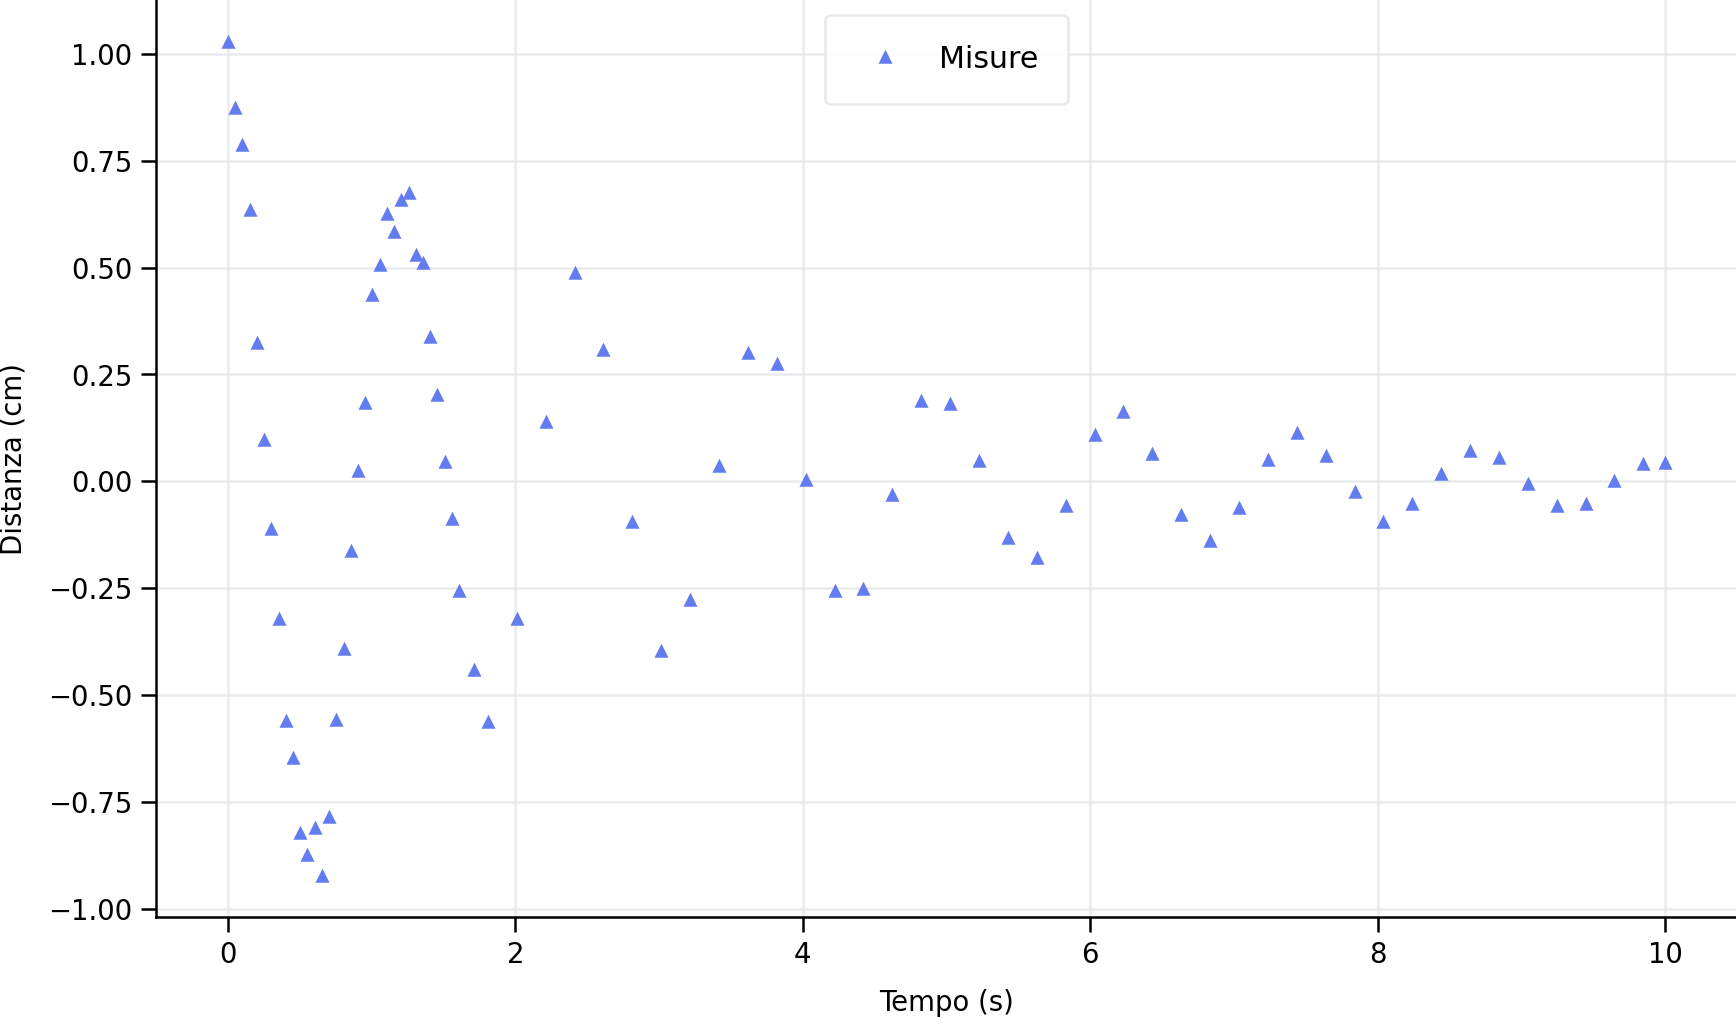
\includegraphics[width=.78\textwidth]{fig_plot_bad4.png}
\caption{Figura completa delle etichette degli assi.}
\end{figure}

\section{Due serie di dati: \texttt{plot\_bad5.py}}
\begin{lstlisting}
import numpy as np
import matplotlib.pyplot as plt

dati = np.loadtxt("Kter.txt")
x = dati[:, 0]
y1 = dati[:, 1]
y2 = dati[:, 2]

plt.plot(x, y1, "^", label="Misure 1")
plt.plot(x, y2, "o", label="Misure 2")
plt.xlabel("Distanza (cm)")
plt.ylabel("Frequenza (Hz)")
plt.legend()
plt.show()
\end{lstlisting}

Questo script legge tre colonne. La prima rappresenta la variabile indipendente comune alle due misure, mentre la seconda e la terza rappresentano due serie diverse. Le due chiamate a \texttt{plot} operano sugli stessi assi e sovrappongono le serie.

Marker e label differenti permettono di distinguere i due insiemi di dati anche quando i colori non sono facilmente riconoscibili. Questa scelta migliora la leggibilità nella stampa in scala di grigi e per utenti con difficoltà nella percezione dei colori.

\begin{figure}[H]
\centering
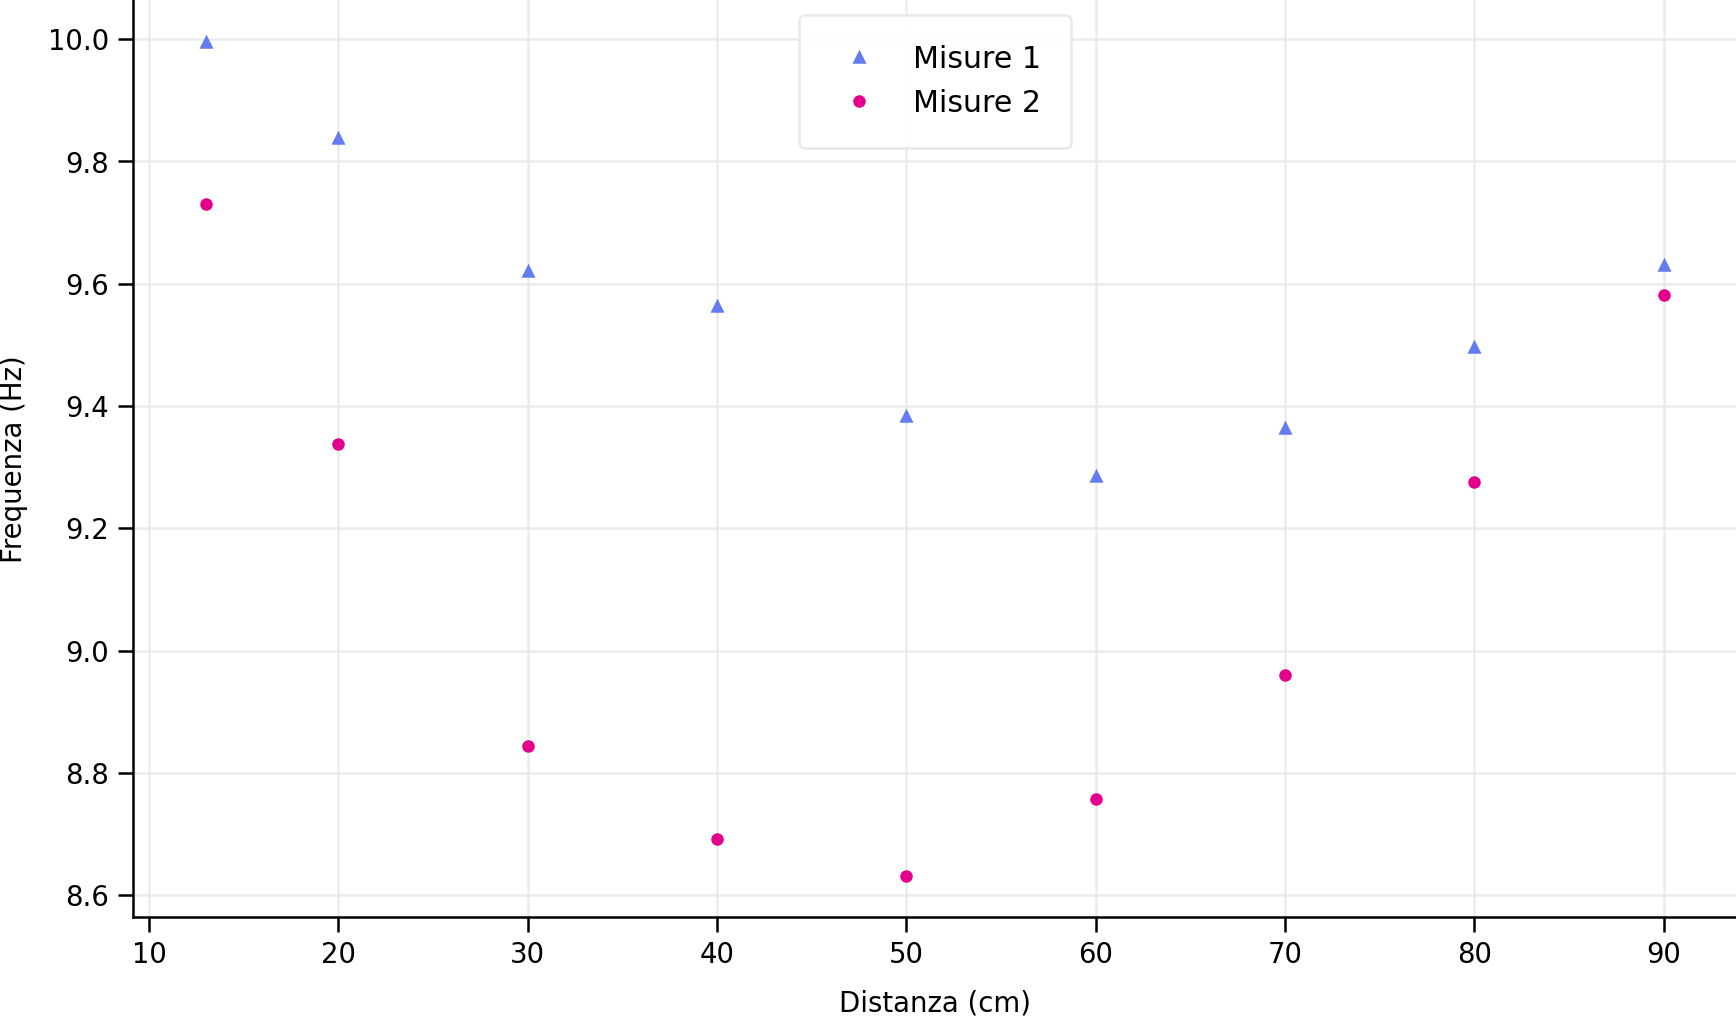
\includegraphics[width=.78\textwidth]{fig_plot_bad5.png}
\caption{Confronto tra due serie di misure.}
\end{figure}

\section{Lettura compatta e salvataggio: \texttt{plot\_bad6.py}}
\begin{lstlisting}
import numpy as np
import matplotlib.pyplot as plt

x, y1, y2 = np.loadtxt("Kter.txt", unpack=True)

plt.plot(x, y1, "^", label="Misure 1")
plt.plot(x, y2, "o", label="Misure 2")
plt.xlabel("Distanza (cm)")
plt.ylabel("Frequenza (Hz)")
plt.legend()

plt.savefig("grafico.pdf")
plt.savefig("grafico.png", dpi=300)
plt.show()
\end{lstlisting}

L'opzione \texttt{unpack=True} traspone concettualmente il risultato della lettura: le colonne vengono restituite come array separati e possono essere assegnate direttamente a \texttt{x}, \texttt{y1} e \texttt{y2}. Questo evita la selezione manuale mediante \texttt{dati[:, i]}.

Le due chiamate a \texttt{savefig} salvano la stessa figura in formati differenti:
\begin{itemize}
  \item il PDF conserva gli elementi grafici in forma vettoriale ed è particolarmente adatto a relazioni e pubblicazioni;
  \item il PNG è un formato raster; il parametro \texttt{dpi=300} richiede una risoluzione elevata, adatta alla stampa.
\end{itemize}

È opportuno salvare la figura prima di \texttt{show()}. Il comportamento di \texttt{show()} dipende dal backend e, in alcuni ambienti, la finestra può essere chiusa o la figura corrente può non essere più disponibile dopo la visualizzazione.

\begin{figure}[H]
\centering
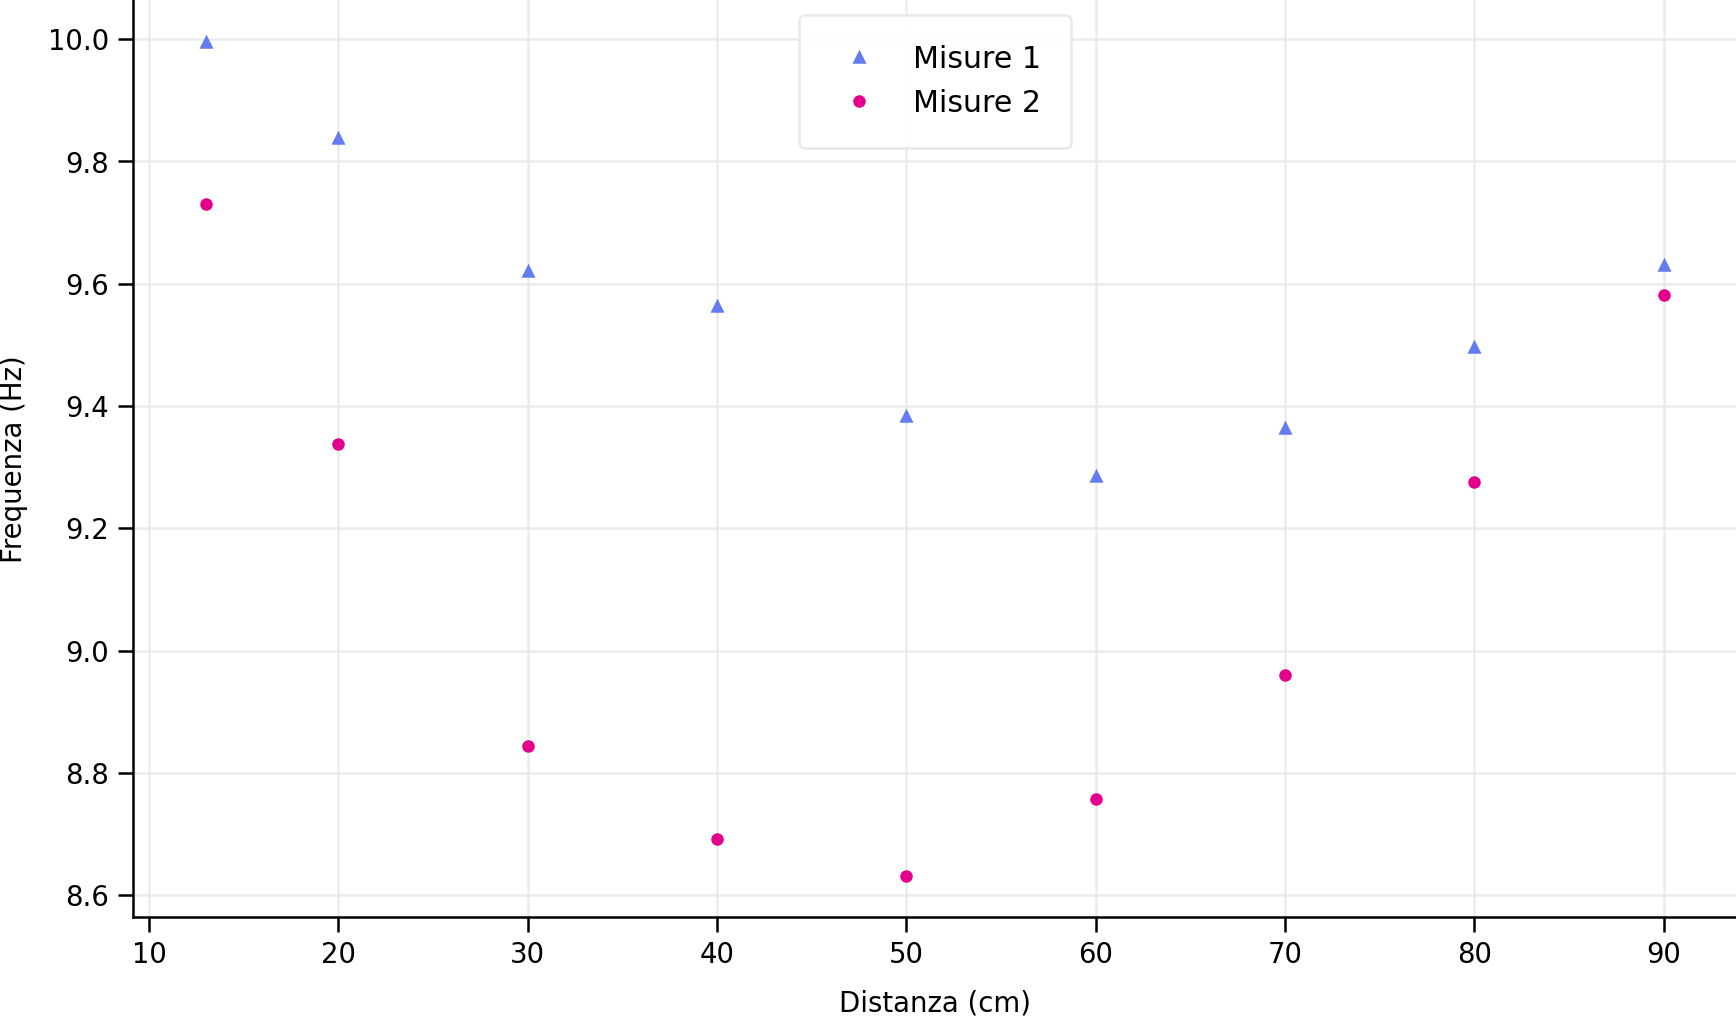
\includegraphics[width=.78\textwidth]{fig_plot_bad6.png}
\caption{Figura a due serie, pronta per essere salvata in PDF e PNG.}
\end{figure}

\section{Versione rifinita: \texttt{plottos2.py}}
\begin{lstlisting}
# Importa NumPy per leggere e manipolare i dati numerici.
import numpy as np

# Importa l'interfaccia grafica pyplot di Matplotlib.
import matplotlib.pyplot as plt

# Importa gli strumenti che controllano la posizione dei tick.
from matplotlib.ticker import MultipleLocator, AutoMinorLocator

# Legge le quattro colonne del file come quattro array separati.
# unpack=True consente l'assegnazione diretta colonna per colonna.
x, y, xerr, yerr = np.loadtxt("datios.txt", unpack=True)

# Crea una figura di 8 x 6 pollici e un sistema di assi.
# fig rappresenta l'intera figura; ax rappresenta gli assi.
fig, ax = plt.subplots(figsize=(8, 6))

# Disegna i punti sperimentali insieme alle barre di errore.
ax.errorbar(
    x,                 # Coordinate orizzontali dei punti.
    y,                 # Coordinate verticali dei punti.
    xerr=xerr,         # Incertezze lungo l'asse x.
    yerr=yerr,         # Incertezze lungo l'asse y.
    fmt="o",           # Marker circolari, senza linea tra i punti.
    color="blue",      # Colore dei marker.
    ecolor="gray",     # Colore delle barre di errore.
    elinewidth=1,      # Spessore delle barre di errore.
    capsize=3,         # Lunghezza dei terminali delle barre.
    markersize=5,      # Dimensione dei marker.
    label="Misura",    # Testo che comparira nella legenda.
)

# Imposta il nome dell'asse x e ne personalizza il carattere.
ax.set_xlabel(
    "Tempo (s)",       # Grandezza e unita di misura.
    fontsize=24,       # Dimensione del carattere.
    fontweight="normal", # Peso normale, quindi non grassetto.
    fontname="Times",  # Famiglia tipografica richiesta.
)

# Imposta il nome dell'asse y con lo stesso stile.
ax.set_ylabel(
    "Distance (cm)",  # Etichetta dell'asse verticale.
    fontsize=24,       # Dimensione del carattere.
    fontweight="normal", # Peso normale.
    fontname="Times", # Famiglia tipografica richiesta.
)

# Personalizza i tick principali di entrambi gli assi.
ax.tick_params(
    axis="both",      # Applica le opzioni agli assi x e y.
    which="major",    # Seleziona soltanto i tick principali.
    labelsize=22,      # Dimensione dei valori numerici.
    width=1.8,         # Spessore dei tick.
    length=7,          # Lunghezza dei tick.
    color="black",    # Colore dei tick.
)

# Personalizza i tick secondari di entrambi gli assi.
ax.tick_params(
    axis="both",      # Applica le opzioni agli assi x e y.
    which="minor",    # Seleziona soltanto i tick secondari.
    width=1.2,         # Spessore dei tick secondari.
    length=4,          # Lunghezza dei tick secondari.
    color="black",    # Colore dei tick secondari.
)

# Riunisce le etichette numeriche dei due assi e le scorre.
for label in ax.get_xticklabels() + ax.get_yticklabels():
    # Imposta il font di ciascuna etichetta numerica.
    label.set_fontname("Times New Roman")

# Colloca un tick principale ogni 1.0 unita sull'asse x.
ax.xaxis.set_major_locator(MultipleLocator(1.0))

# Colloca un tick principale ogni 0.5 unita sull'asse y.
ax.yaxis.set_major_locator(MultipleLocator(0.5))

# Suddivide in cinque parti ogni intervallo principale di x.
ax.xaxis.set_minor_locator(AutoMinorLocator(5))

# Suddivide in cinque parti ogni intervallo principale di y.
ax.yaxis.set_minor_locator(AutoMinorLocator(5))

# Scorre i quattro lati della cornice del grafico.
for spine in ax.spines.values():
    # Imposta lo spessore del lato corrente.
    spine.set_linewidth(1.3)
    # Imposta il colore del lato corrente.
    spine.set_color("black")

# Costruisce la legenda usando le label degli oggetti grafici.
ax.legend(
    loc="best",       # Sceglie automaticamente la posizione.
    # Imposta famiglia e dimensione del font della legenda.
    prop={"family": "Times New Roman", "size": 12},
)

# Ridistribuisce i margini per evitare testi tagliati.
fig.tight_layout()

# Visualizza la figura.
plt.show()
\end{lstlisting}

\subsection{Perché usare \texttt{fig} e \texttt{ax}}
La chiamata
\begin{lstlisting}
fig, ax = plt.subplots(figsize=(8, 6))
\end{lstlisting}
usa l'interfaccia orientata agli oggetti di Matplotlib. \texttt{fig} rappresenta il contenitore complessivo, cioè l'intera figura, mentre \texttt{ax} rappresenta il sistema di assi in cui vengono disegnati dati, etichette e legenda.

Questa impostazione è preferibile nei programmi articolati perché rende esplicito l'oggetto che si sta modificando. Inoltre, consente di gestire facilmente più pannelli nella stessa figura. \texttt{figsize=(8,6)} imposta larghezza e altezza in pollici; la forma $4:3$ è adatta a molte figure scientifiche.

\subsection{Barre di errore con \texttt{ax.errorbar}}
Gli argomenti \texttt{xerr=xerr} e \texttt{yerr=yerr} specificano le incertezze lungo gli assi orizzontale e verticale. Se gli array hanno la stessa lunghezza dei dati, ogni punto possiede la propria incertezza. Un singolo valore scalare, invece, assegnerebbe la stessa incertezza a tutti i punti.

Le principali opzioni grafiche sono:
\begin{description}[style=nextline]
  \item[\texttt{fmt="o"}] usa cerchi come marker e non aggiunge una linea tra i punti;
  \item[\texttt{color="blue"}] imposta il colore dei marker;
  \item[\texttt{ecolor="gray"}] imposta separatamente il colore delle barre di errore;
  \item[\texttt{elinewidth=1}] stabilisce lo spessore delle barre;
  \item[\texttt{capsize=3}] aggiunge piccoli segmenti terminali lunghi tre punti tipografici;
  \item[\texttt{markersize=5}] imposta la dimensione dei marker;
  \item[\texttt{label="Misura"}] assegna alla serie il testo usato dalla legenda.
\end{description}

\subsection{Etichette e caratteri}
I metodi \texttt{ax.set\_xlabel} e \texttt{ax.set\_ylabel} modificano le etichette del singolo oggetto \texttt{ax}. \texttt{fontsize=24} imposta la dimensione, \texttt{fontweight="normal"} il peso e \texttt{fontname} la famiglia tipografica.

Se il font richiesto non è installato, Matplotlib usa un font sostitutivo. Per ottenere un aspetto uniforme è opportuno usare la stessa famiglia per etichette, numeri degli assi e legenda. Nel codice è inoltre consigliabile uniformare la lingua, sostituendo eventualmente \texttt{Distance} con \texttt{Distanza}.

\subsection{Tick principali e secondari}
\texttt{tick\_params} controlla l'aspetto dei tick e delle relative etichette:
\begin{itemize}
  \item \texttt{axis="both"} applica le modifiche a entrambi gli assi;
  \item \texttt{which="major"} o \texttt{which="minor"} seleziona i tick principali o secondari;
  \item \texttt{labelsize} modifica la dimensione dei valori numerici;
  \item \texttt{width} imposta lo spessore dei tick;
  \item \texttt{length} ne imposta la lunghezza;
  \item \texttt{color} ne imposta il colore.
\end{itemize}

Le istruzioni con \texttt{MultipleLocator} stabiliscono il passo delle divisioni principali. Sull'asse $x$ un tick principale compare ogni $1.0$, mentre sull'asse $y$ compare ogni $0.5$. \texttt{AutoMinorLocator(5)} suddivide ciascun intervallo tra due tick principali in cinque parti uguali; di conseguenza, tra due tick principali compaiono quattro tick interni.

\subsection{Cornice, legenda e layout}
Gli elementi di \texttt{ax.spines} rappresentano i quattro lati della cornice. Il ciclo applica lo stesso spessore e lo stesso colore a tutti i lati.

In \texttt{ax.legend}, \texttt{loc="best"} lascia a Matplotlib la scelta della posizione che tende a sovrapporsi meno ai dati. L'argomento \texttt{prop} controlla famiglia e dimensione del carattere della legenda. Infine, \texttt{fig.tight\_layout()} ridistribuisce automaticamente gli spazi per ridurre il rischio che etichette o numeri vengano tagliati ai bordi.

\begin{figure}[H]
\centering
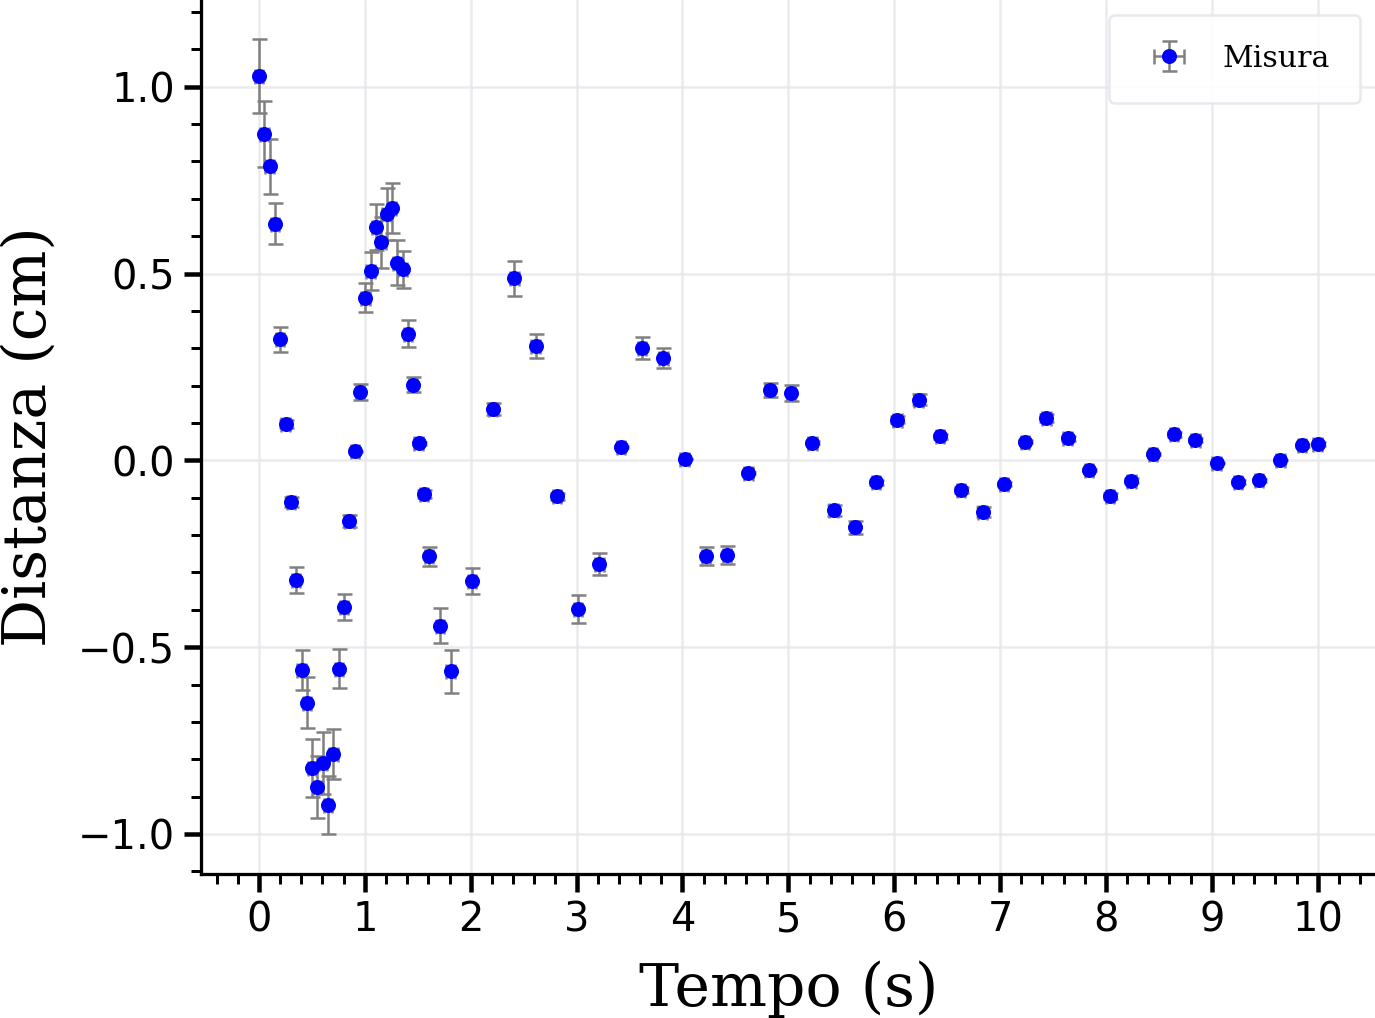
\includegraphics[width=.9\textwidth]{fig_plottos2.png}
\caption{Versione rifinita con barre di errore, tick principali e secondari e stile personalizzato.}
\end{figure}

\chapter{Fit con SciPy e NumPy}

\section{Caso lineare} Gli script assumono che i dati possano essere descritti dal modello lineare 
\[ f(x;m,q)=mx+q, \] 
dove $m$ rappresenta il coefficiente angolare della retta e $q$ la sua intercetta con l'asse delle ordinate. Per ogni punto sperimentale si definisce il residuo
\[ r_i=y_i-f(x_i;m,q) =y_i-(mx_i+q). \] 
Nel caso non pesato, il fit determina i parametri $m$ e $q$ che minimizzano la somma dei quadrati dei residui: 
\[ S(m,q)=\sum_{i=1}^{N} r_i^2 =\sum_{i=1}^{N}\left[y_i-(mx_i+q)\right]^2. \] 
Se sono note le incertezze $\sigma_i$ sulle ordinate, si minimizza invece il chi-quadro
\[ \chi^2(m,q)= \sum_{i=1}^{N} \left[ \frac{y_i-f(x_i;m,q)}{\sigma_i} \right]^2 = \sum_{i=1}^{N} \left[ \frac{y_i-(mx_i+q)}{\sigma_i} \right]^2. \] 
Quando tutte le incertezze sono uguali, minimizzare il chi-quadro equivale, a meno di un fattore costante, a minimizzare la somma dei quadrati dei residui. In questo caso il fit pesato e quello non pesato forniscono quindi gli stessi valori dei parametri $m$ e $q$.

\section{Caso Esempio: Analisi dell'esperimento sul Modulo di Young}

Il programma analizza i dati di un'esperienza di trazione eseguita su un filo metallico e determina il suo \textbf{modulo di Young}. Le grandezze sperimentali direttamente disponibili sono le masse applicate e gli allungamenti prodotti. A partire da esse, il programma calcola:

\begin{itemize}
    \item lo \textbf{sforzo meccanico} $\sigma$;
    \item la \textbf{deformazione} $\varepsilon$;
    \item le rispettive incertezze;
    \item i parametri della relazione lineare tra $\sigma$ ed $\varepsilon$;
    \item il valore del modulo di Young e la sua incertezza.
\end{itemize}

Il risultato viene infine rappresentato graficamente e salvato nel file \texttt{young.pdf}.

\section{Richiami teorici}

\subsection{Sforzo meccanico}

Lo sforzo meccanico, indicato con $\sigma$, è definito come il rapporto tra la forza di trazione $F$ e l'area $S$ della sezione trasversale del filo:

\begin{equation}
    \sigma = \frac{F}{S}.
\end{equation}

Se la forza è prodotta da una massa $m$ soggetta all'accelerazione di gravità $g$, si ha

\begin{equation}
    F=mg
\end{equation}

e quindi

\begin{equation}
    \sigma = \frac{mg}{S}.
\end{equation}

Per un filo di diametro $d$ e sezione circolare,

\begin{equation}
    S=\pi\left(\frac{d}{2}\right)^2.
\end{equation}

Nel Sistema Internazionale lo sforzo si misura in pascal:

\begin{equation}
    1\ \si{\pascal}=1\ \si{\newton\per\square\metre}.
\end{equation}

\subsection{Deformazione}

La deformazione longitudinale convenzionale, o deformazione ingegneristica, è normalmente definita come

\begin{equation}
    \varepsilon=\frac{\Delta L}{L},
\end{equation}

dove $L$ è la lunghezza iniziale e $\Delta L$ è l'allungamento. Essendo il rapporto tra due lunghezze, $\varepsilon$ è adimensionale.

Il codice esaminato utilizza invece

\begin{equation}
    \varepsilon=\frac{\Delta L}{L+\Delta L}.
\end{equation}

Questa scelta deve essere verificata rispetto alla definizione adottata nell'esperienza. Nella descrizione che segue viene mantenuta esattamente la formula presente nel programma.

\subsection{Legge di Hooke e modulo di Young}

Nel regime elastico lineare, sforzo e deformazione sono legati dalla relazione

\begin{equation}
    \sigma=Y\varepsilon,
\end{equation}

dove $Y$ è il modulo di Young. Il programma adotta un modello leggermente più generale:

\begin{equation}
    \sigma=Y\varepsilon+I,
\end{equation}

in cui $I$ è l'intercetta. In un esperimento ideale ci si aspetterebbe $I=0$; lasciarla libera permette però di descrivere un eventuale offset sperimentale.

\section{Struttura attesa del file di dati}

Il programma legge il file \texttt{yang.dat}. Dal modo in cui le colonne vengono utilizzate si ricava la seguente struttura:

\begin{center}
\begin{tabular}{cl}
\toprule
Colonna & Contenuto utilizzato dal programma \\
\midrule
0 & massa applicata, dichiarata in grammi \\
1 & allungamento $\Delta L$, dichiarato in millimetri \\
2 & incertezza sulla massa \\
3 & incertezza sull'allungamento \\
\bottomrule
\end{tabular}
\end{center}

Il file deve quindi contenere almeno quattro colonne numeriche, separate da spazi o tabulazioni. Tutte le righe devono avere una struttura compatibile con la lettura eseguita da \texttt{numpy.loadtxt()}.

\section{Codice completo}

Il listato seguente riproduce integralmente il programma analizzato.

\begin{lstlisting}[caption={Codice completo del programma \texttt{young.py}},label={lst:young}]
import numpy as np
import matplotlib.pyplot as plt
from scipy.optimize import curve_fit

# Carica i dati: prima colonna = masse (g), seconda = allungamenti (mm)
dati = np.loadtxt("yang.dat")

# Calcolo dello sforzo sigma = F/S = m * g / (pi * (d/2)^2)
masse = dati[:, 0] / 1000  # conversione in kg
g = 9.81  # accelerazione gravitazionale
d = 0.29 / 1000  # diametro in metri
area = np.pi * (d / 2)**2
sigma = masse * g / area  # in N/m^2

# Calcolo della deformazione epsilon = DeltaL / L
delta_l = dati[:, 1]  # in mm
L = 2000  # lunghezza iniziale in mm
epsilon = delta_l / (L + delta_l)  # adimensionale

# Errori su sigma e epsilon
err_masse = dati[:, 2]
err_deformazioni = dati[:, 3]
err_sigma = err_masse * g / area
err_epsilon = (L / (L + epsilon)**2) * err_deformazioni

# Fit lineare: sigma = Y * epsilon
def retta(x, Y, I):
    return Y * x + I

popt, pcov = curve_fit(
    retta,
    epsilon,
    sigma,
    sigma=err_sigma,
    maxfev=10000000,
    p0=[1E11, 1E8]
)

modulo_di_young = popt[0]
errore_modulo = np.sqrt(np.diag(pcov))[0]

# Stampa del risultato
print(
    f"Il modulo di Young vale: {modulo_di_young:.5e} "
    f"+/- {errore_modulo:.3e} (N/m^2)"
)

# Grafico
plt.figure(figsize=(8, 6))
plt.plot(epsilon, sigma, 'bo', label='Misure')
plt.plot(epsilon, retta(epsilon, *popt), 'r-', label='Fit lineare')
plt.xlabel("Deformazione epsilon = DeltaL / L")
plt.ylabel("Sforzo sigma (N/m^2)")
plt.title("Calcolo del Modulo di Young")
plt.legend()
plt.grid(True)

# Annotazione del risultato
plt.text(
    0.00005,
    max(sigma) * 0.9,
    f"Y = {modulo_di_young:.4e} +/- {errore_modulo:.3e} N/m^2",
    fontsize=10
)

plt.savefig("young.pdf")
plt.show()
\end{lstlisting}

Nel listato sono stati sostituiti, nelle sole stringhe visualizzate, alcuni simboli Unicode con equivalenti ASCII per rendere la compilazione LaTeX più robusta. La logica numerica del programma rimane invariata.
Il risultato finale dello script è riportato in figura \ref{fig:young}.

\begin{figure}
    \centering
    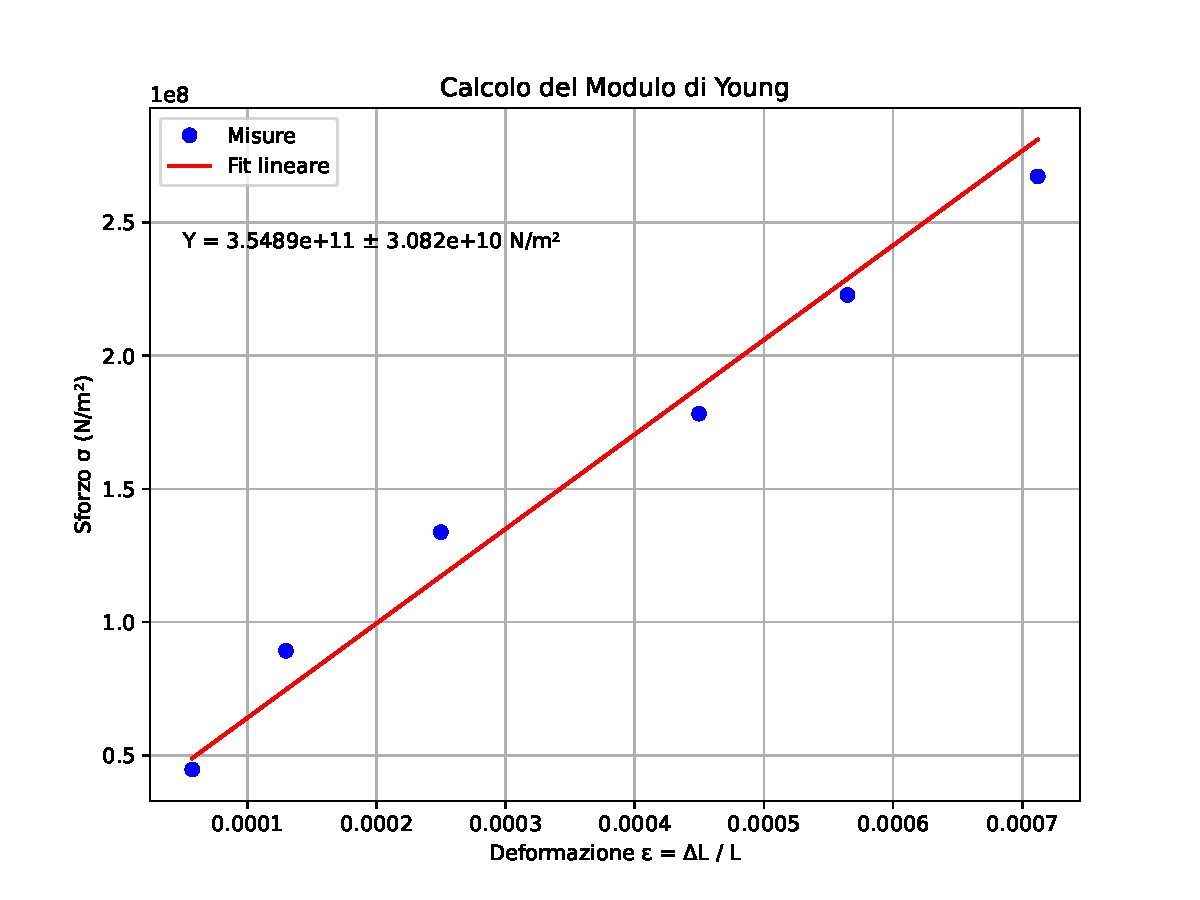
\includegraphics[width=0.8\linewidth]{young.pdf}
    \caption{Risultato dello script \ref{lst:young}.}
    \label{fig:young}
\end{figure}

\section{Analisi dettagliata del codice}

\subsection{Importazione delle librerie}

\begin{lstlisting}
import numpy as np
import matplotlib.pyplot as plt
from scipy.optimize import curve_fit
\end{lstlisting}

\begin{itemize}
    \item \texttt{NumPy} viene utilizzato per leggere i dati, eseguire operazioni vettoriali e manipolare la matrice di covarianza;
    \item \texttt{Matplotlib} serve a costruire e salvare il grafico;
    \item \texttt{curve\_fit}, appartenente a \texttt{scipy.optimize}, esegue il fit non lineare ai minimi quadrati. In questo caso il modello è lineare nei parametri, ma viene comunque trattato attraverso l'interfaccia generale di \texttt{curve\_fit}.
\end{itemize}

Gli alias \texttt{np} e \texttt{plt} sono abbreviazioni convenzionali che rendono il codice più compatto.

\subsection{Lettura dei dati}

\begin{lstlisting}
dati = np.loadtxt("yang.dat")
\end{lstlisting}

La funzione \texttt{np.loadtxt()} legge il file e costruisce un array bidimensionale. Ogni riga del file diventa una riga dell'array; ogni colonna del file diventa una colonna dell'array.

L'espressione

\begin{lstlisting}
dati[:, 0]
\end{lstlisting}

usa lo slicing bidimensionale:

\begin{itemize}
    \item i due punti, \texttt{:}, selezionano tutte le righe;
    \item \texttt{0} seleziona la prima colonna.
\end{itemize}

Analogamente, \texttt{dati[:, 1]}, \texttt{dati[:, 2]} e \texttt{dati[:, 3]} selezionano rispettivamente la seconda, la terza e la quarta colonna.

\subsection{Conversione della massa}

\begin{lstlisting}
masse = dati[:, 0] / 1000
\end{lstlisting}

La prima colonna contiene masse espresse in grammi. La divisione per 1000 le converte in chilogrammi:

\begin{equation}
    m_{\si{kg}}=\frac{m_{\si{g}}}{1000}.
\end{equation}

L'operazione viene applicata contemporaneamente a tutti gli elementi della colonna, senza bisogno di un ciclo esplicito.

\subsection{Costanti e area della sezione}

\begin{lstlisting}
g = 9.81
d = 0.29 / 1000
area = np.pi * (d / 2)**2
\end{lstlisting}

Il valore di $g$ è fissato a $9{,}81\ \si{\metre\per\second\squared}$. Il diametro, inizialmente espresso in millimetri, viene convertito in metri:

\begin{equation}
    d=\frac{0{,}29}{1000}\ \si{\metre}.
\end{equation}

In Python l'operatore \texttt{**} rappresenta l'elevamento a potenza. Pertanto \texttt{(d/2)**2} corrisponde a $(d/2)^2$.

\subsection{Calcolo dello sforzo}

\begin{lstlisting}
sigma = masse * g / area
\end{lstlisting}

Questa istruzione traduce direttamente la formula

\begin{equation}
    \sigma=\frac{mg}{\pi(d/2)^2}.
\end{equation}

Poiché le masse sono contenute in un array, NumPy calcola automaticamente un valore di $\sigma$ per ciascuna misura.

\subsection{Calcolo della deformazione}

\begin{lstlisting}
delta_l = dati[:, 1]
L = 2000
epsilon = delta_l / (L + delta_l)
\end{lstlisting}

La seconda colonna viene assegnata all'array \texttt{delta\_l}. La lunghezza iniziale è fissata a $L=2000\ \si{\milli\metre}$. Poiché sia $L$ sia $\Delta L$ sono espressi in millimetri, il rapporto è adimensionale.

La riga di codice implementa

\begin{equation}
    \varepsilon=\frac{\Delta L}{L+\Delta L}.
\end{equation}

Il commento presente nel programma riporta invece $\varepsilon=\Delta L/L$. È quindi opportuno rendere coerenti formula, commento e definizione fisica adottata.

\subsection{Lettura delle incertezze}

\begin{lstlisting}
err_masse = dati[:, 2]
err_deformazioni = dati[:, 3]
\end{lstlisting}

La terza e la quarta colonna vengono interpretate rispettivamente come incertezze sulle masse e sugli allungamenti.

\subsection{Propagazione dell'incertezza sullo sforzo}

\begin{lstlisting}
err_sigma = err_masse * g / area
\end{lstlisting}

Assumendo trascurabili le incertezze su $g$ e sull'area, dalla relazione

\begin{equation}
    \sigma(m)=\frac{mg}{S}
\end{equation}

si ricava

\begin{equation}
    \Delta\sigma=
    \left|\frac{\partial\sigma}{\partial m}\right|\Delta m
    =\frac{g}{S}\Delta m.
\end{equation}

È essenziale che \texttt{err\_masse} sia espresso in chilogrammi. Se la terza colonna di \texttt{yang.dat} è in grammi, deve essere convertita dividendo anch'essa per 1000 prima di calcolare \texttt{err\_sigma}.

\subsection{Propagazione dell'incertezza sulla deformazione}

Nel programma compare:

\begin{lstlisting}
err_epsilon = (L / (L + epsilon)**2) * err_deformazioni
\end{lstlisting}

Se la definizione utilizzata è

\begin{equation}
    \varepsilon(\Delta L)=\frac{\Delta L}{L+\Delta L},
\end{equation}

la derivata corretta rispetto a $\Delta L$ è

\begin{equation}
    \frac{\partial\varepsilon}{\partial(\Delta L)}
    =\frac{L}{(L+\Delta L)^2}.
\end{equation}

Di conseguenza, trascurando l'incertezza su $L$,

\begin{equation}
    \Delta\varepsilon=
    \frac{L}{(L+\Delta L)^2}\,\Delta(\Delta L).
\end{equation}

Nel codice, al denominatore compare \texttt{L + epsilon}, mentre dimensionalmente dovrebbe comparire \texttt{L + delta\_l}. Inoltre l'array \texttt{err\_epsilon} viene calcolato ma non viene successivamente passato al fit né rappresentato nel grafico.

\subsection{Definizione del modello}

\begin{lstlisting}
def retta(x, Y, I):
    return Y * x + I
\end{lstlisting}

La funzione riceve tre argomenti:

\begin{itemize}
    \item \texttt{x}: variabile indipendente, che nel fit sarà $\varepsilon$;
    \item \texttt{Y}: coefficiente angolare, identificato con il modulo di Young;
    \item \texttt{I}: intercetta della retta.
\end{itemize}

La funzione restituisce l'array dei valori

\begin{equation}
    y=Yx+I.
\end{equation}

\subsection{Esecuzione del fit}

\begin{lstlisting}
popt, pcov = curve_fit(
    retta,
    epsilon,
    sigma,
    sigma=err_sigma,
    maxfev=10000000,
    p0=[1E11, 1E8]
)
\end{lstlisting}

Gli argomenti hanno il seguente significato:

\begin{itemize}
    \item \texttt{retta}: funzione modello;
    \item \texttt{epsilon}: valori della variabile indipendente;
    \item \texttt{sigma}: valori sperimentali della variabile dipendente;
    \item \texttt{sigma=err\_sigma}: incertezze associate ai valori di $\sigma$, utilizzate come pesi del fit;
    \item \texttt{p0=[1E11, 1E8]}: valori iniziali proposti per $Y$ e $I$;
    \item \texttt{maxfev=10000000}: numero massimo di valutazioni della funzione consentite durante l'ottimizzazione.
\end{itemize}

La notazione \texttt{1E11} indica $1\times 10^{11}$, mentre \texttt{1E8} indica $1\times 10^8$.

Il fit minimizza una quantità del tipo

\begin{equation}
    \chi^2=\sum_i
    \left[
    \frac{\sigma_i-f(\varepsilon_i;Y,I)}{\Delta\sigma_i}
    \right]^2.
\end{equation}

Poiché il codice non imposta \texttt{absolute\_sigma=True}, la matrice di covarianza restituita da \texttt{curve\_fit} viene riscalata secondo il comportamento predefinito della funzione. Se \texttt{err\_sigma} rappresenta incertezze assolute note, può essere opportuno valutare l'uso di \texttt{absolute\_sigma=True}.

\subsection{Parametri ottimali e matrice di covarianza}

\texttt{curve\_fit} restituisce:

\begin{itemize}
    \item \texttt{popt}, array dei parametri ottimali;
    \item \texttt{pcov}, matrice di covarianza dei parametri.
\end{itemize}

Nel caso considerato,

\begin{equation}
    \texttt{popt[0]}=Y,
    \qquad
    \texttt{popt[1]}=I.
\end{equation}

La matrice di covarianza ha forma

\begin{equation}
    \mathbf{C}=
    \begin{pmatrix}
    \operatorname{Var}(Y) & \operatorname{Cov}(Y,I)\\
    \operatorname{Cov}(I,Y) & \operatorname{Var}(I)
    \end{pmatrix}.
\end{equation}

Gli elementi diagonali sono le varianze dei parametri. Le rispettive incertezze standard si ottengono calcolandone la radice quadrata.

\begin{lstlisting}
modulo_di_young = popt[0]
errore_modulo = np.sqrt(np.diag(pcov))[0]
\end{lstlisting}

La funzione \texttt{np.diag(pcov)} estrae gli elementi diagonali; \texttt{np.sqrt()} ne calcola la radice quadrata; l'indice \texttt{[0]} seleziona l'incertezza del primo parametro, cioè $Y$.

\subsection{Stampa del risultato}

\begin{lstlisting}
print(
    f"Il modulo di Young vale: {modulo_di_young:.5e} "
    f"+/- {errore_modulo:.3e} (N/m^2)"
)
\end{lstlisting}

La stringa preceduta da \texttt{f} è una \emph{f-string}. Le espressioni racchiuse tra parentesi graffe vengono valutate e inserite nel testo.

Il formato \texttt{.5e} stampa il valore in notazione scientifica con cinque cifre dopo il punto decimale; \texttt{.3e} ne utilizza tre.

\section{Costruzione del grafico}

\subsection{Creazione della figura}

\begin{lstlisting}
plt.figure(figsize=(8, 6))
\end{lstlisting}

Viene creata una figura di larghezza 8 pollici e altezza 6 pollici.

\subsection{Rappresentazione delle misure}

\begin{lstlisting}
plt.plot(epsilon, sigma, 'bo', label='Misure')
\end{lstlisting}

La stringa di formato \texttt{'bo'} significa:

\begin{itemize}
    \item \texttt{b}: colore blu;
    \item \texttt{o}: marcatore circolare.
\end{itemize}

Ogni coppia $(\varepsilon_i,\sigma_i)$ viene rappresentata da un punto blu.

\subsection{Rappresentazione della retta di fit}

\begin{lstlisting}
plt.plot(epsilon, retta(epsilon, *popt), 'r-', label='Fit lineare')
\end{lstlisting}

L'operatore \texttt{*} davanti a \texttt{popt} esegue l'unpacking dell'array. Se

\begin{equation}
    \texttt{popt}=[Y,I],
\end{equation}

allora

\begin{lstlisting}
retta(epsilon, *popt)
\end{lstlisting}

equivale a

\begin{lstlisting}
retta(epsilon, popt[0], popt[1])
\end{lstlisting}

La stringa \texttt{'r-'} richiede una linea continua rossa.

\subsection{Etichette, titolo, legenda e griglia}

\begin{lstlisting}
plt.xlabel("Deformazione epsilon = DeltaL / L")
plt.ylabel("Sforzo sigma (N/m^2)")
plt.title("Calcolo del Modulo di Young")
plt.legend()
plt.grid(True)
\end{lstlisting}

\texttt{xlabel()} e \texttt{ylabel()} definiscono le etichette degli assi; \texttt{title()} imposta il titolo; \texttt{legend()} mostra la legenda costruita usando gli argomenti \texttt{label}; \texttt{grid(True)} attiva la griglia.

\subsection{Annotazione nella figura}

\begin{lstlisting}
plt.text(
    0.00005,
    max(sigma) * 0.9,
    f"Y = {modulo_di_young:.4e} +/- {errore_modulo:.3e} N/m^2",
    fontsize=10
)
\end{lstlisting}

La funzione \texttt{plt.text()} inserisce un testo alle coordinate specificate. La coordinata orizzontale è fissata a $5\times10^{-5}$; quella verticale è posta al 90\% del massimo valore di $\sigma$.

Questa scelta funziona soltanto se tali coordinate ricadono nell'intervallo visualizzato. Una soluzione più generale può usare coordinate relative agli assi, ma il listato mantiene la scelta originale.

\subsection{Salvataggio e visualizzazione}

\begin{lstlisting}
plt.savefig("young.pdf")
plt.show()
\end{lstlisting}

\texttt{savefig()} salva la figura in formato PDF. \texttt{show()} apre la finestra grafica e visualizza il risultato.

\section{Osservazioni sul trattamento degli errori}

\subsection{Errori verticali non rappresentati}

Il fit utilizza \texttt{err\_sigma}, ma il grafico mostra i punti mediante \texttt{plt.plot()}, senza barre d'errore. Per visualizzare le incertezze verticali sarebbe possibile utilizzare \texttt{plt.errorbar()}.

\subsection{Errori sulla variabile indipendente}

L'array \texttt{err\_epsilon} non viene utilizzato nel fit. \texttt{curve\_fit} tratta direttamente le incertezze sulla variabile dipendente, ma non quelle sulla variabile indipendente. Se le incertezze su $\varepsilon$ non sono trascurabili, può essere necessario adottare un metodo che tenga conto degli errori su entrambi gli assi, come l'\emph{Orthogonal Distance Regression}.

\subsection{Incertezza sul diametro}

L'area dipende dal quadrato del diametro. Un'eventuale incertezza su $d$ produce quindi un contributo all'incertezza sullo sforzo. Il codice considera il diametro esatto e propaga soltanto l'incertezza sulla massa.

\subsection{Intercetta e significato fisico}

Il modello include un'intercetta libera. Se l'esperienza richiede teoricamente il passaggio per l'origine, si possono confrontare due strategie:

\begin{enumerate}
    \item fit con intercetta libera, utile per individuare un offset;
    \item fit vincolato all'origine, utile se l'assenza di intercetta è una condizione fisica giustificata.
\end{enumerate}

La scelta non dovrebbe essere effettuata soltanto sulla base dell'aspetto grafico, ma deve essere coerente con il modello sperimentale.

\section{Controlli consigliati}

Prima di interpretare il risultato finale è opportuno verificare:

\begin{enumerate}
    \item le unità della terza e della quarta colonna di \texttt{yang.dat};
    \item la definizione di deformazione adottata nell'esperienza;
    \item la formula di propagazione usata per \texttt{err\_epsilon};
    \item l'eventuale incertezza sul diametro del filo;
    \item se le incertezze fornite a \texttt{curve\_fit} siano assolute;
    \item se l'intercetta debba essere libera oppure vincolata a zero;
    \item se i dati appartengano interamente al regime elastico lineare.
\end{enumerate}

\section{Commenti finali sul caso modulo di Young}

Il programma mostra una procedura completa di analisi sperimentale: legge i dati da file, converte le unità di misura, calcola le grandezze fisiche, propaga alcune incertezze, esegue un fit pesato e produce una rappresentazione grafica.

Il coefficiente angolare della retta di fit viene interpretato come modulo di Young. La matrice di covarianza consente di ricavare l'incertezza associata al parametro. Restano tuttavia da verificare la definizione della deformazione, la propagazione della sua incertezza e la coerenza delle unità usate per l'errore sulla massa.








% Capitolo da inserire in un documento che carichi almeno:
% \usepackage{amsmath}
% \usepackage{xcolor}
% \usepackage{listings}
% \usepackage{booktabs}
%
% Si assume inoltre che sia definito uno stile listings per Python.



\section{Caso parabolico}
Gli script assumono che i dati possano essere descritti dal modello
\[
 f(x;a,b,c)=ax^2+bx+c.
\]
Per ogni punto sperimentale si definisce il residuo
\[
 r_i=y_i-f(x_i;a,b,c).
\]
Nel caso non pesato, il fit determina i parametri che minimizzano
\[
 S(a,b,c)=\sum_{i=1}^{N}r_i^2.
\]
Se sono note le incertezze $\sigma_i$ sulle ordinate, si minimizza invece il chi-quadro
\[
 \chi^2(a,b,c)=\sum_{i=1}^{N}
 \left[\frac{y_i-f(x_i;a,b,c)}{\sigma_i}\right]^2.
\]
Quando tutte le incertezze sono uguali, minimizzare il chi-quadro equivale, a meno di un fattore costante, a minimizzare la somma dei quadrati dei residui.

\section{Fit con \texttt{scipy.optimize.curve\_fit}}
\begin{lstlisting}
# Importa NumPy per lettura, array e funzioni numeriche.
import numpy as np

# Importa Matplotlib per costruire il grafico.
import matplotlib.pyplot as plt

# Importa la funzione di fit generale di SciPy.
from scipy.optimize import curve_fit

# Definisce il modello: una parabola nei parametri a, b e c.
def parabola(x, a, b, c):
    # Restituisce il valore del modello per ogni elemento di x.
    return a*x**2 + b*x + c

# Legge le tre colonne come array x, y1 e y2.
x, y1, y2 = np.loadtxt("Kter.txt", unpack=True)

# Adatta la parabola alla prima serie di misure.
# popt1 contiene [a, b, c]; pcov1 e la loro covarianza.
popt1, pcov1 = curve_fit(parabola, x, y1)

# Ripete il fit per la seconda serie di misure.
popt2, pcov2 = curve_fit(parabola, x, y2)

# Estrae le varianze dalla diagonale e calcola gli errori.
perr1 = np.sqrt(np.diag(pcov1))

# Calcola le incertezze standard dei parametri del secondo fit.
perr2 = np.sqrt(np.diag(pcov2))

# Crea 500 valori di x per disegnare curve regolari.
xfit = np.linspace(np.min(x), np.max(x), 500)

# Disegna la prima serie con marker triangolari.
plt.plot(x, y1, "^", label="Misure 1")

# Disegna la seconda serie con marker circolari.
plt.plot(x, y2, "o", label="Misure 2")

# Disegna in rosso la parabola del primo fit.
# *popt1 spacchetta l'array nei tre parametri a, b e c.
plt.plot(
    xfit,
    parabola(xfit, *popt1),
    "r-",
    lw=2,
    label="Fit 1",
)

# Disegna in blu la parabola del secondo fit.
plt.plot(
    xfit,
    parabola(xfit, *popt2),
    "b-",
    lw=2,
    label="Fit 2",
)

# Imposta il nome e l'unita dell'asse orizzontale.
plt.xlabel("Distanza (cm)")

# Imposta il nome e l'unita dell'asse verticale.
plt.ylabel("Frequenza (Hz)")

# Costruisce la legenda.
plt.legend()

# Salva una versione vettoriale della figura.
plt.savefig("grafico.pdf")

# Salva una versione raster a 300 punti per pollice.
plt.savefig("grafico.png", dpi=300)

# Visualizza la figura.
plt.show()
\end{lstlisting}

\subsection{Definizione del modello}
La funzione \texttt{parabola} riceve come primo argomento la variabile indipendente e, successivamente, i parametri da determinare. Questa struttura è richiesta da \texttt{curve\_fit}. Il vantaggio è che il modello non deve essere necessariamente un polinomio: può essere una funzione esponenziale, gaussiana, trigonometrica oppure una combinazione più complessa.

\subsection{Minimizzazione e chi-quadro}
\texttt{curve\_fit} esegue un fit ai minimi quadrati non lineari. Se \texttt{sigma} non viene specificato, il programma assume pesi uguali, equivalenti a un array di incertezze tutte unitarie, e minimizza la somma dei quadrati dei residui. Se si fornisce un array monodimensionale \texttt{sigma}, la funzione minimizzata è
\[
 \chi^2=\sum_i\left(\frac{r_i}{\sigma_i}\right)^2.
\]
Pertanto, è corretto descrivere \texttt{curve\_fit} come una procedura di minimizzazione del chi-quadro quando le incertezze sono esplicitamente fornite; senza \texttt{sigma}, si tratta del caso non pesato dello stesso schema.

Per un fit pesato si scrive:
\begin{lstlisting}
popt, pcov = curve_fit(
    parabola,
    x,
    y,
    sigma=yerr,
    absolute_sigma=True,
)
\end{lstlisting}
Con \texttt{absolute\_sigma=True}, le incertezze fornite sono interpretate in senso assoluto e la matrice di covarianza dei parametri mantiene questa normalizzazione. Con il valore predefinito \texttt{False}, conta inizialmente la scala relativa delle incertezze e la covarianza viene riscalata in relazione al chi-quadro ridotto ottenuto.

Per problemi senza vincoli, \texttt{curve\_fit} usa normalmente l'algoritmo di Levenberg--Marquardt. In presenza di limiti sui parametri passa a metodi compatibili con i vincoli, come il Trust Region Reflective. Nel caso della parabola il modello è lineare nei parametri $a$, $b$ e $c$, anche se \texttt{curve\_fit} viene utilizzato attraverso la sua interfaccia generale per fit non lineari.

\subsection{Parametri restituiti e operatore \texttt{*}}
\texttt{popt1} contiene i parametri ottimali nell'ordine con cui compaiono nella funzione:
\[
 \texttt{popt1}=[a,b,c].
\]
L'espressione \texttt{parabola(xfit, *popt1)} usa l'operatore di spacchettamento \texttt{*}: i tre elementi dell'array sono passati alla funzione come tre argomenti distinti.

\subsection{Costruzione della curva continua}
\texttt{np.linspace} genera 500 punti equidistanti tra il minimo e il massimo valore di $x$. Il fit viene valutato su questa griglia più fitta, non soltanto nei punti sperimentali. In questo modo la curva appare regolare. I dati restano rappresentati con marker, mentre il modello è mostrato con una linea continua di spessore \texttt{lw=2}.

\begin{figure}[H]
\centering
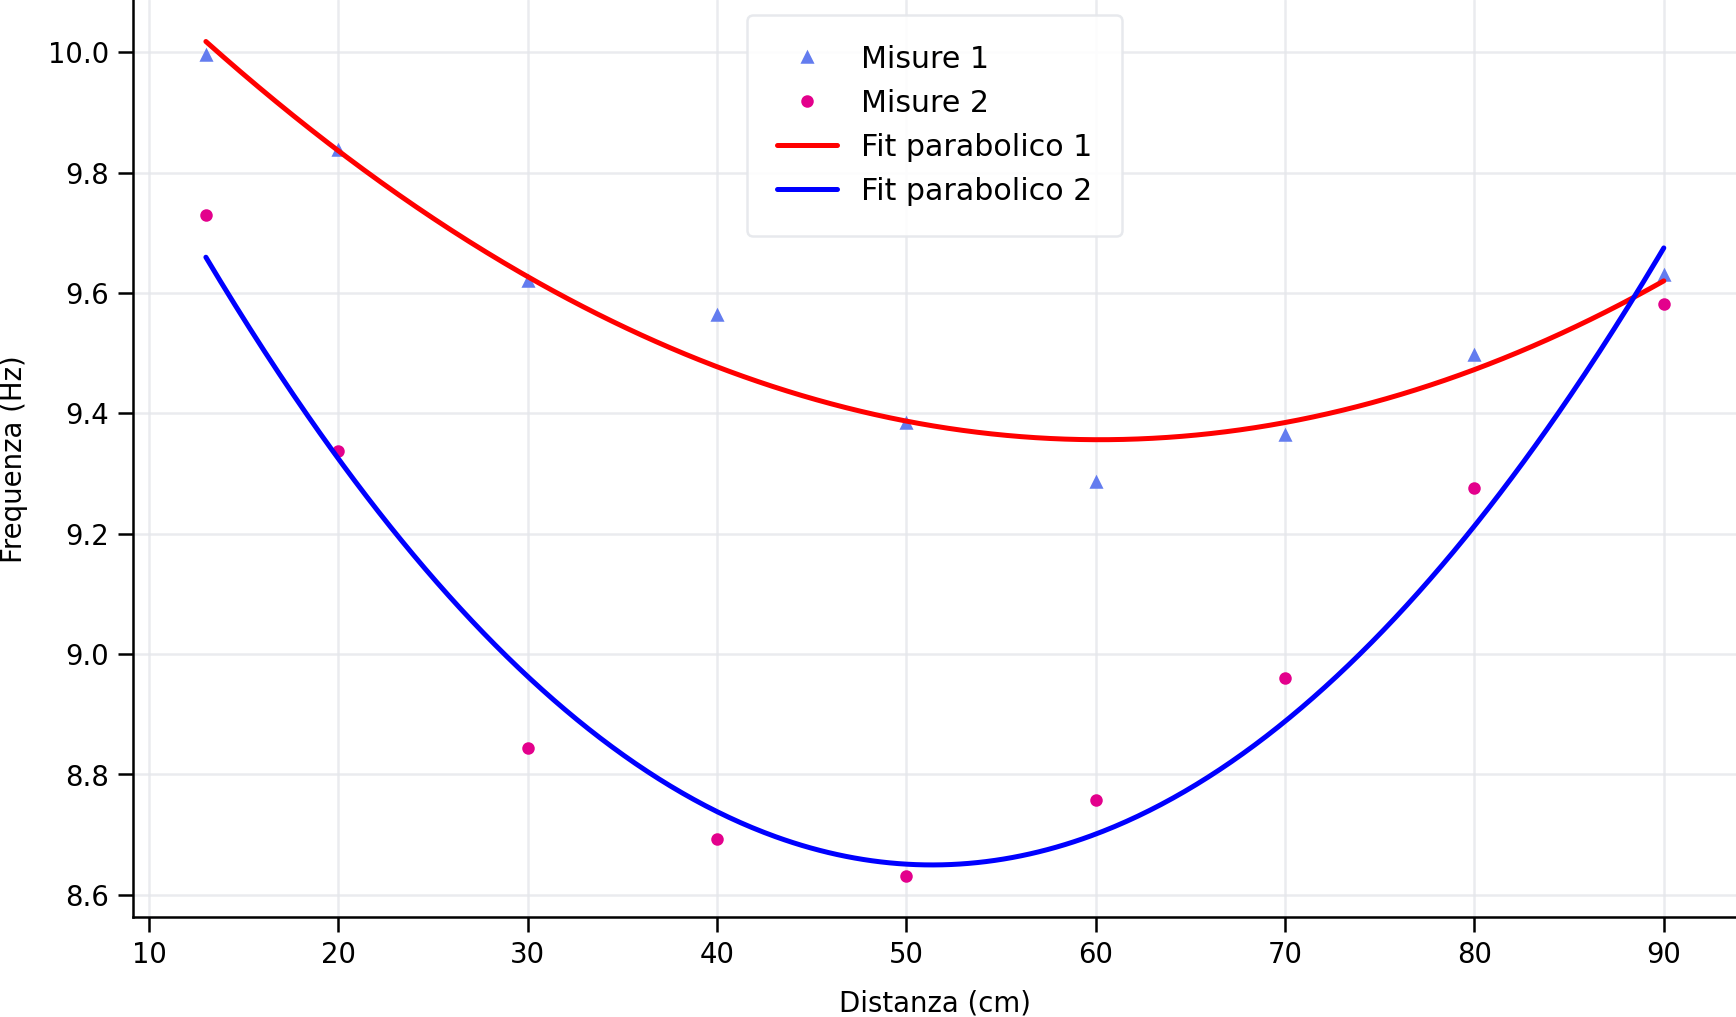
\includegraphics[width=.82\textwidth]{fig_fit_scipy.png}
\caption{Fit delle due serie mediante \texttt{scipy.optimize.curve\_fit}.}
\end{figure}

\section{Fit con \texttt{numpy.polyfit}}
\begin{lstlisting}
# Importa NumPy per lettura dati e regressione polinomiale.
import numpy as np

# Importa Matplotlib per la rappresentazione grafica.
import matplotlib.pyplot as plt

# Legge le tre colonne del file in tre array separati.
x, y1, y2 = np.loadtxt("Kter.txt", unpack=True)

# Esegue il fit di grado 2 della prima serie.
# p1 contiene i coefficienti [a, b, c].
p1 = np.polyfit(x, y1, 2)

# Esegue il fit di grado 2 della seconda serie.
p2 = np.polyfit(x, y2, 2)

# Genera una griglia fitta per disegnare curve regolari.
xfit = np.linspace(x.min(), x.max(), 500)

# Valuta il primo polinomio nei punti della griglia.
yfit1 = np.polyval(p1, xfit)

# Valuta il secondo polinomio nei punti della griglia.
yfit2 = np.polyval(p2, xfit)

# Disegna la prima serie di misure.
plt.plot(x, y1, "^", label="Misure 1")

# Disegna la seconda serie di misure.
plt.plot(x, y2, "o", label="Misure 2")

# Disegna in rosso il primo fit parabolico.
plt.plot(
    xfit, yfit1, "r-", lw=2,
    label="Fit parabolico 1",
)

# Disegna in blu il secondo fit parabolico.
plt.plot(
    xfit, yfit2, "b-", lw=2,
    label="Fit parabolico 2",
)

# Imposta l'etichetta dell'asse x.
plt.xlabel("Distanza (cm)")

# Imposta l'etichetta dell'asse y.
plt.ylabel("Frequenza (Hz)")

# Visualizza la legenda.
plt.legend()

# Salva la figura in formato vettoriale PDF.
plt.savefig("grafico.pdf")

# Salva la figura in formato PNG ad alta risoluzione.
plt.savefig("grafico.png", dpi=300)

# Visualizza la figura.
plt.show()
\end{lstlisting}

\subsection{Metodo dei minimi quadrati in NumPy}
\texttt{np.polyfit(x,y,2)} costruisce un polinomio di grado 2 e restituisce i coefficienti che minimizzano la somma dei quadrati dei residui. Il problema viene scritto nella forma matriciale
\[
 \mathbf{A}\mathbf{p}\simeq\mathbf{y},
\]
dove
\[
 \mathbf{A}=
 \begin{pmatrix}
 x_1^2 & x_1 & 1\\
 x_2^2 & x_2 & 1\\
 \vdots & \vdots & \vdots\\
 x_N^2 & x_N & 1
 \end{pmatrix},
 \qquad
 \mathbf{p}=
 \begin{pmatrix}a\\b\\c\end{pmatrix}.
\]
La matrice $\mathbf{A}$ è una matrice di Vandermonde. NumPy risolve il problema lineare ai minimi quadrati usando una decomposizione numerica collegata alla SVD, evitando di calcolare esplicitamente l'inversa di $\mathbf{A}^{T}\mathbf{A}$.

Il valore \texttt{2} è il grado del polinomio. I coefficienti sono ordinati dalla potenza più alta alla più bassa:
\[
 \texttt{p1[0]}=a,\qquad
 \texttt{p1[1]}=b,\qquad
 \texttt{p1[2]}=c.
\]
\texttt{np.polyval(p1,xfit)} valuta il polinomio nei punti della griglia \texttt{xfit}.

\subsection{Fit pesato con NumPy}
Se sono disponibili le incertezze $\sigma_i$ sulle ordinate, si può usare
\begin{lstlisting}
p = np.polyfit(x, y, 2, w=1/yerr)
\end{lstlisting}
I pesi di \texttt{polyfit} moltiplicano i residui non elevati al quadrato. Per ottenere il consueto chi-quadro, il peso corretto è quindi $w_i=1/\sigma_i$, non $1/\sigma_i^2$.



\section{Fit con NumPy e matrice di covarianza}
\begin{lstlisting}
# Importa NumPy per calcolo numerico e fit polinomiale.
import numpy as np

# Importa Matplotlib per costruire la figura.
import matplotlib.pyplot as plt

# Legge le tre colonne come array x, y1 e y2.
x, y1, y2 = np.loadtxt("Kter.txt", unpack=True)

# Esegue il fit quadratico della prima serie.
# cov=True richiede anche la matrice di covarianza.
p1, cov1 = np.polyfit(x, y1, 2, cov=True)

# Esegue il fit e calcola la covarianza della seconda serie.
p2, cov2 = np.polyfit(x, y2, 2, cov=True)

# Estrae le varianze di a, b, c e ne calcola la radice.
err1 = np.sqrt(np.diag(cov1))

# Calcola le incertezze standard del secondo fit.
err2 = np.sqrt(np.diag(cov2))

# Costruisce una griglia di 500 punti per le curve.
xfit = np.linspace(x.min(), x.max(), 500)

# Valuta il primo polinomio sulla griglia.
yfit1 = np.polyval(p1, xfit)

# Valuta il secondo polinomio sulla griglia.
yfit2 = np.polyval(p2, xfit)

# Disegna i dati della prima serie.
plt.plot(x, y1, "^", label="Misure 1")

# Disegna i dati della seconda serie.
plt.plot(x, y2, "o", label="Misure 2")

# Disegna la curva del primo fit.
plt.plot(
    xfit, yfit1, "r-", lw=2,
    label="Fit parabolico 1",
)

# Disegna la curva del secondo fit.
plt.plot(
    xfit, yfit2, "b-", lw=2,
    label="Fit parabolico 2",
)

# Imposta l'etichetta dell'asse orizzontale.
plt.xlabel("Distanza (cm)")

# Imposta l'etichetta dell'asse verticale.
plt.ylabel("Frequenza (Hz)")

# Costruisce la legenda.
plt.legend()

# Stampa un'intestazione per i risultati del primo fit.
print("\nFit 1")

# Stampa a con cinque cifre significative e il suo errore.
print(f"a = {p1[0]:.5g} +/- {err1[0]:.2g}")

# Stampa b e la relativa incertezza.
print(f"b = {p1[1]:.5g} +/- {err1[1]:.2g}")

# Stampa c e la relativa incertezza.
print(f"c = {p1[2]:.5g} +/- {err1[2]:.2g}")

# Stampa un'intestazione per i risultati del secondo fit.
print("\nFit 2")

# Stampa a e la sua incertezza per il secondo fit.
print(f"a = {p2[0]:.5g} +/- {err2[0]:.2g}")

# Stampa b e la sua incertezza per il secondo fit.
print(f"b = {p2[1]:.5g} +/- {err2[1]:.2g}")

# Stampa c e la sua incertezza per il secondo fit.
print(f"c = {p2[2]:.5g} +/- {err2[2]:.2g}")

# Salva la figura in formato PDF vettoriale.
plt.savefig("grafico.pdf")

# Salva la figura in formato PNG a 300 dpi.
plt.savefig("grafico.png", dpi=300)

# Visualizza la figura.
plt.show()
\end{lstlisting}

\section{Significato della matrice di covarianza}
La matrice di covarianza dei parametri è, nel caso di tre parametri,
\[
 \mathbf{C}=
 \begin{pmatrix}
 \operatorname{Var}(a) & \operatorname{Cov}(a,b) & \operatorname{Cov}(a,c)\\
 \operatorname{Cov}(b,a) & \operatorname{Var}(b) & \operatorname{Cov}(b,c)\\
 \operatorname{Cov}(c,a) & \operatorname{Cov}(c,b) & \operatorname{Var}(c)
 \end{pmatrix}.
\]
Essa descrive sia le incertezze individuali dei parametri sia le loro correlazioni statistiche.

Gli elementi diagonali sono le varianze stimate:
\[
 C_{aa}=\sigma_a^2,\qquad
 C_{bb}=\sigma_b^2,\qquad
 C_{cc}=\sigma_c^2.
\]
Per questo motivo le incertezze standard si ricavano mediante
\begin{lstlisting}
err = np.sqrt(np.diag(cov))
\end{lstlisting}
Gli elementi fuori diagonale sono covarianze. Una covarianza diversa da zero indica che le variazioni ammissibili di due parametri non sono indipendenti. In un fit parabolico, per esempio, una variazione del coefficiente quadratico può essere parzialmente compensata da una variazione del coefficiente lineare o del termine costante.

La matrice è utile per:
\begin{itemize}
  \item riportare correttamente le incertezze sui parametri;
  \item valutare le correlazioni tra i parametri;
  \item propagare le incertezze a una quantità dipendente dai parametri;
  \item costruire bande di incertezza della funzione di fit;
  \item riconoscere fit mal condizionati, nei quali alcuni parametri risultano fortemente correlati.
\end{itemize}

La correlazione normalizzata tra due parametri $p_i$ e $p_j$ è
\[
 \rho_{ij}=\frac{C_{ij}}{\sqrt{C_{ii}C_{jj}}},
\]
con valori compresi tra $-1$ e $+1$. Valori in modulo vicini a uno indicano una forte correlazione o anticorrelazione.

In \texttt{np.polyfit(...,cov=True)}, la covarianza è normalmente scalata in modo che il chi-quadro ridotto sia unitario. Se si forniscono pesi derivati da incertezze assolute affidabili, si può richiedere
\begin{lstlisting}
p, cov = np.polyfit(
    x, y, 2,
    w=1/yerr,
    cov="unscaled",
)
\end{lstlisting}
In \texttt{curve\_fit}, il ruolo analogo è svolto dall'opzione \texttt{absolute\_sigma=True}.

\section{Propagazione della covarianza alla curva di fit}
Il valore della parabola in un punto $x$ può essere scritto come
\[
 f(x)=\mathbf{v}^{T}\mathbf{p},
 \qquad
 \mathbf{v}=\begin{pmatrix}x^2\\x\\1\end{pmatrix}.
\]
La varianza propagata della curva è
\[
 \sigma_f^2(x)=\mathbf{v}^{T}\mathbf{C}\mathbf{v}.
\]
In Python si può calcolare una banda di incertezza con:
\begin{lstlisting}
V = np.column_stack((xfit**2, xfit, np.ones_like(xfit)))
var_fit = np.einsum("ij,jk,ik->i", V, cov1, V)
sigma_fit = np.sqrt(var_fit)

plt.fill_between(
    xfit,
    yfit1 - sigma_fit,
    yfit1 + sigma_fit,
    alpha=0.25,
    label="Incertezza del fit",
)
\end{lstlisting}
Questa banda rappresenta l'incertezza associata ai parametri stimati e alle loro covarianze. Non coincide necessariamente con un intervallo di previsione per una nuova misura, che dovrebbe includere anche la dispersione sperimentale dei singoli dati.

\section{Confronto tra NumPy e SciPy}
\begin{center}
\begin{tabular}{p{.22\textwidth}p{.34\textwidth}p{.34\textwidth}}
\toprule
Aspetto & \texttt{numpy.polyfit} & \texttt{scipy.optimize.curve\_fit}\\
\midrule
Tipo di modello & Polinomio di grado assegnato & Funzione Python generica\\
Problema numerico & Minimi quadrati lineari nei coefficienti & Minimi quadrati non lineari in forma generale\\
Funzione obiettivo & Somma dei quadrati, eventualmente pesata & Chi-quadro con \texttt{sigma}; caso non pesato se \texttt{sigma=None}\\
Valori iniziali & Non richiesti & Utili o necessari per modelli non lineari complessi\\
Risultato & Coefficienti polinomiali & Parametri nell'ordine della funzione\\
Covarianza & Con \texttt{cov=True} & Restituita come \texttt{pcov}\\
Pesi & \texttt{w=1/sigma} & \texttt{sigma=sigma}\\
Uso tipico & Regressioni polinomiali & Modelli generici, anche non lineari\\
\bottomrule
\end{tabular}
\end{center}

È importante non contrapporre rigidamente ``minimi quadrati'' e ``chi-quadro'': il chi-quadro è una somma di residui quadratici normalizzati dalle incertezze. NumPy e SciPy appartengono quindi alla stessa famiglia concettuale. La differenza principale è che \texttt{polyfit} sfrutta la linearità del polinomio rispetto ai coefficienti e risolve direttamente un problema lineare, mentre \texttt{curve\_fit} usa un algoritmo iterativo generale per minimizzare la funzione obiettivo.

Nel caso della parabola e in assenza di pesi, i due metodi devono fornire risultati compatibili entro la precisione numerica. Le differenze diventano sostanziali quando il modello non è lineare nei parametri, quando si introducono vincoli oppure quando sono necessari valori iniziali.

\section{Stampa corretta dei parametri}
La sintassi
\begin{lstlisting}
print(f"a = {p1[0]:.5g} +/- {err1[0]:.2g}")
\end{lstlisting}
usa una f-string. L'espressione \texttt{p1[0]} seleziona il parametro, mentre \texttt{:.5g} richiede cinque cifre significative. Analogamente, \texttt{:.2g} richiede due cifre significative per l'incertezza.

Non devono comparire backslash all'interno delle parentesi quadre della f-string. Forme come \texttt{p1\textbackslash[0\textbackslash]} producono un errore sintattico. Inoltre, il formato deve essere applicato all'elemento dell'array e non all'array stesso.

\begin{figure}[H]
\centering
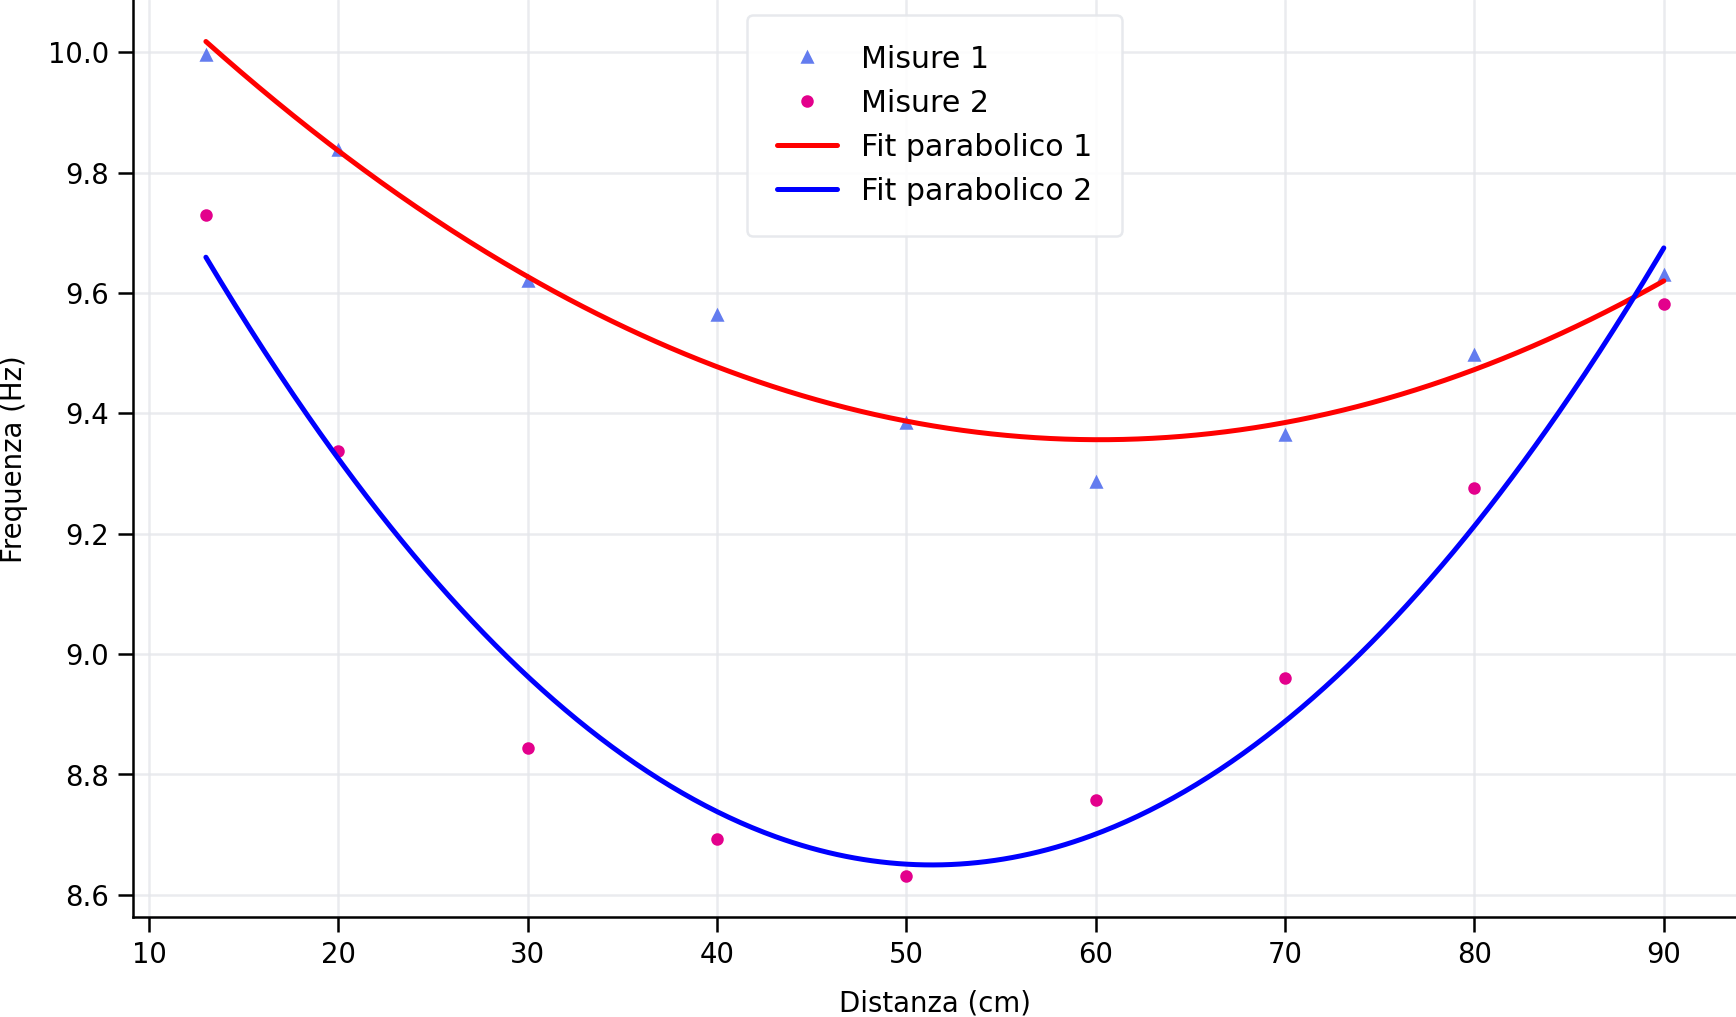
\includegraphics[width=.82\textwidth]{fig_fit_numpy.png}
\caption{Fit parabolico ottenuto con \texttt{numpy.polyfit} e valutato con \texttt{numpy.polyval}.}
\end{figure}


\section{Buone pratiche conclusive}
\begin{itemize}
  \item mantenere coerenti i nomi dei file negli script e nella cartella di lavoro;
  \item indicare sempre grandezze e unità sugli assi;
  \item distinguere serie diverse mediante marker oltre che mediante colori;
  \item usare l'interfaccia \texttt{fig, ax} per figure complesse o con più pannelli;
  \item rappresentare le incertezze sperimentali quando sono disponibili;
  \item salvare la figura prima di chiamare \texttt{show()};
  \item usare PDF per la grafica vettoriale e PNG ad alta risoluzione per la grafica raster;
  \item usare un fit pesato quando le incertezze dei punti non sono uguali;
  \item riportare parametri, incertezze, covarianze e un indicatore della qualità del fit;
  \item controllare i residui, perché un valore accettabile del chi-quadro non sostituisce l'ispezione dell'andamento sistematico degli scarti.
\end{itemize}


\chapter{Istogrammi e fit con Python}
\label{chap:istogrammi-fit}

\section{Introduzione}

Un istogramma rappresenta la distribuzione di un insieme di dati numerici.
L'intervallo compreso tra il valore minimo e il valore massimo viene
suddiviso in sottointervalli, detti \emph{bin}. Per ogni bin si conta il
numero di dati che ricadono al suo interno.

Se indichiamo con $N_i$ il numero di elementi contenuti nel bin $i$,
l'istogramma è costituito dalla sequenza dei conteggi

\[
N_1,N_2,\ldots,N_m,
\]

dove $m$ è il numero complessivo dei bin.

L'altezza di ciascuna barra rappresenta quindi una frequenza assoluta.
L'asse orizzontale riporta i valori della variabile osservata, mentre
l'asse verticale riporta il numero di osservazioni contenute in ciascun
intervallo.

In questo capitolo si costruirà un istogramma per gradi:

\begin{enumerate}
    \item calcolo manuale dei conteggi;
    \item uso elementare di \texttt{plt.hist};
    \item aggiunta delle etichette degli assi;
    \item scelta del numero di bin e personalizzazione grafica;
    \item recupero dei conteggi e dei bordi dei bin;
    \item sovrapposizione di un fit gaussiano.
\end{enumerate}

\section{Costruzione manuale: \texttt{istogrammamimano.py}}

Il primo script costruisce i conteggi senza utilizzare NumPy o
Matplotlib per il calcolo dell'istogramma.

\begin{lstlisting}[language=Python]
def istogrammello(data, div):
    high = max(data) + 0.01
    low = min(data) - 0.01
    delta = (high - low) / div

    hist = []

    for a in range(div):
        hist.append(0.)

    for a in data:
        for b in range(div):
            if a > low + b*delta and a <= low + (b+1)*delta:
                hist[b] = hist[b] + 1

    return hist


dati = list(
    map(
        float,
        open("daterelli.dat").read().strip().split()
    )
)

histo = istogrammello(dati, 10)

for a in histo:
    print(a)
\end{lstlisting}

\subsection{Argomenti della funzione}

La funzione

\begin{lstlisting}[language=Python]
def istogrammello(data, div):
\end{lstlisting}

riceve due argomenti:

\begin{itemize}
    \item \texttt{data}: la sequenza dei dati numerici;
    \item \texttt{div}: il numero di intervalli nei quali dividere il
          campo dei dati.
\end{itemize}

\subsection{Estremi dell'intervallo}

Le istruzioni

\begin{lstlisting}[language=Python]
high = max(data) + 0.01
low = min(data) - 0.01
\end{lstlisting}

calcolano gli estremi superiore e inferiore. Il piccolo margine aggiunto
agli estremi riduce il rischio che il valore minimo o massimo rimanga
escluso a causa delle disuguaglianze usate nella selezione.

La larghezza comune dei bin è

\[
\Delta = \frac{x_{\max}-x_{\min}}{m},
\]

ed è calcolata da

\begin{lstlisting}[language=Python]
delta = (high - low) / div
\end{lstlisting}

Tutti i bin hanno quindi la stessa larghezza.

\subsection{Inizializzazione dei conteggi}

La lista dei conteggi è inizialmente vuota:

\begin{lstlisting}[language=Python]
hist = []
\end{lstlisting}

Il primo ciclo inserisce un valore nullo per ogni bin:

\begin{lstlisting}[language=Python]
for a in range(div):
    hist.append(0.)
\end{lstlisting}

Se \texttt{div=10}, al termine del ciclo la lista contiene dieci zeri.
Il valore \texttt{hist[b]} memorizzerà il numero di dati appartenenti al
bin $b$.

\subsection{Assegnazione dei dati ai bin}

Il doppio ciclo

\begin{lstlisting}[language=Python]
for a in data:
    for b in range(div):
\end{lstlisting}

considera ogni dato \texttt{a} e controlla tutti i bin. Il dato appartiene
al bin $b$ se soddisfa

\[
x_{\min}+b\Delta < a
\leq x_{\min}+(b+1)\Delta.
\]

Nel codice:

\begin{lstlisting}[language=Python]
if a > low + b*delta and a <= low + (b+1)*delta:
    hist[b] = hist[b] + 1
\end{lstlisting}

Quando la condizione è vera, il conteggio del bin viene incrementato di
uno.

\begin{figure}[htbp]
\centering
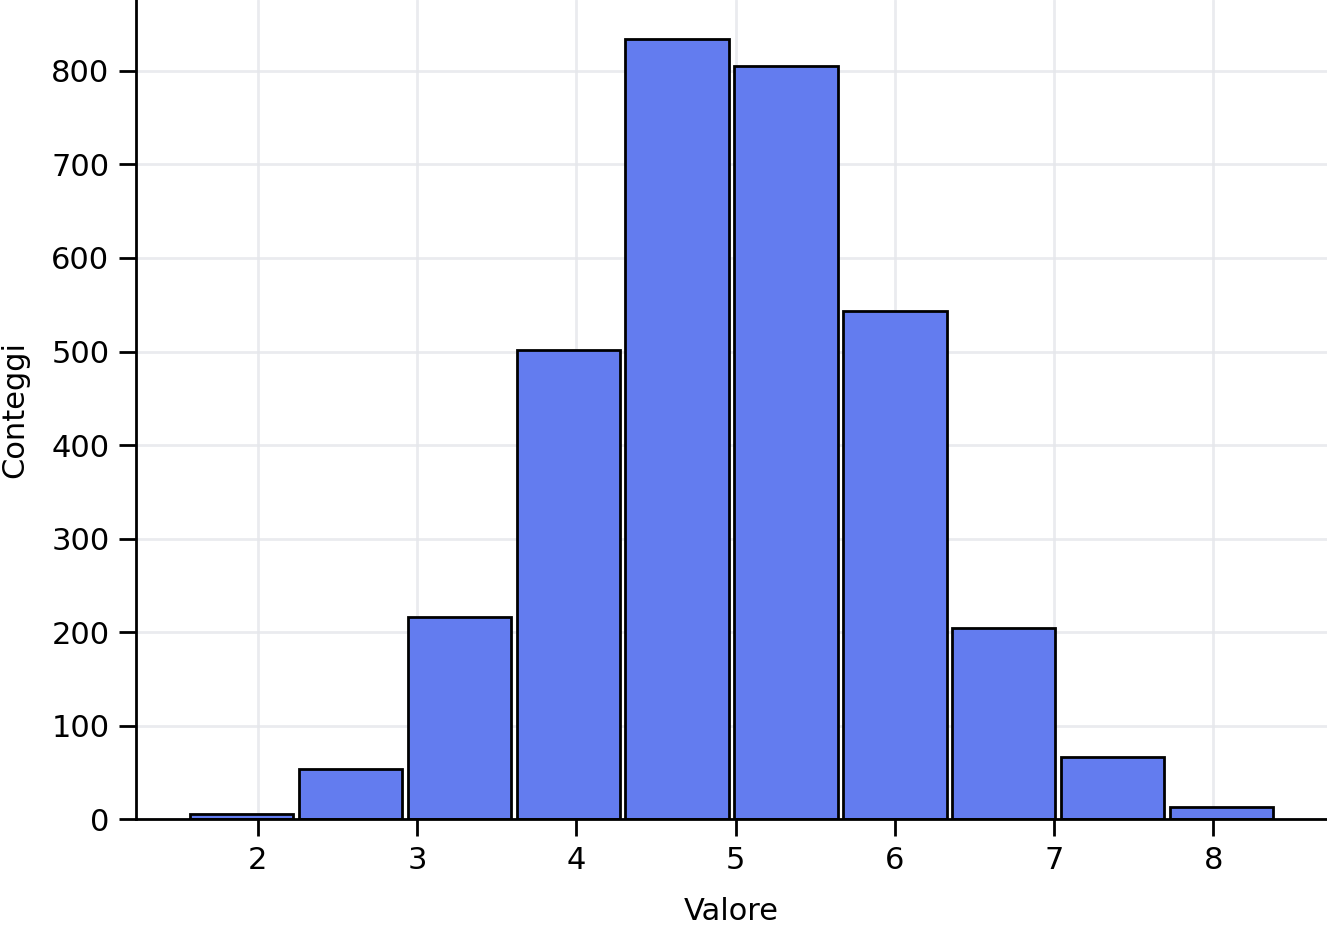
\includegraphics[width=0.78\textwidth]{fig_istogramma_manuale.png}
\caption{Rappresentazione grafica dei conteggi calcolati manualmente da \texttt{istogrammamimano.py}.}
\label{fig:istogramma-manuale}
\end{figure}

Questo algoritmo è didatticamente utile perché mostra come nasce un
istogramma. Non è però efficiente: per $N$ dati e $m$ bin esegue fino a
$N\times m$ confronti. Inoltre produce soltanto i conteggi, non una
figura.

\subsection{Lettura manuale del file}

L'espressione

\begin{lstlisting}[language=Python]
open("daterelli.dat").read().strip().split()
\end{lstlisting}

apre il file, legge tutto il contenuto, elimina gli spazi iniziali e
finali e separa il testo in singole stringhe. Successivamente,

\begin{lstlisting}[language=Python]
map(float, ...)
\end{lstlisting}

converte ogni stringa in un numero reale, mentre \texttt{list} costruisce
la lista finale.

Nel materiale disponibile il file dei dati è denominato
\texttt{daterelli.txt}. Per eseguire lo script nella stessa cartella del
file fornito, occorre quindi rendere coerente il nome:

\begin{lstlisting}[language=Python]
open("daterelli.txt")
\end{lstlisting}

\section{Primo istogramma con Matplotlib: \texttt{istogrammami.py}}

Il secondo script affida a NumPy la lettura dei dati e a Matplotlib il
calcolo e la visualizzazione dell'istogramma.

\begin{lstlisting}[language=Python]
import numpy as np
import matplotlib.pyplot as plt

x = np.loadtxt("daterelli.dat")

plt.hist(x)
plt.show()
\end{lstlisting}

\subsection{Lettura con \texttt{np.loadtxt}}

L'istruzione

\begin{lstlisting}[language=Python]
x = np.loadtxt("daterelli.dat")
\end{lstlisting}

legge i valori numerici e restituisce un array NumPy. Anche in questo
script il nome deve essere sostituito con \texttt{daterelli.txt} se si
usa il file allegato.

Rispetto alla lettura manuale, \texttt{np.loadtxt} rende il codice più
breve e restituisce direttamente una struttura adeguata al calcolo
numerico.

\subsection{Il ruolo di \texttt{plt.hist}}

La chiamata

\begin{lstlisting}[language=Python]
plt.hist(x)
\end{lstlisting}

svolge due operazioni:

\begin{enumerate}
    \item calcola la suddivisione in bin e i relativi conteggi;
    \item disegna le barre dell'istogramma.
\end{enumerate}

\begin{figure}[htbp]
\centering
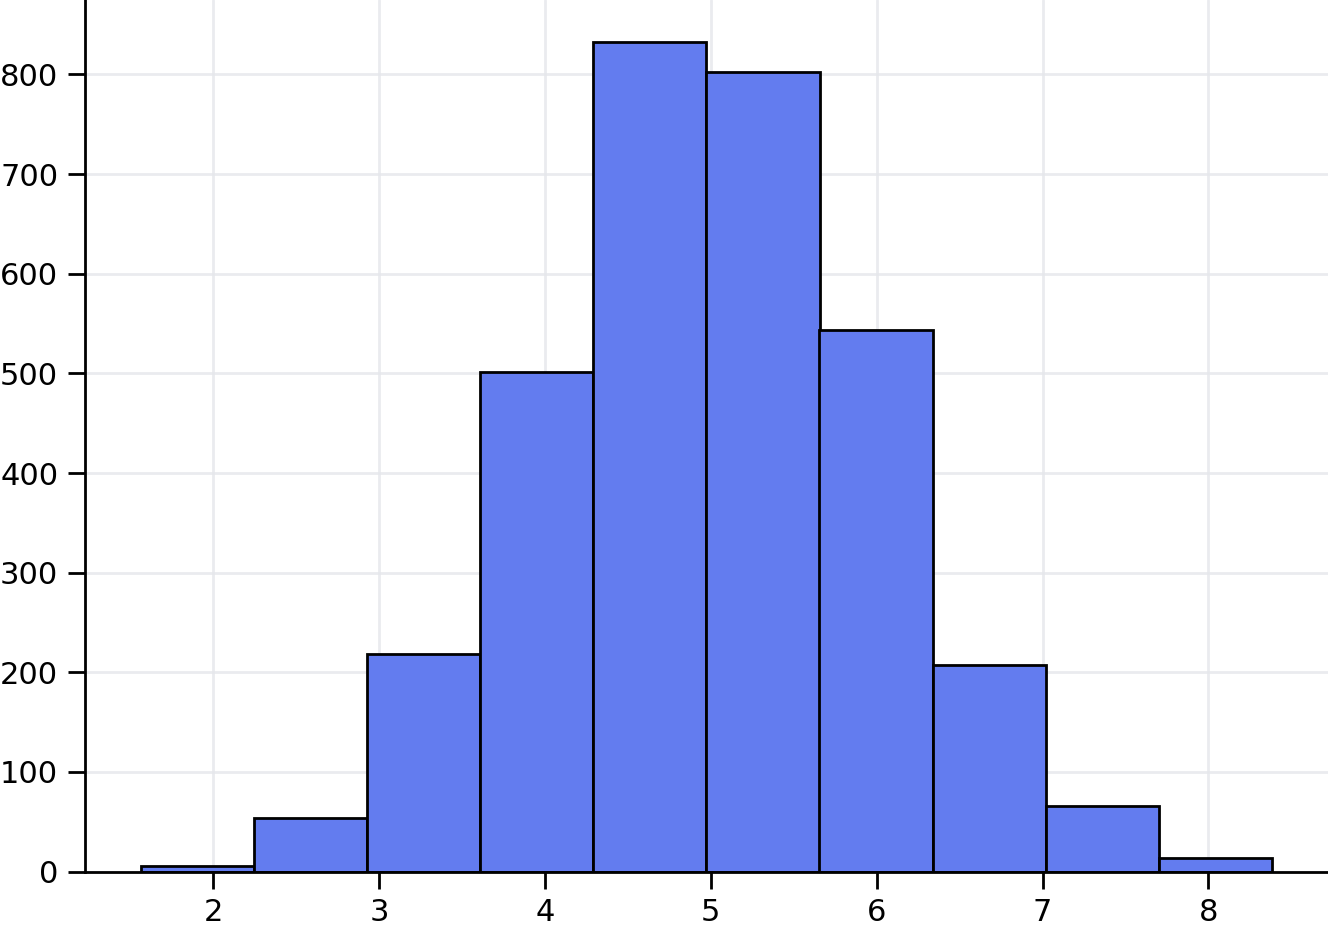
\includegraphics[width=0.78\textwidth]{fig_istogrammami.png}
\caption{Istogramma minimo prodotto da \texttt{istogrammami.py}.}
\label{fig:istogrammami}
\end{figure}

Quando il numero di bin non è specificato, viene utilizzato il valore
predefinito di Matplotlib. Questo script è adatto a un controllo rapido
della distribuzione, ma non documenta ancora le grandezze sugli assi.

\section{Aggiunta delle etichette: \texttt{istogrammami2.py}}

\begin{lstlisting}[language=Python]
import numpy as np
import matplotlib.pyplot as plt

x = np.loadtxt("daterelli.dat")

plt.hist(x)
plt.xlabel("Valore")
plt.ylabel("Conteggi")
plt.show()
\end{lstlisting}

Le istruzioni

\begin{lstlisting}[language=Python]
plt.xlabel("Valore")
plt.ylabel("Conteggi")
\end{lstlisting}

aggiungono rispettivamente il nome dell'asse orizzontale e dell'asse
verticale.

\begin{figure}[htbp]
\centering
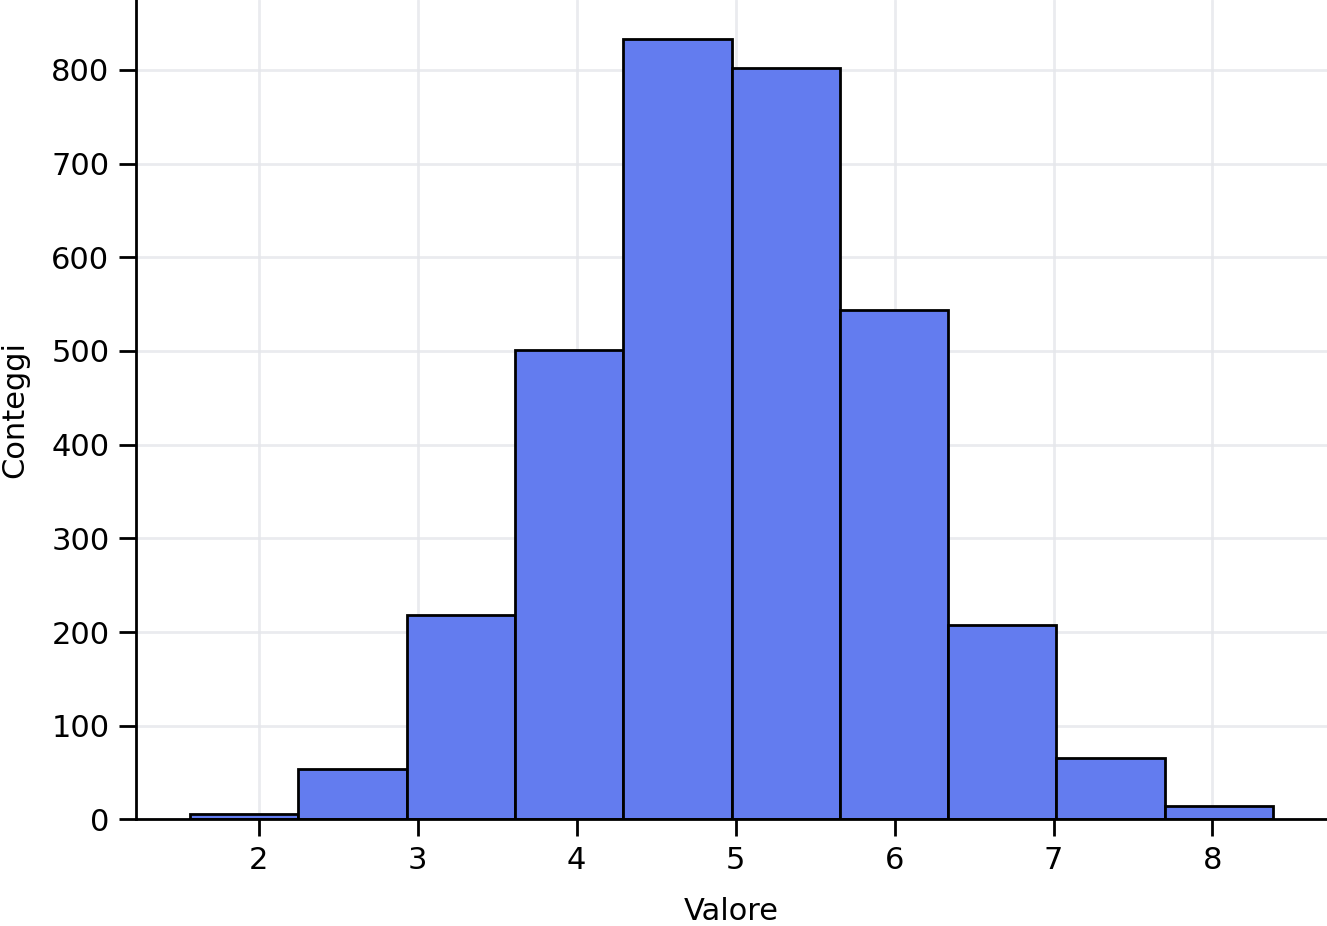
\includegraphics[width=0.78\textwidth]{fig_istogrammami2.png}
\caption{Istogramma con etichette degli assi prodotto da \texttt{istogrammami2.py}.}
\label{fig:istogrammami2}
\end{figure}

La parola \texttt{Conteggi} chiarisce che l'altezza dei bin rappresenta
il numero assoluto di dati. Se si usasse un istogramma normalizzato,
l'etichetta dovrebbe essere modificata, per esempio in
\texttt{Densita di probabilita}.

In una figura scientifica è opportuno specificare anche l'unità di
misura della variabile rappresentata, quando esiste. Per esempio:

\begin{lstlisting}[language=Python]
plt.xlabel("Energia (MeV)")
\end{lstlisting}

\section{Numero di bin e stile: \texttt{istogrammami3.py}}

\begin{lstlisting}[language=Python]
import numpy as np
import matplotlib.pyplot as plt

x = np.loadtxt("daterelli.txt")

plt.hist(
    x,
    bins=20,
    color="skyblue",
    edgecolor="black"
)

plt.xlabel("Valore")
plt.ylabel("Conteggi")
plt.show()
plt.savefig("grafico.pdf")
\end{lstlisting}

\begin{figure}[htbp]
\centering
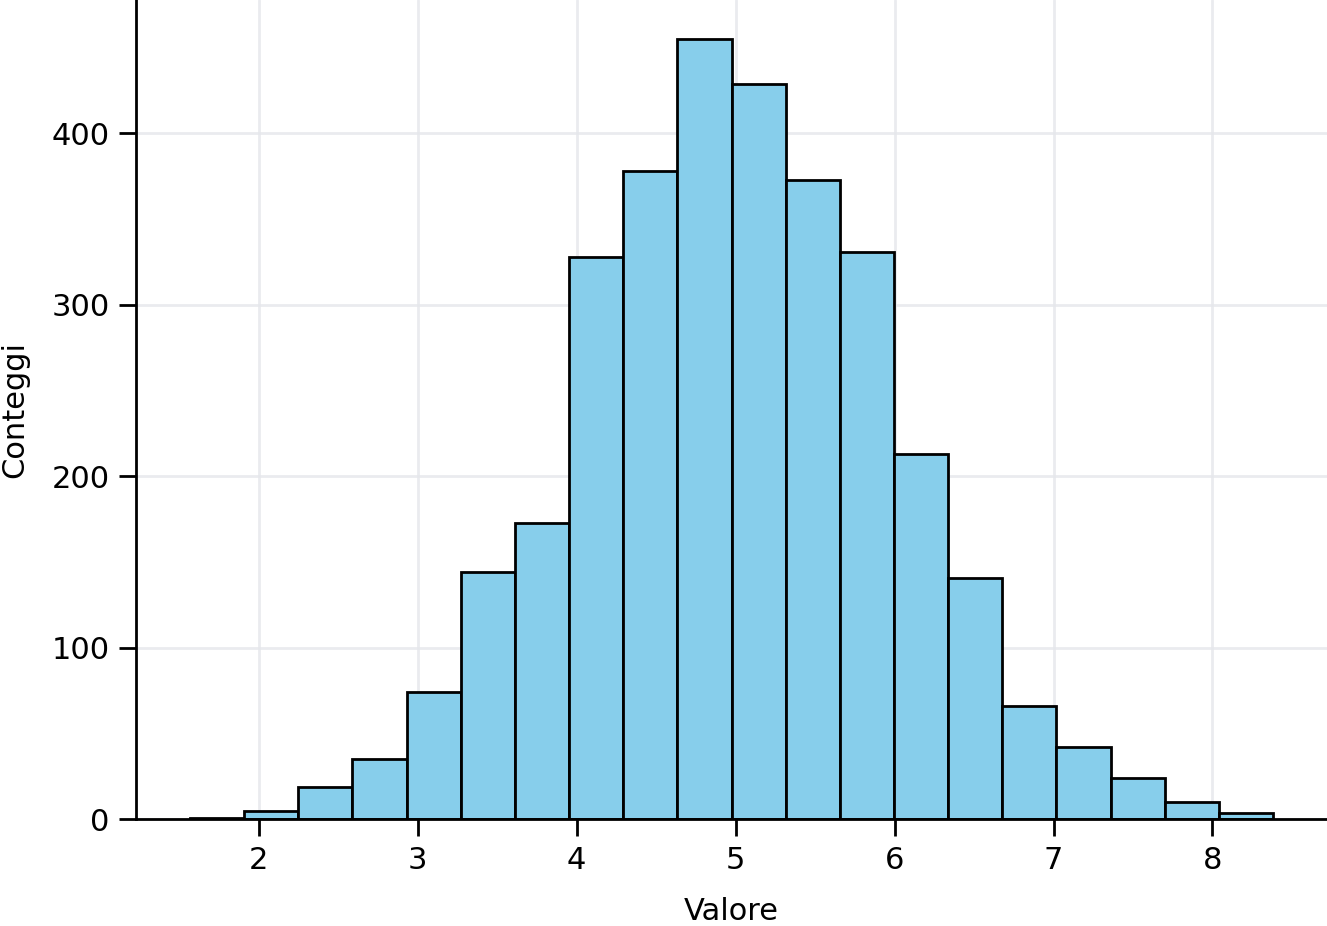
\includegraphics[width=0.78\textwidth]{fig_istogrammami3.png}
\caption{Istogramma a 20 bin con riempimento azzurro e bordi neri.}
\label{fig:istogrammami3}
\end{figure}

\subsection{Scelta del numero di bin}

L'opzione

\begin{lstlisting}[language=Python]
bins=20
\end{lstlisting}

suddivide il campo dei dati in 20 intervalli. La scelta del numero di bin
influenza l'aspetto della distribuzione:

\begin{itemize}
    \item pochi bin producono una rappresentazione molto regolare, ma
          possono nascondere dettagli;
    \item molti bin mostrano più dettagli, ma aumentano le fluttuazioni
          statistiche dei conteggi;
    \item il risultato del successivo fit può dipendere dalla scelta dei
          bin, perché il fit viene effettuato sui conteggi raggruppati.
\end{itemize}

\subsection{Colore e bordi}

L'opzione

\begin{lstlisting}[language=Python]
color="skyblue"
\end{lstlisting}

imposta il colore interno delle barre. L'opzione

\begin{lstlisting}[language=Python]
edgecolor="black"
\end{lstlisting}

rende neri i bordi, migliorando la separazione visiva tra bin
consecutivi.

\subsection{Salvataggio della figura}

Lo script usa

\begin{lstlisting}[language=Python]
plt.savefig("grafico.pdf")
\end{lstlisting}

per salvare la figura in PDF. È preferibile salvare la figura prima di
\texttt{plt.show()}:

\begin{lstlisting}[language=Python]
plt.savefig("grafico.pdf")
plt.show()
\end{lstlisting}

Alcuni backend possono infatti modificare o chiudere la figura corrente
dopo la visualizzazione.


\section{Istogrammi delle frequenze relative}
\label{sec:frequenze-relative}

\subsection{Frequenze assolute e frequenze relative}

Un istogramma delle frequenze assolute riporta, per ogni bin $i$, il
numero di osservazioni $N_i$ che ricadono nell'intervallo corrispondente.
La somma dei conteggi di tutti i bin coincide con il numero complessivo
dei dati:

\begin{equation}
N_{\mathrm{tot}}=\sum_i N_i.
\end{equation}

Se l'array \texttt{x} contiene tutti i dati, il numero totale delle
osservazioni è restituito da

\begin{lstlisting}[language=Python]
len(x)
\end{lstlisting}

La frequenza relativa del bin $i$ è definita come

\begin{equation}
f_i=\frac{N_i}{N_{\mathrm{tot}}}.
\end{equation}

Di conseguenza,

\begin{equation}
\sum_i f_i=1.
\end{equation}

Non bisogna dividere i conteggi per \texttt{sum(x)}, perché
\texttt{sum(x)} rappresenta la somma dei valori misurati e non il numero
totale delle osservazioni. Sono invece equivalenti, quando tutti i dati
ricadono nell'intervallo dell'istogramma,

\begin{lstlisting}[language=Python]
conteggi / len(x)
\end{lstlisting}

e

\begin{lstlisting}[language=Python]
conteggi / np.sum(conteggi)
\end{lstlisting}

\subsection{Calcolo esplicito delle frequenze relative}

Nel primo approccio l'istogramma assoluto è disegnato mediante
\texttt{plt.hist}, mentre le frequenze relative sono calcolate
esplicitamente a partire dai conteggi. Il codice è contenuto nello script
\texttt{frequenzarelative.py}.

\begin{lstlisting}[language=Python]
import numpy as np
import matplotlib.pyplot as plt

# lettura dati
x = np.loadtxt("daterelli.txt")

# =====================================================
# ISTOGRAMMA DELLE FREQUENZE ASSOLUTE
# =====================================================
plt.figure(figsize=(8, 6))

plt.hist(
    x,
    bins=20,
    color="skyblue",
    edgecolor="black"
)

plt.xlabel("Valore")
plt.ylabel("Conteggi")
plt.title("Frequenze assolute")
plt.savefig("istogramma_assoluto.pdf")
plt.show()

# =====================================================
# ISTOGRAMMA DELLE FREQUENZE RELATIVE
# =====================================================
conteggi, bin_edges = np.histogram(x, bins=20)

frequenze_relative = conteggi / len(x)

larghezze = np.diff(bin_edges)
centri = (bin_edges[:-1] + bin_edges[1:]) / 2

plt.figure(figsize=(8, 6))

plt.bar(
    centri,
    frequenze_relative,
    width=larghezze,
    color="lightgreen",
    edgecolor="black"
)

plt.xlabel("Valore")
plt.ylabel("Frequenza relativa")
plt.title("Frequenze relative")
plt.savefig("istogramma_relativo.pdf")
plt.show()
\end{lstlisting}

L'istruzione

\begin{lstlisting}[language=Python]
conteggi, bin_edges = np.histogram(x, bins=20)
\end{lstlisting}

calcola l'istogramma senza disegnarlo. L'array \texttt{conteggi}
contiene i valori $N_i$, mentre \texttt{bin\_edges} contiene i bordi
dei bin. Le frequenze relative sono quindi calcolate mediante

\begin{lstlisting}[language=Python]
frequenze_relative = conteggi / len(x)
\end{lstlisting}

Le larghezze e i centri dei bin sono necessari per disegnare il secondo
istogramma con \texttt{plt.bar}:

\begin{lstlisting}[language=Python]
larghezze = np.diff(bin_edges)
centri = (bin_edges[:-1] + bin_edges[1:]) / 2
\end{lstlisting}

Il vantaggio di questo approccio è didattico: il passaggio dai conteggi
$N_i$ alle frequenze relative $f_i$ è visibile esplicitamente nel
codice.

\begin{figure}[htbp]
    \centering
    \begin{minipage}{0.48\textwidth}
        \centering
        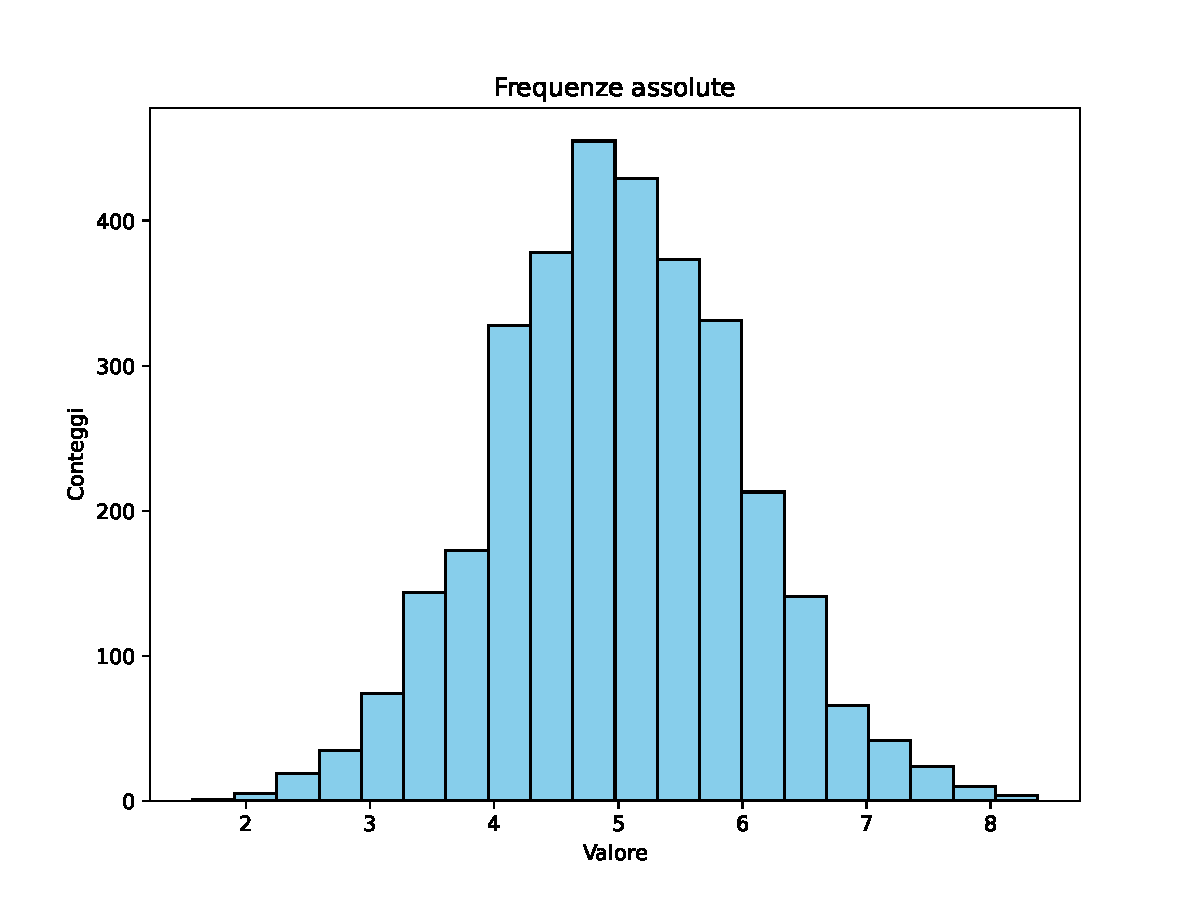
\includegraphics[width=\textwidth]{istogramma_assoluto.pdf}
        \caption*{(a) Frequenze assolute.}
    \end{minipage}
    \hfill
    \begin{minipage}{0.48\textwidth}
        \centering
        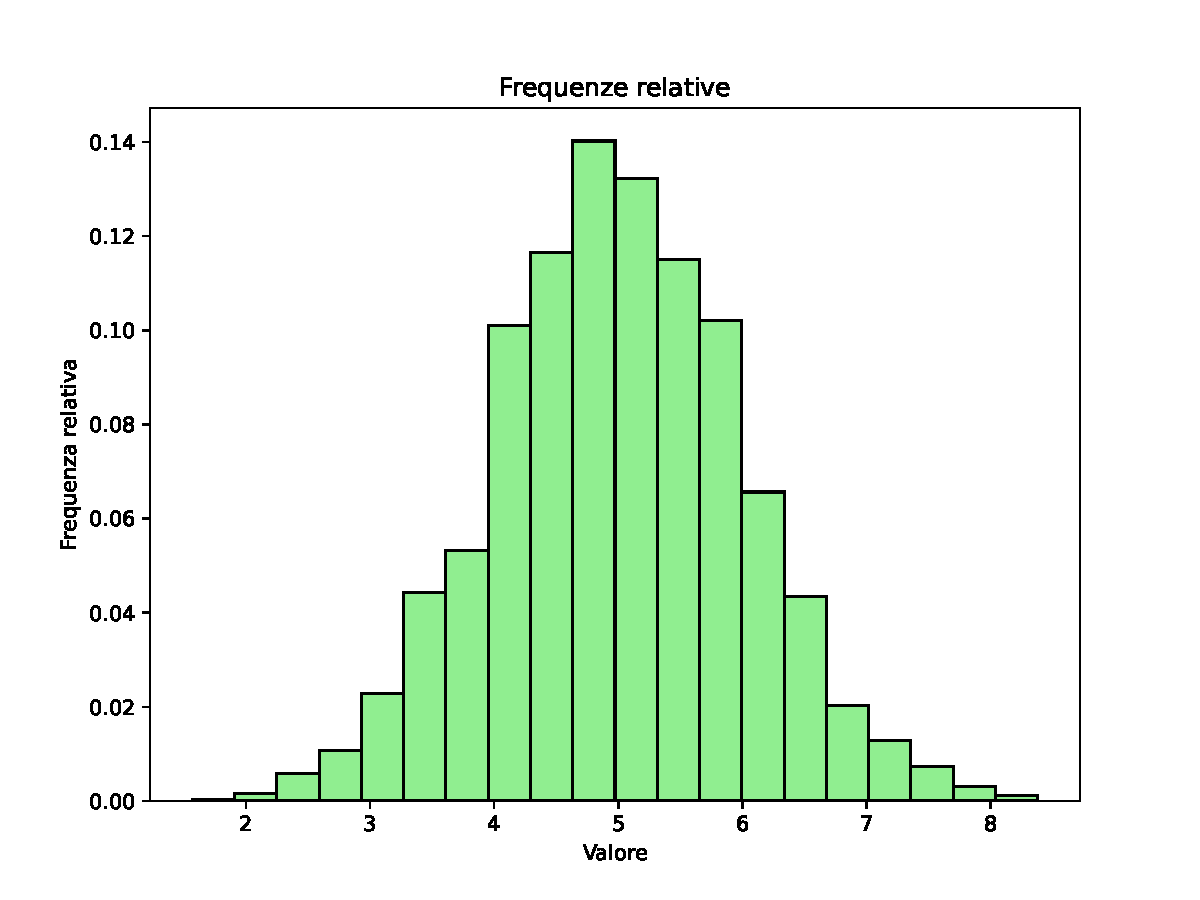
\includegraphics[width=\textwidth]{istogramma_relativo.pdf}
        \caption*{(b) Frequenze relative.}
    \end{minipage}
    \caption{Confronto tra l'istogramma dei conteggi e quello delle
    frequenze relative. I due grafici hanno la stessa forma, ma scale
    verticali differenti.}
    \label{fig:frequenze-assolute-relative}
\end{figure}

\subsection{Normalizzazione mediante i pesi di \texttt{plt.hist}}

Lo script \texttt{frequenzarelative2.py} costruisce direttamente
l'istogramma relativo con Matplotlib. A ogni osservazione viene assegnato
il peso

\begin{equation}
w=\frac{1}{N_{\mathrm{tot}}}.
\end{equation}

Poiché ogni dato contribuisce al proprio bin con $1/N_{\mathrm{tot}}$,
l'altezza del bin diventa automaticamente $N_i/N_{\mathrm{tot}}$.

\begin{lstlisting}[language=Python]
import numpy as np
import matplotlib.pyplot as plt

# lettura dati
x = np.loadtxt("daterelli.txt")

# =====================================================
# ISTOGRAMMA DELLE FREQUENZE ASSOLUTE
# =====================================================
plt.figure(figsize=(8, 6))

plt.hist(
    x,
    bins=20,
    color="skyblue",
    edgecolor="black"
)

plt.xlabel("Valore")
plt.ylabel("Conteggi")
plt.title("Frequenze assolute")
plt.savefig("istogramma_assoluto.pdf")
plt.show()

# =====================================================
# ISTOGRAMMA DELLE FREQUENZE RELATIVE
# =====================================================
plt.figure(figsize=(8, 6))

plt.hist(
    x,
    bins=20,
    weights=np.ones_like(x) / len(x),
    color="lightgreen",
    edgecolor="black"
)

plt.xlabel("Valore")
plt.ylabel("Frequenza relativa")
plt.title("Frequenze relative")
plt.savefig("istogramma_relativo.pdf")
plt.show()
\end{lstlisting}

L'istruzione

\begin{lstlisting}[language=Python]
np.ones_like(x)
\end{lstlisting}

crea un array di elementi uguali a 1 con la stessa forma di \texttt{x}.
La divisione per \texttt{len(x)} assegna quindi a ogni evento il peso
$1/N_{\mathrm{tot}}$:

\begin{lstlisting}[language=Python]
weights = np.ones_like(x) / len(x)
\end{lstlisting}

La somma dei pesi degli eventi contenuti nel bin $i$ è

\begin{equation}
\sum_{j\in i}\frac{1}{N_{\mathrm{tot}}}
=rac{N_i}{N_{\mathrm{tot}}}=f_i.
\end{equation}

Questa tecnica produce le frequenze relative direttamente con
\texttt{plt.hist}, senza calcolare separatamente centri e larghezze.

\subsection{Visualizzazione simultanea: una finestra o due finestre}

Gli script \texttt{frequenzarelative3.py} e
\texttt{frequenzarelative4.py} usano la stessa normalizzazione pesata,
ma organizzano diversamente la visualizzazione. Nel primo caso i due
grafici sono inseriti nella stessa figura; nel secondo caso sono creati
in due finestre indipendenti.

\subsubsection{Due pannelli nella stessa finestra}

Lo script \texttt{frequenzarelative3.py} crea una figura con una riga e
due colonne:

\begin{lstlisting}[language=Python]
import numpy as np
import matplotlib.pyplot as plt

# lettura dati
x = np.loadtxt("daterelli.txt")

# una figura con due pannelli affiancati
fig, ax = plt.subplots(1, 2, figsize=(12, 5))

# frequenze assolute nel pannello sinistro
ax[0].hist(
    x,
    bins=20,
    color="skyblue",
    edgecolor="black"
)

ax[0].set_xlabel("Valore")
ax[0].set_ylabel("Conteggi")
ax[0].set_title("Frequenze assolute")

# frequenze relative nel pannello destro
ax[1].hist(
    x,
    bins=20,
    weights=np.ones_like(x) / len(x),
    color="lightgreen",
    edgecolor="black"
)

ax[1].set_xlabel("Valore")
ax[1].set_ylabel("Frequenza relativa")
ax[1].set_title("Frequenze relative")

fig.tight_layout()

plt.savefig("istogrammi_confronto.pdf")
plt.savefig("istogrammi_confronto.png", dpi=300)
plt.show()
\end{lstlisting}

La chiamata

\begin{lstlisting}[language=Python]
fig, ax = plt.subplots(1, 2, figsize=(12, 5))
\end{lstlisting}

crea una sola finestra grafica contenente due oggetti \texttt{Axes}:
\texttt{ax[0]} è il pannello sinistro e \texttt{ax[1]} è il pannello
destro. Questa soluzione è particolarmente utile per il confronto
diretto, perché i due istogrammi sono visibili contemporaneamente e
rimangono allineati nella stessa figura.

\begin{figure}[htbp]
    \centering
    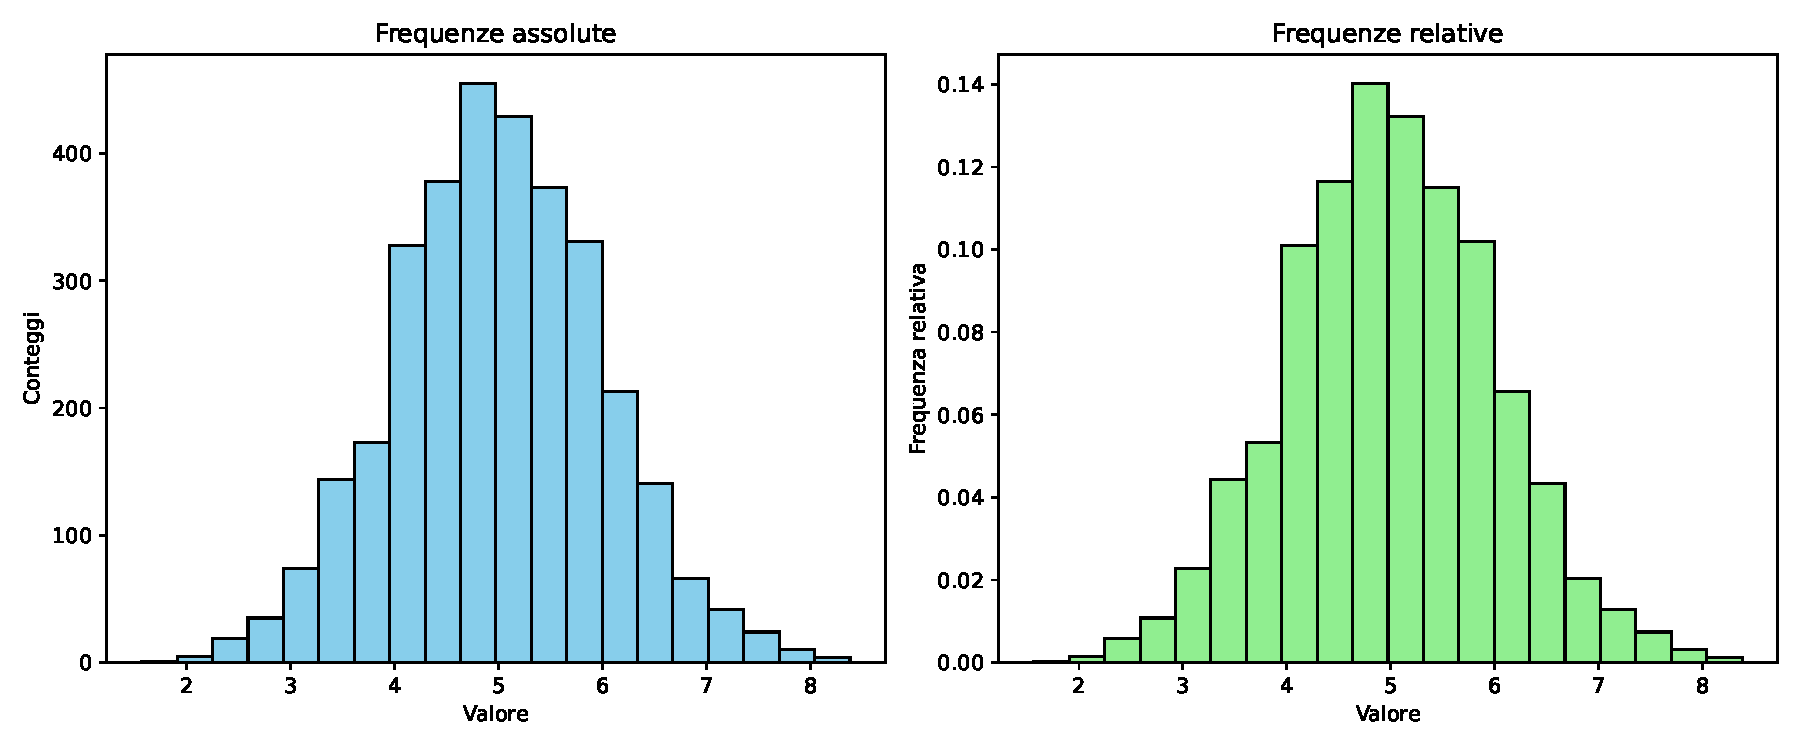
\includegraphics[width=\textwidth]{istogrammi_confronto.pdf}
    \caption{Frequenze assolute e relative rappresentate in due pannelli
    della stessa finestra.}
    \label{fig:istogrammi-confronto}
\end{figure}

\subsubsection{Due finestre grafiche indipendenti}

Lo script \texttt{frequenzarelative4.py} usa invece due chiamate
separate a \texttt{plt.figure}:

\begin{lstlisting}[language=Python]
import numpy as np
import matplotlib.pyplot as plt

# lettura dati
x = np.loadtxt("daterelli.txt")

# finestra 1: frequenze assolute
plt.figure("Frequenze assolute", figsize=(8, 6))

plt.hist(
    x,
    bins=20,
    color="skyblue",
    edgecolor="black"
)

plt.xlabel("Valore")
plt.ylabel("Conteggi")
plt.title("Frequenze assolute")

# finestra 2: frequenze relative
plt.figure("Frequenze relative", figsize=(8, 6))

plt.hist(
    x,
    bins=20,
    weights=np.ones_like(x) / len(x),
    color="lightgreen",
    edgecolor="black"
)

plt.xlabel("Valore")
plt.ylabel("Frequenza relativa")
plt.title("Frequenze relative")

# visualizza entrambe le finestre
plt.show()
\end{lstlisting}

Le istruzioni

\begin{lstlisting}[language=Python]
plt.figure("Frequenze assolute", figsize=(8, 6))
plt.figure("Frequenze relative", figsize=(8, 6))
\end{lstlisting}

creano due figure indipendenti. I nomi assegnati alle figure permettono
di distinguerle nelle rispettive finestre. La chiamata a
\texttt{plt.show()} viene eseguita una sola volta, dopo la costruzione di
entrambe le figure, così le due finestre possono essere visualizzate
contemporaneamente.

La scelta tra le due modalità dipende dallo scopo:

\begin{itemize}
    \item i due pannelli nella stessa figura facilitano il confronto e
          consentono di salvare il risultato in un solo file;
    \item le due finestre separate possono essere spostate e
          ridimensionate indipendentemente durante l'analisi interattiva;
    \item la distribuzione lungo l'asse orizzontale è la stessa in
          entrambi i casi; cambia soltanto la scala verticale;
    \item l'istogramma assoluto ha somma delle altezze pari a
          $N_{\mathrm{tot}}$, mentre quello relativo ha somma delle
          altezze pari a 1.
\end{itemize}

\subsection{Frequenza relativa e densità di probabilità}

La frequenza relativa non deve essere confusa con l'istogramma ottenuto
mediante

\begin{lstlisting}[language=Python]
plt.hist(x, bins=20, density=True)
\end{lstlisting}

Per le frequenze relative vale

\begin{equation}
\sum_i f_i=1.
\end{equation}

Per una densità, invece, è l'area complessiva dell'istogramma a essere
unitaria:

\begin{equation}
\sum_i h_i\,\Delta x_i=1,
\end{equation}

dove $h_i$ è l'altezza del bin e $\Delta x_i$ la sua larghezza. Se tutti
i bin hanno larghezza diversa da 1, le altezze della densità non
coincidono con le frequenze relative.

In sintesi:

\begin{center}
\begin{tabular}{lll}
\toprule
Rappresentazione & Altezza del bin $i$ & Normalizzazione \\
\midrule
Frequenza assoluta & $N_i$ & $\sum_i N_i=N_{\mathrm{tot}}$ \\
Frequenza relativa & $N_i/N_{\mathrm{tot}}$ & $\sum_i f_i=1$ \\
Densità & $N_i/(N_{\mathrm{tot}}\Delta x_i)$ &
$\sum_i h_i\Delta x_i=1$ \\
\bottomrule
\end{tabular}
\end{center}

\subsection{Binning automatico}

Negli esempi precedenti il numero di bin è stato specificato
manualmente mediante:

\begin{lstlisting}[language=Python]
plt.hist(x, bins=20)
\end{lstlisting}

Questa scelta è perfettamente lecita, ma introduce una componente
arbitraria: un numero troppo piccolo di bin può nascondere dettagli
interessanti della distribuzione, mentre un numero troppo elevato può
amplificare le fluttuazioni statistiche.

Per questo motivo NumPy e Matplotlib mettono a disposizione diversi
algoritmi che determinano automaticamente il binning a partire dalle
caratteristiche del campione.

\subsubsection{La scelta automatica}

La soluzione più semplice consiste nello scrivere:

\begin{lstlisting}[language=Python]
plt.hist(
    x,
    bins="auto",
    color="skyblue",
    edgecolor="black"
)
\end{lstlisting}

In questo caso NumPy sceglie automaticamente una strategia per il
calcolo del numero e della larghezza dei bin.

Questa opzione è particolarmente utile durante l'analisi preliminare dei
dati, quando non si conosce ancora la struttura della distribuzione e si
desidera una rappresentazione ragionevole senza dover fissare
manualmente il numero di intervalli.

\subsubsection{Algoritmi disponibili}

Oltre a \texttt{"auto"}, sono disponibili diversi criteri automatici:

\begin{lstlisting}[language=Python]
plt.hist(x, bins="sturges")
plt.hist(x, bins="sqrt")
plt.hist(x, bins="rice")
plt.hist(x, bins="scott")
plt.hist(x, bins="fd")
plt.hist(x, bins="doane")
\end{lstlisting}

I principali metodi sono:

\begin{center}
\begin{tabular}{ll}
\toprule
Metodo & Caratteristiche \\
\midrule
\texttt{sturges} &
Adatto a campioni piccoli e distribuzioni semplici \\
\texttt{sqrt} &
Usa circa $\sqrt{N}$ bin \\
\texttt{rice} &
Usa circa $2N^{1/3}$ bin \\
\texttt{scott} &
Ottimizzato per distribuzioni quasi gaussiane \\
\texttt{fd} &
Metodo di Freedman--Diaconis, robusto agli outlier \\
\texttt{doane} &
Estensione di Sturges per distribuzioni asimmetriche \\
\texttt{auto} &
Selezione automatica tra diversi criteri \\
\bottomrule
\end{tabular}
\end{center}

\subsubsection{Il metodo di Freedman--Diaconis}

Uno dei criteri più utilizzati nelle analisi scientifiche è il metodo
di Freedman--Diaconis:

\begin{lstlisting}[language=Python]
plt.hist(
    x,
    bins="fd"
)
\end{lstlisting}

La larghezza dei bin viene scelta secondo

\[
\Delta x
=
2\,
\frac{\mathrm{IQR}}{N^{1/3}},
\]

dove:

\begin{itemize}
    \item $\mathrm{IQR}$ è l'intervallo interquartile
          (\emph{Inter Quartile Range});
    \item $N$ è il numero di osservazioni.
\end{itemize}

Poiché utilizza i quartili invece della deviazione standard, questo
criterio è poco sensibile alla presenza di outlier e produce spesso una
rappresentazione molto equilibrata.

\subsubsection{Il metodo di Scott}

Per distribuzioni compatibili con una gaussiana è molto diffuso anche il
criterio di Scott:

\begin{lstlisting}[language=Python]
plt.hist(
    x,
    bins="scott"
)
\end{lstlisting}

La larghezza del bin è

\[
\Delta x
=
3.5\,
\frac{\sigma}{N^{1/3}},
\]

dove $\sigma$ è la deviazione standard campionaria.

Per distribuzioni gaussiane questo metodo minimizza approssimativamente
l'errore quadratico medio nella stima della densità.

\subsubsection{Confronto tra binning fisso e automatico}

Supponiamo di avere un campione contenente alcune migliaia di eventi,
come il file \texttt{daterelli.txt}. Una scelta fissa è

\begin{lstlisting}[language=Python]
plt.hist(x, bins=20)
\end{lstlisting}

mentre una scelta adattativa è

\begin{lstlisting}[language=Python]
plt.hist(x, bins="auto")
\end{lstlisting}

Nel primo caso il numero di bin è deciso dall'utente; nel secondo caso è
determinato dal campione stesso.

L'approccio automatico è particolarmente utile per:

\begin{itemize}
    \item l'esplorazione preliminare dei dati;
    \item il confronto tra campioni con numerosità differenti;
    \item la ricerca di strutture inattese nella distribuzione.
\end{itemize}

\subsubsection{Binning automatico e fit}

Quando si esegue un fit dell'istogramma, il numero di bin influenza
direttamente:

\begin{itemize}
    \item i conteggi $N_i$;
    \item i centri dei bin;
    \item gli errori statistici;
    \item il valore del $\chi^2$.
\end{itemize}

Per questo motivo il risultato numerico del fit può cambiare leggermente
al variare del binning.

Una procedura ragionevole è:

\begin{enumerate}
    \item utilizzare inizialmente \texttt{bins="auto"} oppure
          \texttt{bins="fd"} per esplorare i dati;
    \item verificare la stabilità della forma della distribuzione;
    \item fissare successivamente un numero di bin costante quando si
          desidera confrontare quantitativamente più fit o più campioni.
\end{enumerate}

In pratica,

\begin{lstlisting}[language=Python]
# fase esplorativa
plt.hist(x, bins="auto")

# fase finale
plt.hist(x, bins=20)
\end{lstlisting}

rappresenta spesso una strategia efficace nelle applicazioni di
laboratorio e nell'analisi dati scientifica.






\section{Che cos'è un fit}

Un \emph{fit} determina i parametri di un modello matematico in modo che
il modello descriva nel modo migliore possibile i dati osservati.

Nel nostro caso, i dati grezzi vengono prima raggruppati in un
istogramma. Il fit non viene applicato direttamente alle barre come
oggetti grafici, ma alle coppie numeriche

\[
(x_i,N_i),
\]

dove:

\begin{itemize}
    \item $x_i$ è il centro del bin $i$;
    \item $N_i$ è il conteggio del bin $i$.
\end{itemize}

Si sceglie quindi una funzione $f(x;\boldsymbol{p})$, dipendente da un
insieme di parametri $\boldsymbol{p}$, e si cercano i valori dei
parametri che rendono piccole le differenze tra i conteggi osservati e i
valori previsti dal modello.

Queste differenze sono dette \emph{residui}:

\[
r_i=N_i-f(x_i;\boldsymbol{p}).
\]

Se ogni conteggio possiede un'incertezza $\sigma_i$, si può minimizzare
il chi-quadro

\[
\chi^2(\boldsymbol{p})=
\sum_i
\left[
\frac{N_i-f(x_i;\boldsymbol{p})}{\sigma_i}
\right]^2.
\]

Per conteggi sufficientemente grandi si usa spesso l'approssimazione
poissoniana

\[
\sigma_i\simeq\sqrt{N_i}.
\]

I bin con $N_i=0$ hanno, con questa formula, errore nullo. Lo script
considerato sostituisce tali errori con 1 per evitare una divisione per
zero. Un'altra possibilità consiste nell'escludere i bin vuoti mediante
una maschera booleana.

\section{Il modello gaussiano}

Il modello utilizzato è

\[
g(x;A,\mu,\sigma)=
A\exp\left[-\frac{(x-\mu)^2}{2\sigma^2}\right].
\]

I parametri hanno il seguente significato:

\begin{itemize}
    \item $A$ è l'altezza della gaussiana nel punto di massimo;
    \item $\mu$ è la posizione del centro e del massimo;
    \item $\sigma$ controlla la larghezza della distribuzione.
\end{itemize}

La funzione usata nello script non è una densità normalizzata a area
unitaria. Essa descrive direttamente l'altezza dei conteggi. Perciò $A$
è l'altezza del picco e non il numero totale di eventi.

\section{Istogramma e fit gaussiano: \texttt{istogrammafit.py}}

\begin{lstlisting}[language=Python]
import numpy as np
import matplotlib.pyplot as plt
from scipy.optimize import curve_fit

# funzione gaussiana
def gaussiana(x, A, mu, sigma):
    return A * np.exp(-(x - mu)**2 / (2 * sigma**2))

# lettura dati
x = np.loadtxt("daterelli.txt")

# istogramma
conteggi, bin_edges, _ = plt.hist(
    x,
    bins=20,
    color="skyblue",
    edgecolor="black",
    label="Dati"
)

# centri dei bin
bin_centri = (bin_edges[:-1] + bin_edges[1:]) / 2

# errori poissoniani
errori = np.sqrt(conteggi)
errori[errori == 0] = 1

# parametri iniziali
A0 = np.max(conteggi)
mu0 = np.mean(x)
sigma0 = np.std(x)

# fit gaussiano
popt, pcov = curve_fit(
    gaussiana,
    bin_centri,
    conteggi,
    p0=[A0, mu0, sigma0],
    sigma=errori,
    absolute_sigma=True
)

# errori sui parametri
perr = np.sqrt(np.diag(pcov))

# curva liscia
xfit = np.linspace(
    bin_edges[0],
    bin_edges[-1],
    500
)

yfit = gaussiana(xfit, *popt)

# disegno del fit
plt.plot(
    xfit,
    yfit,
    "r-",
    lw=2,
    label="Fit gaussiano"
)

plt.xlabel("Valore")
plt.ylabel("Conteggi")
plt.legend()

# stampa risultati
print("\nFit gaussiano")
print(f"A     = {popt[0]:.5g} +/- {perr[0]:.2g}")
print(f"mu    = {popt[1]:.5g} +/- {perr[1]:.2g}")
print(f"sigma = {popt[2]:.5g} +/- {perr[2]:.2g}")

plt.savefig("grafico.pdf")
plt.savefig("grafico.png", dpi=300)
plt.show()
\end{lstlisting}

\begin{figure}[htbp]
\centering
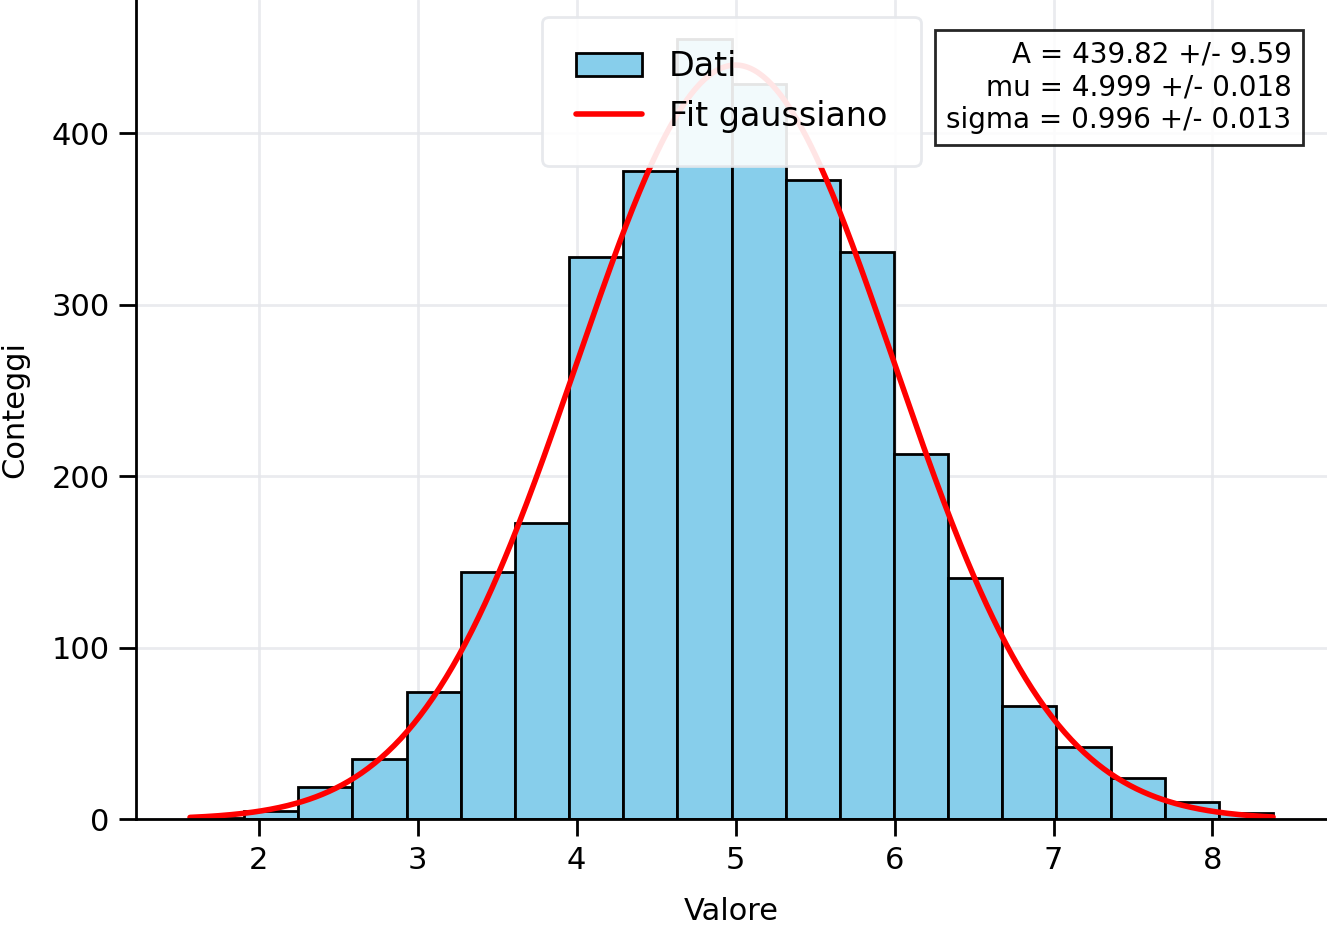
\includegraphics[width=0.82\textwidth]{fig_istogramma_fit.png}
\caption{Istogramma dei dati con sovrapposto il fit gaussiano.}
\label{fig:istogramma-fit}
\end{figure}

\subsection{Importazione di \texttt{curve\_fit}}

L'istruzione

\begin{lstlisting}[language=Python]
from scipy.optimize import curve_fit
\end{lstlisting}

importa la funzione di SciPy che determina i parametri ottimali del
modello.

\subsection{Definizione della funzione}

La funzione

\begin{lstlisting}[language=Python]
def gaussiana(x, A, mu, sigma):
    return A * np.exp(-(x - mu)**2 / (2 * sigma**2))
\end{lstlisting}

ha come primo argomento la variabile indipendente e, successivamente, i
parametri da determinare. Questa è la forma richiesta da
\texttt{curve\_fit}.

L'operazione \texttt{(x-mu)**2} è vettoriale: se \texttt{x} è un array,
NumPy calcola contemporaneamente il valore della gaussiana in tutti i
punti.

\subsection{Valori restituiti da \texttt{plt.hist}}

A differenza degli script precedenti, il risultato di \texttt{plt.hist}
non viene ignorato:

\begin{lstlisting}[language=Python]
conteggi, bin_edges, _ = plt.hist(...)
\end{lstlisting}

La funzione restituisce tre oggetti:

\begin{itemize}
    \item \texttt{conteggi}: numero di elementi in ogni bin;
    \item \texttt{bin\_edges}: bordi dei bin;
    \item il terzo oggetto contiene le barre grafiche; viene assegnato a
          \texttt{\_} perché non viene utilizzato.
\end{itemize}

Questa riga mostra chiaramente il doppio ruolo di \texttt{plt.hist}:
calcola l'istogramma e contemporaneamente lo disegna. Il fit successivo
usa \texttt{conteggi} e \texttt{bin\_edges}, non le barre grafiche.

\subsection{Calcolo dei centri dei bin}

Se i bordi sono

\[
b_0,b_1,\ldots,b_m,
\]

il centro del bin $i$ è

\[
x_i=\frac{b_i+b_{i+1}}{2}.
\]

In NumPy:

\begin{lstlisting}[language=Python]
bin_centri = (bin_edges[:-1] + bin_edges[1:]) / 2
\end{lstlisting}

L'espressione \texttt{bin\_edges[:-1]} contiene tutti i bordi tranne
l'ultimo; \texttt{bin\_edges[1:]} contiene tutti i bordi tranne il primo.
La somma elemento per elemento accoppia quindi il bordo sinistro e il
bordo destro di ciascun bin.

\subsection{Errori poissoniani e maschera}

Gli errori sono stimati mediante

\begin{lstlisting}[language=Python]
errori = np.sqrt(conteggi)
\end{lstlisting}

La riga

\begin{lstlisting}[language=Python]
errori[errori == 0] = 1
\end{lstlisting}

usa una maschera booleana. La condizione \texttt{errori == 0} seleziona
gli elementi nulli; l'assegnazione li sostituisce con 1. Ciò impedisce
che nel chi-quadro compaia una divisione per zero.

Una variante che esclude i bin vuoti è:

\begin{lstlisting}[language=Python]
maschera = conteggi > 0

centri_fit = bin_centri[maschera]
conteggi_fit = conteggi[maschera]
errori_fit = np.sqrt(conteggi[maschera])
\end{lstlisting}

In tal caso, i tre array filtrati devono essere passati a
\texttt{curve\_fit}.

\subsection{Stime iniziali}

La procedura di minimizzazione ha bisogno di valori iniziali:

\begin{lstlisting}[language=Python]
A0 = np.max(conteggi)
mu0 = np.mean(x)
sigma0 = np.std(x)
\end{lstlisting}

Le scelte sono naturali:

\begin{itemize}
    \item il massimo conteggio approssima l'altezza del picco;
    \item la media campionaria approssima il centro;
    \item la deviazione standard campionaria approssima la larghezza.
\end{itemize}

Questi valori vengono raccolti, nello stesso ordine degli argomenti della
funzione, in

\begin{lstlisting}[language=Python]
p0=[A0, mu0, sigma0]
\end{lstlisting}

\subsection{Esecuzione del fit}

La chiamata principale è

\begin{lstlisting}[language=Python]
popt, pcov = curve_fit(
    gaussiana,
    bin_centri,
    conteggi,
    p0=[A0, mu0, sigma0],
    sigma=errori,
    absolute_sigma=True
)
\end{lstlisting}

Gli argomenti indicano:

\begin{itemize}
    \item il modello da adattare;
    \item le ascisse dei punti, cioè i centri dei bin;
    \item le ordinate, cioè i conteggi;
    \item le stime iniziali dei parametri;
    \item le incertezze dei conteggi;
    \item l'interpretazione assoluta delle incertezze fornite.
\end{itemize}

L'array \texttt{popt} contiene i parametri ottimali:

\[
\texttt{popt}=[A,\mu,\sigma].
\]

La matrice \texttt{pcov} è la matrice di covarianza dei parametri.

\subsection{Matrice di covarianza e incertezze}

Per tre parametri, la matrice ha la forma

\[
\mathbf{C}=
\begin{pmatrix}
\operatorname{Var}(A) & \operatorname{Cov}(A,\mu) &
\operatorname{Cov}(A,\sigma)\\
\operatorname{Cov}(\mu,A) & \operatorname{Var}(\mu) &
\operatorname{Cov}(\mu,\sigma)\\
\operatorname{Cov}(\sigma,A) & \operatorname{Cov}(\sigma,\mu) &
\operatorname{Var}(\sigma)
\end{pmatrix}.
\]

Gli elementi diagonali sono le varianze dei parametri. Le incertezze
standard sono quindi

\[
\delta p_i=\sqrt{C_{ii}}.
\]

Nel codice:

\begin{lstlisting}[language=Python]
perr = np.sqrt(np.diag(pcov))
\end{lstlisting}

Gli elementi fuori diagonale descrivono invece le correlazioni tra le
stime dei parametri.

\subsection{Disegno di una curva regolare}

Il fit è stato eseguito nei centri dei bin, ma per disegnare una curva
regolare si genera una griglia più fitta:

\begin{lstlisting}[language=Python]
xfit = np.linspace(
    bin_edges[0],
    bin_edges[-1],
    500
)
\end{lstlisting}

La funzione gaussiana viene valutata nei 500 punti:

\begin{lstlisting}[language=Python]
yfit = gaussiana(xfit, *popt)
\end{lstlisting}

L'asterisco in \texttt{*popt} spacchetta l'array. L'istruzione equivale a

\begin{lstlisting}[language=Python]
yfit = gaussiana(
    xfit,
    popt[0],
    popt[1],
    popt[2]
)
\end{lstlisting}

La curva viene infine sovrapposta in rosso all'istogramma.

\subsection{Stampa dei risultati}

Le f-string

\begin{lstlisting}[language=Python]
print(f"A     = {popt[0]:.5g} +/- {perr[0]:.2g}")
print(f"mu    = {popt[1]:.5g} +/- {perr[1]:.2g}")
print(f"sigma = {popt[2]:.5g} +/- {perr[2]:.2g}")
\end{lstlisting}

stampano cinque cifre significative per i parametri e due per le
incertezze. Nello script Python originale il simbolo \texttt{+/-} può
essere sostituito dal carattere Unicode \texttt{±}, se il terminale e il
file sorgente usano una codifica compatibile.

\section{Osservazioni statistiche}

Il fit presentato è un fit ai conteggi raggruppati. La scelta dei bin
influenza sia le ascisse del fit sia i conteggi. Due istogrammi costruiti
con numeri di bin differenti possono quindi produrre parametri
leggermente differenti.

L'approssimazione $\sqrt{N_i}$ è più affidabile quando i conteggi non
sono troppo piccoli. Per conteggi bassi o numerosi bin vuoti, una
trattazione poissoniana basata sulla verosimiglianza è in genere più
adeguata del chi-quadro gaussiano. Nel contesto didattico corrente,
questa procedura permette comunque di collegare in modo trasparente:

\begin{center}
\texttt{dati grezzi}
$\longrightarrow$
\texttt{istogramma}
$\longrightarrow$
\texttt{conteggi e centri}
$\longrightarrow$
\texttt{fit gaussiano}.
\end{center}

\section{Riepilogo}

Il percorso seguito mostra progressivamente che:

\begin{enumerate}
    \item un istogramma è innanzitutto un algoritmo di conteggio;
    \item \texttt{plt.hist} calcola i conteggi e disegna le barre;
    \item \texttt{bins} controlla la suddivisione dell'intervallo;
    \item i valori restituiti da \texttt{plt.hist} possono essere usati
          in calcoli successivi;
    \item il fit non usa direttamente gli oggetti grafici, ma i centri e
          i conteggi dei bin;
    \item \texttt{curve\_fit} restituisce i parametri ottimali e la loro
          matrice di covarianza;
    \item la diagonale della matrice di covarianza permette di ricavare
          le incertezze sui parametri.
\end{enumerate}




\chapter{Machere in numpy}
Una delle caratteristiche più utili di NumPy è la possibilità di selezionare e modificare contemporaneamente più elementi di un array mediante una \emph{maschera booleana}.

\section{Machere in numpy}
Una maschera booleana è un array che contiene esclusivamente i valori logici \texttt{True} e \texttt{False}. In genere, la maschera ha la stessa dimensione dell'array sul quale deve essere applicata:

\begin{itemize}
    \item \texttt{True} indica che l'elemento deve essere selezionato;
    \item \texttt{False} indica che l'elemento non deve essere selezionato.
\end{itemize}

Le maschere consentono di evitare molti cicli \texttt{for} espliciti e permettono di scrivere operazioni compatte, leggibili ed efficienti.

Consideriamo il seguente array:

\begin{lstlisting}
import numpy as np

x = np.array([3, 7, 2, 9, 5])
\end{lstlisting}

Vogliamo individuare gli elementi maggiori di 5. Possiamo scrivere:

\begin{lstlisting}
maschera = x > 5
print(maschera)
\end{lstlisting}

Il risultato è:

\begin{lstlisting}
[False  True False  True False]
\end{lstlisting}

NumPy esegue il confronto elemento per elemento:

\begin{center}
\begin{tabular}{ccc}
\toprule
Elemento & Condizione & Risultato \\
\midrule
3 & $3>5$ & \texttt{False} \\
7 & $7>5$ & \texttt{True} \\
2 & $2>5$ & \texttt{False} \\
9 & $9>5$ & \texttt{True} \\
5 & $5>5$ & \texttt{False} \\
\bottomrule
\end{tabular}
\end{center}

\section{Selezione degli elementi}

La maschera può essere inserita tra parentesi quadre per estrarre gli elementi corrispondenti ai valori \texttt{True}:

\begin{lstlisting}
selezionati = x[maschera]
print(selezionati)
\end{lstlisting}

Il risultato è:

\begin{lstlisting}
[7 9]
\end{lstlisting}

La stessa operazione può essere scritta in forma compatta:

\begin{lstlisting}
selezionati = x[x > 5]
\end{lstlisting}

Questa istruzione non modifica \texttt{x}: crea un nuovo array contenente soltanto gli elementi selezionati.

\section{Modifica degli elementi selezionati}

Una maschera può essere utilizzata anche a sinistra dell'operatore di assegnazione. In questo caso gli elementi selezionati vengono modificati direttamente:

\begin{lstlisting}
x = np.array([3, 7, 2, 9, 5])

x[x > 5] = 0

print(x)
\end{lstlisting}

Il risultato è:

\begin{lstlisting}
[3 0 2 0 5]
\end{lstlisting}

Tutti gli elementi maggiori di 5 sono stati sostituiti con zero.

È importante distinguere le due operazioni:

\begin{lstlisting}
y = x[x > 5]     # seleziona e crea un nuovo array
x[x > 5] = 0     # modifica direttamente l'array x
\end{lstlisting}

\section{Esempio: sostituire i valori negativi}

Consideriamo un array contenente valori positivi e negativi:

\begin{lstlisting}
x = np.array([5, -2, 3, -7, 8])
\end{lstlisting}

Per sostituire tutti i valori negativi con zero:

\begin{lstlisting}
x[x < 0] = 0
print(x)
\end{lstlisting}

Si ottiene:

\begin{lstlisting}
[5 0 3 0 8]
\end{lstlisting}

L'istruzione equivale concettualmente al seguente ciclo:

\begin{lstlisting}
for i in range(len(x)):
    if x[i] < 0:
        x[i] = 0
\end{lstlisting}

La versione con la maschera è però più compatta e più vicina allo stile di programmazione vettoriale di NumPy.

\section{Il caso degli errori dell'istogramma}

Nel fit di un istogramma si può stimare l'incertezza statistica di ciascun conteggio mediante:

\[
\sigma_i = \sqrt{N_i},
\]

dove $N_i$ è il numero di eventi contenuti nel bin $i$.

In Python:

\begin{lstlisting}
conteggi = np.array([25, 9, 0, 16, 0])
errori = np.sqrt(conteggi)

print(errori)
\end{lstlisting}

Il risultato è:

\begin{lstlisting}
[5. 3. 0. 4. 0.]
\end{lstlisting}

I bin vuoti hanno conteggio nullo e quindi errore nullo. Per evitare una divisione per zero in un fit pesato, si può scrivere:

\begin{lstlisting}
errori[errori == 0] = 1
\end{lstlisting}

La condizione

\begin{lstlisting}
errori == 0
\end{lstlisting}

produce la maschera:

\begin{lstlisting}
[False False True False True]
\end{lstlisting}

L'assegnazione sostituisce con 1 soltanto gli elementi corrispondenti ai valori \texttt{True}:

\begin{lstlisting}
[5. 3. 1. 4. 1.]
\end{lstlisting}

Questa soluzione evita la divisione per zero, ma attribuisce convenzionalmente errore 1 ai bin vuoti.

\section{Escludere i bin vuoti dal fit}

In molti casi è preferibile non modificare gli errori, ma escludere dal fit i bin con conteggio nullo:

\begin{lstlisting}
maschera = conteggi > 0

conteggi_fit = conteggi[maschera]
centri_fit = centri[maschera]
errori_fit = np.sqrt(conteggi[maschera])
\end{lstlisting}

La stessa maschera deve essere applicata a tutti gli array associati agli stessi punti sperimentali. In questo modo, i conteggi, i centri dei bin e gli errori continuano ad avere la stessa lunghezza e a riferirsi agli stessi bin.

Nel fit gaussiano si può quindi scrivere:

\begin{lstlisting}
maschera = conteggi > 0

popt, pcov = curve_fit(
    gaussiana,
    centri[maschera],
    conteggi[maschera],
    sigma=np.sqrt(conteggi[maschera]),
    absolute_sigma=True
)
\end{lstlisting}

\section{Condizioni multiple}

Le maschere possono combinare più condizioni.

\subsection{Operatore logico AND}

Per selezionare i valori compresi tra 0 e 10, estremi inclusi:

\begin{lstlisting}
maschera = (x >= 0) & (x <= 10)
selezionati = x[maschera]
\end{lstlisting}

L'operatore \texttt{\&} richiede che entrambe le condizioni siano vere.

\subsection{Operatore logico OR}

Per selezionare i valori minori di 0 oppure maggiori di 10:

\begin{lstlisting}
maschera = (x < 0) | (x > 10)
\end{lstlisting}

L'operatore \texttt{|} richiede che almeno una delle condizioni sia vera.

\subsection{Negazione}

Per invertire una maschera si usa \texttt{\textasciitilde}:

\begin{lstlisting}
maschera = x > 5
maschera_inversa = ~maschera
\end{lstlisting}

La maschera inversa seleziona gli elementi che non soddisfano la condizione originale.

\subsection{Importanza delle parentesi}

Ogni confronto deve essere racchiuso tra parentesi:

\begin{lstlisting}
maschera = (x >= 0) & (x <= 10)
\end{lstlisting}

Non si devono usare \texttt{and}, \texttt{or} e \texttt{not}, perché questi operatori sono progettati per singoli valori logici, non per array NumPy.

\section{Maschere con valori non validi}

In un'analisi numerica può essere necessario eliminare valori \texttt{NaN} o infiniti. NumPy fornisce la funzione \texttt{isfinite}:

\begin{lstlisting}
x = np.array([1.0, np.nan, 3.0, np.inf, 5.0])

maschera = np.isfinite(x)
x_valido = x[maschera]

print(x_valido)
\end{lstlisting}

Il risultato è:

\begin{lstlisting}
[1. 3. 5.]
\end{lstlisting}

Per sostituire i valori non finiti con zero:

\begin{lstlisting}
x[~np.isfinite(x)] = 0
\end{lstlisting}

\section{Uso di \texttt{np.where}}

Quando si vuole scegliere tra due valori senza eliminare elementi, si può utilizzare \texttt{np.where}:

\begin{lstlisting}
x = np.array([-3, 4, -1, 7, 2])

y = np.where(x < 0, 0, x)

print(y)
\end{lstlisting}

Il risultato è:

\begin{lstlisting}
[0 4 0 7 2]
\end{lstlisting}

L'istruzione significa:

\begin{quote}
se la condizione \texttt{x < 0} è vera, usa 0; altrimenti usa il valore di \texttt{x}.
\end{quote}

A differenza di

\begin{lstlisting}
x[x < 0] = 0
\end{lstlisting}

\texttt{np.where} crea un nuovo array e lascia invariato l'array originale, salvo una successiva riassegnazione.

\section{Errori comuni}

\subsection{Usare una lista Python al posto di un array NumPy}

Le maschere booleane nella forma descritta richiedono array NumPy:

\begin{lstlisting}
x = [1, 2, 3, 4]
# x[x > 2] non funziona: x e una lista Python
\end{lstlisting}

Occorre prima convertire la lista:

\begin{lstlisting}
x = np.array(x)
y = x[x > 2]
\end{lstlisting}

\subsection{Applicare maschere differenti ad array collegati}

Se \texttt{x} e \texttt{y} descrivono gli stessi punti, bisogna applicare la stessa maschera:

\begin{lstlisting}
maschera = y > 0

x_fit = x[maschera]
y_fit = y[maschera]
\end{lstlisting}

Applicare condizioni diverse può distruggere la corrispondenza tra le coordinate.

\subsection{Confondere selezione e modifica}

L'istruzione

\begin{lstlisting}
y = x[x > 0]
\end{lstlisting}

seleziona gli elementi e crea \texttt{y}. L'istruzione

\begin{lstlisting}
x[x > 0] = 1
\end{lstlisting}

modifica invece gli elementi selezionati nell'array originale.

\section{Esercizi}

\subsection*{Esercizio 1: selezione di valori positivi}

Dato l'array

\begin{lstlisting}
x = np.array([-4, 7, -2, 0, 5, 9, -1])
\end{lstlisting}

costruire una maschera che selezioni soltanto i valori strettamente positivi e stampare il nuovo array.

\subsection*{Esercizio 2: sostituzione dei valori negativi}

Usando lo stesso array dell'esercizio precedente, sostituire tutti i valori negativi con zero senza utilizzare un ciclo \texttt{for}.

\subsection*{Esercizio 3: selezione in un intervallo}

Dato

\begin{lstlisting}
x = np.array([-3, 1, 4, 7, 10, 12, 15])
\end{lstlisting}

selezionare tutti i valori compresi tra 4 e 12, estremi inclusi.

\subsection*{Esercizio 4: valori esterni a un intervallo}

Con lo stesso array, selezionare i valori minori di 4 oppure maggiori di 12.

\subsection*{Esercizio 5: numeri pari}

Dato

\begin{lstlisting}
x = np.array([1, 2, 3, 4, 5, 6, 7, 8])
\end{lstlisting}

costruire una maschera che selezioni soltanto i numeri pari. Si ricorda che il resto della divisione per 2 si calcola con l'operatore \texttt{\%}.

\subsection*{Esercizio 6: modifica condizionata}

Nell'array

\begin{lstlisting}
x = np.array([2, 5, 8, 11, 14, 17])
\end{lstlisting}

sostituire con il valore 100 tutti gli elementi maggiori di 10.

\subsection*{Esercizio 7: filtraggio coordinato}

Sono date due misure associate:

\begin{lstlisting}
x = np.array([0, 1, 2, 3, 4, 5])
y = np.array([2.1, -1.0, 4.3, 0.0, 5.2, -0.5])
\end{lstlisting}

selezionare i punti per i quali $y>0$, applicando la stessa maschera sia a \texttt{x} sia a \texttt{y}.

\subsection*{Esercizio 8: dati non validi}

Dato

\begin{lstlisting}
x = np.array([1.2, np.nan, 3.4, np.inf, -2.0, 5.1])
\end{lstlisting}

creare un nuovo array contenente soltanto i valori finiti.

\subsection*{Esercizio 9: errori poissoniani}

Dato l'array dei conteggi

\begin{lstlisting}
conteggi = np.array([16, 0, 25, 9, 0, 36])
\end{lstlisting}

calcolare gli errori $\sqrt{N}$ e sostituire gli errori nulli con 1 mediante una maschera.

\subsection*{Esercizio 10: esclusione dei bin vuoti}

Usando i conteggi dell'esercizio precedente e

\begin{lstlisting}
centri = np.array([0.5, 1.5, 2.5, 3.5, 4.5, 5.5])
\end{lstlisting}

costruire gli array \texttt{conteggi\_fit}, \texttt{centri\_fit} ed \texttt{errori\_fit}, escludendo i bin vuoti.

\subsection*{Esercizio 11: selezione combinata}

Dato

\begin{lstlisting}
x = np.array([-5, -1, 0, 3, 8, 11, 15])
\end{lstlisting}

selezionare i valori non negativi e strettamente minori di 10.

\subsection*{Esercizio 12: uso di \texttt{np.where}}

Dato

\begin{lstlisting}
x = np.array([-3, 4, -1, 7, 2])
\end{lstlisting}

creare un nuovo array nel quale i valori negativi siano sostituiti con il loro valore assoluto, lasciando invariati quelli positivi.

\section{Soluzioni degli esercizi}

\subsection*{Soluzione 1}

\begin{lstlisting}
maschera = x > 0
positivi = x[maschera]
print(positivi)
\end{lstlisting}

\subsection*{Soluzione 2}

\begin{lstlisting}
x[x < 0] = 0
print(x)
\end{lstlisting}

\subsection*{Soluzione 3}

\begin{lstlisting}
maschera = (x >= 4) & (x <= 12)
print(x[maschera])
\end{lstlisting}

\subsection*{Soluzione 4}

\begin{lstlisting}
maschera = (x < 4) | (x > 12)
print(x[maschera])
\end{lstlisting}

\subsection*{Soluzione 5}

\begin{lstlisting}
maschera = x % 2 == 0
pari = x[maschera]
print(pari)
\end{lstlisting}

\subsection*{Soluzione 6}

\begin{lstlisting}
x[x > 10] = 100
print(x)
\end{lstlisting}

\subsection*{Soluzione 7}

\begin{lstlisting}
maschera = y > 0

x_selezionato = x[maschera]
y_selezionato = y[maschera]

print(x_selezionato)
print(y_selezionato)
\end{lstlisting}

\subsection*{Soluzione 8}

\begin{lstlisting}
maschera = np.isfinite(x)
x_valido = x[maschera]
print(x_valido)
\end{lstlisting}

\subsection*{Soluzione 9}

\begin{lstlisting}
errori = np.sqrt(conteggi)
errori[errori == 0] = 1
print(errori)
\end{lstlisting}

\subsection*{Soluzione 10}

\begin{lstlisting}
maschera = conteggi > 0

conteggi_fit = conteggi[maschera]
centri_fit = centri[maschera]
errori_fit = np.sqrt(conteggi[maschera])

print(conteggi_fit)
print(centri_fit)
print(errori_fit)
\end{lstlisting}

\subsection*{Soluzione 11}

\begin{lstlisting}
maschera = (x >= 0) & (x < 10)
print(x[maschera])
\end{lstlisting}

\subsection*{Soluzione 12}

\begin{lstlisting}
y = np.where(x < 0, -x, x)
print(y)
\end{lstlisting}

\section{Conclusioni}

Le maschere booleane consentono di:

\begin{itemize}
    \item selezionare elementi che soddisfano una condizione;
    \item modificare contemporaneamente gruppi di elementi;
    \item filtrare dati sperimentali non validi;
    \item applicare lo stesso criterio a più array associati;
    \item preparare dati, conteggi ed errori per un fit;
    \item sostituire molti cicli \texttt{for} con operazioni vettoriali.
\end{itemize}

La forma generale per selezionare è:

\begin{lstlisting}
selezionati = array[condizione]
\end{lstlisting}

La forma generale per modificare è:

\begin{lstlisting}
array[condizione] = nuovo_valore
\end{lstlisting}

Queste due istruzioni costituiscono la base dell'uso delle maschere booleane in NumPy.


\chapter{Il mondo della sottrazione del fondo}
Questa lezione propone un percorso unitario per comprendere il fit di una distribuzione composta da due segnali gaussiani sovrapposti a un fondo parabolico. Il percorso parte dal fit globale, prosegue con la sottrazione del fondo e la corretta propagazione delle incertezze, introduce residui e pull e conduce infine alla costruzione del $\chi^2$, del $\chi^2$ ridotto e del $p$-value. L'obiettivo non è soltanto applicare formule, ma mostrare che residui, pull e $\chi^2$ sono livelli successivi della stessa analisi statistica.


\section{Obiettivi didattici}
Al termine dell'attività lo studente dovrebbe essere in grado di:
\begin{itemize}
  \item modellizzare una distribuzione composta da due gaussiane e da un fondo parabolico;
  \item eseguire un fit globale e interpretarne i parametri e la matrice di covarianza;
  \item sottrarre il fondo senza attribuire ai dati puliti incertezze statistiche non corrette;
  \item costruire e interpretare residui e pull;
  \item riconoscere il pull al quadrato come contributo del singolo punto al $\chi^2$;
  \item calcolare $\chi^2$, numero di gradi di libertà, $\chi^2$ ridotto e $p$-value;
  \item diagnosticare bias, errori sovrastimati o sottostimati e inadeguatezza del modello.
\end{itemize}

\section{Il problema: due gaussiane su un fondo parabolico}
Consideriamo una distribuzione descritta dal modello
\begin{equation}
  f(x;\bm\theta)=G_1(x)+G_2(x)+B(x),
\end{equation}
dove
\begin{align}
  G_j(x) &= A_j\exp\!\left[-\frac{(x-\mu_j)^2}{2\sigma_j^2}\right], \qquad j=1,2,\\
  B(x) &= a+bx+cx^2.
\end{align}
Il vettore completo dei parametri può essere scritto come
\begin{equation}
 \bm\theta=(A_1,\mu_1,\sigma_1,A_2,\mu_2,\sigma_2,a,b,c).
\end{equation}

Il primo obiettivo è effettuare un fit globale, determinando simultaneamente i parametri dei due segnali e quelli del fondo. La sovrapposizione tra picchi e fondo rende il problema interessante: i parametri non sono generalmente indipendenti e le loro correlazioni sono contenute nella matrice di covarianza restituita dal fit.

\begin{figure}[htbp]
  \centering
  \fbox{\parbox[c][5.5cm][c]{0.86\textwidth}{\centering Inserire qui la figura dei dati con il fit globale, le due componenti gaussiane e il fondo parabolico.}}
  \caption{Fit globale della distribuzione composta da due gaussiane e da un fondo parabolico.}
  \label{fig:fitglobale}
\end{figure}

\section{Sottrazione del fondo e corretta propagazione dell'errore}
\subsection{Valore centrale dei dati puliti}
Indichiamo con $y_i$ il contenuto del bin $i$ e con $B_i$ il fondo stimato nello stesso bin. Il dato dopo la sottrazione del fondo è
\begin{equation}
  y_i^{\mathrm{clean}}=y_i-B_i.
\end{equation}
Nel caso di un modello continuo confrontato con conteggi per bin, $B_i$ dovrebbe essere il valore atteso integrato sull'intervallo del bin, oppure un'approssimazione coerente con quella impiegata nel fit.

\subsection{L'errore concettuale da evitare}
Sarebbe errato trattare $y_i^{\mathrm{clean}}$ come se fosse un nuovo campione acquisito in assenza di fondo e assegnargli automaticamente
\begin{equation}
  \sigma_{i,\mathrm{clean}}=\sqrt{y_i^{\mathrm{clean}}}.
\end{equation}
La sottrazione modifica il valore centrale, ma non cancella le fluttuazioni statistiche prodotte dagli eventi di fondo presenti nella misura originale. Inoltre, $y_i^{\mathrm{clean}}$ può essere piccolo o persino negativo, mentre la sua incertezza deve rimanere ben definita. Questo passaggio permette di distinguere tra \emph{rimozione della stima del fondo} e \emph{rimozione delle sue fluttuazioni}, che non avviene mediante una semplice sottrazione.

Se $y_i$ è un conteggio poissoniano e il fondo fosse noto esattamente, una stima elementare sarebbe
\begin{equation}
  \mathrm{Var}(y_i^{\mathrm{clean}})=\mathrm{Var}(y_i)\simeq y_i,
  \qquad
  \sigma_{i,\mathrm{clean}}\simeq\sqrt{y_i},
\end{equation}
non $\sqrt{y_i-B_i}$.

\subsection{Incertezza del fondo dalla matrice di covarianza del fit}
Siano
\begin{equation}
  \bm\beta=(a,b,c)
\end{equation}
i parametri del fondo e $\mathbf C_{\beta}$ la loro matrice di covarianza. Per
\begin{equation}
 B_i=B(x_i;\bm\beta)=a+b x_i+c x_i^2,
\end{equation}
il gradiente rispetto ai parametri è
\begin{equation}
  \mathbf J_i=\left(\frac{\partial B_i}{\partial a},
  \frac{\partial B_i}{\partial b},
  \frac{\partial B_i}{\partial c}\right)
  =(1,x_i,x_i^2).
\end{equation}
L'incertezza propagata sul fondo vale quindi
\begin{equation}
  \mathrm{Var}(B_i)=\mathbf J_i\,\mathbf C_{\beta}\,\mathbf J_i^{T}.
\end{equation}
In forma esplicita,
\begin{align}
 \mathrm{Var}(B_i)={}&C_{aa}+x_i^2C_{bb}+x_i^4C_{cc}
 +2x_iC_{ab}+2x_i^2C_{ac}+2x_i^3C_{bc}.
\end{align}
I termini fuori diagonale non devono essere eliminati: rappresentano le covarianze tra i parametri del fondo e possono aumentare o diminuire l'incertezza propagata.

\subsection{Errore sui dati puliti}
La formula generale è
\begin{equation}
 \boxed{
 \mathrm{Var}(y_i^{\mathrm{clean}})
 =\mathrm{Var}(y_i)+\mathrm{Var}(B_i)
 -2\,\mathrm{Cov}(y_i,B_i)
 }
 \label{eq:varclean}
\end{equation}
Se la stima del fondo proviene da un campione indipendente, oppure si assume trascurabile la correlazione con $y_i$, si usa l'approssimazione
\begin{equation}
 \boxed{
 \sigma_{i,\mathrm{clean}}^2
 \simeq \sigma_{y_i}^2+
 \mathbf J_i\mathbf C_{\beta}\mathbf J_i^T
 }.
 \label{eq:varcleanapprox}
\end{equation}
Per conteggi poissoniani, $\sigma_{y_i}^2\simeq y_i$.

Quando invece il fondo è ottenuto dallo stesso fit eseguito sugli stessi dati, $y_i$ e $B_i$ non sono strettamente indipendenti. In tal caso il termine incrociato di Eq.~\eqref{eq:varclean} non è automaticamente nullo. La sola somma in quadratura di Eq.~\eqref{eq:varcleanapprox} è allora un'approssimazione, utile didatticamente ma da dichiarare. Una trattazione completa richiede la covarianza tra osservazione e previsione, oppure una procedura di replica, come simulazioni Monte Carlo o bootstrap, che ripeta il fit e la sottrazione del fondo.

Più in generale, i valori del fondo stimati in bin diversi sono correlati:
\begin{equation}
 \mathrm{Cov}(B_i,B_j)=\mathbf J_i\mathbf C_{\beta}\mathbf J_j^T.
\end{equation}
La sottrazione del fondo può quindi produrre una matrice di covarianza non diagonale per l'intero vettore dei dati puliti. Se queste correlazioni sono rilevanti, il confronto successivo deve usare il $\chi^2$ matriciale:
\begin{equation}
 \chi^2=\mathbf r^T\mathbf V^{-1}\mathbf r,
\end{equation}
dove $\mathbf V$ è la matrice di covarianza dei dati analizzati.

\begin{figure}[htbp]
  \centering
  \fbox{\parbox[c][5.5cm][c]{0.86\textwidth}{\centering Inserire qui la figura dei dati dopo la sottrazione del fondo, con barre di errore correttamente propagate.}}
  \caption{Distribuzione dopo la sottrazione del fondo. Le incertezze non sono ottenute come radice quadrata dei contenuti sottratti.}
  \label{fig:clean}
\end{figure}

\section{Residui}
Per ogni punto o bin definiamo il residuo
\begin{equation}
 r_i=y_i-f(x_i;\widehat{\bm\theta}).
\end{equation}
I residui dovrebbero oscillare in modo non strutturato attorno allo zero. Sequenze di residui dello stesso segno, curvature o variazioni sistematiche possono rivelare un modello inadeguato anche quando un singolo indicatore numerico appare accettabile.

\begin{figure}[htbp]
  \centering
  \fbox{\parbox[c][4.8cm][c]{0.86\textwidth}{\centering Inserire qui il grafico dei residui in funzione di $x$.}}
  \caption{Residui del fit.}
  \label{fig:residui}
\end{figure}

\section{Pull e loro distribuzione}
Il pull del punto $i$ è il residuo normalizzato alla sua incertezza:
\begin{equation}
 p_i=\frac{y_i-f(x_i;\widehat{\bm\theta})}{\sigma_i}.
\end{equation}
In presenza di covarianze tra i punti, questa definizione punto per punto è soltanto una rappresentazione diagnostica semplificata. Una normalizzazione rigorosa richiede residui decorrelati, ottenibili per esempio mediante una fattorizzazione della matrice $\mathbf V$.

Se il modello è corretto, le incertezze sono stimate adeguatamente e le approssimazioni gaussiane sono valide, la distribuzione dei pull dovrebbe essere approssimativamente normale con
\begin{equation}
 \mu_{\mathrm{pull}}\simeq0,
 \qquad
 \sigma_{\mathrm{pull}}\simeq1.
\end{equation}
L'interpretazione è la seguente:
\begin{itemize}
 \item $\mu_{\mathrm{pull}}\neq0$: possibile bias sistematico;
 \item $\sigma_{\mathrm{pull}}>1$: dispersione maggiore di quella prevista, errori sottostimati o modello incompleto;
 \item $\sigma_{\mathrm{pull}}<1$: dispersione minore di quella prevista, errori sovrastimati o correlazioni non considerate.
\end{itemize}
Media e larghezza dei pull sono strumenti diagnostici, non sostituiscono da sole un test di bontà del fit. Inoltre, i pull ottenuti dagli stessi dati impiegati per stimare i parametri non sono in generale perfettamente indipendenti.

\begin{figure}[htbp]
  \centering
  \begin{subfigure}{0.48\textwidth}
    \centering
    \fbox{\parbox[c][4.5cm][c]{0.9\textwidth}{\centering Pull in funzione di $x$.}}
    \caption{Pull per ogni bin.}
  \end{subfigure}
  \hfill
  \begin{subfigure}{0.48\textwidth}
    \centering
    \fbox{\parbox[c][4.5cm][c]{0.9\textwidth}{\centering Istogramma dei pull con fit gaussiano.}}
    \caption{Distribuzione dei pull.}
  \end{subfigure}
  \caption{Analisi dei pull.}
  \label{fig:pull}
\end{figure}

\section{Dal pull al $\chi^2$}
Elevando al quadrato il pull si ottiene
\begin{equation}
 p_i^2=\frac{[y_i-f(x_i;\widehat{\bm\theta})]^2}{\sigma_i^2}.
\end{equation}
Questa quantità rappresenta, nel caso di errori indipendenti, il contributo del singolo punto al $\chi^2$:
\begin{equation}
 \chi_i^2=p_i^2.
\end{equation}
La somma dei contributi fornisce
\begin{equation}
 \boxed{
 \chi^2=\sum_{i=1}^{N}p_i^2
 =\sum_{i=1}^{N}
 \frac{[y_i-f(x_i;\widehat{\bm\theta})]^2}{\sigma_i^2}
 }.
\end{equation}
Questo realizza il percorso concettuale
\begin{center}
 dato $\longrightarrow$ residuo $\longrightarrow$ pull $\longrightarrow$ pull$^2$
 $\longrightarrow$ somma $\longrightarrow\chi^2$.
\end{center}

\subsection{Somma cumulativa dei contributi}
Definiamo
\begin{equation}
 C_k=\sum_{i=1}^{k}p_i^2.
\end{equation}
Il valore finale è
\begin{equation}
 C_N=\chi^2.
\end{equation}
Il grafico di $C_k$ mostra come il $\chi^2$ osservato si costruisca punto dopo punto e permette di individuare regioni che producono incrementi particolarmente grandi.

È importante non confondere $C_k$ con la funzione di ripartizione della distribuzione teorica del $\chi^2$. La prima è una somma progressiva dei contributi osservati; la seconda è una probabilità teorica associata a una variabile casuale $\chi^2$ con un determinato numero di gradi di libertà.

\begin{figure}[htbp]
  \centering
  \begin{subfigure}{0.48\textwidth}
    \centering
    \fbox{\parbox[c][4.5cm][c]{0.9\textwidth}{\centering Contributi $p_i^2$ per bin.}}
    \caption{Contributi individuali.}
  \end{subfigure}
  \hfill
  \begin{subfigure}{0.48\textwidth}
    \centering
    \fbox{\parbox[c][4.5cm][c]{0.9\textwidth}{\centering Somma cumulativa $C_k$.}}
    \caption{Costruzione progressiva del $\chi^2$.}
  \end{subfigure}
  \caption{Dal pull al $\chi^2$.}
  \label{fig:chi2build}
\end{figure}

\section{Gradi di libertà, $\chi^2$ ridotto e $p$-value}
Se si hanno $N$ osservazioni indipendenti e si stimano $m$ parametri liberi, il numero di gradi di libertà è, nelle condizioni usuali,
\begin{equation}
 \nu=N-m.
\end{equation}
Si definisce quindi
\begin{equation}
 \chi^2_{\mathrm{rid}}=\frac{\chi^2}{\nu}.
\end{equation}
Un valore prossimo a uno è spesso compatibile con un modello e con una stima degli errori ragionevoli, ma non costituisce da solo una prova di correttezza. Occorre considerare $\nu$, osservare i residui e valutare il $p$-value.

La funzione di ripartizione teorica è
\begin{equation}
 F_{\chi^2_\nu}(q)=P(\chi^2_\nu\le q),
\end{equation}
mentre il $p$-value per la coda superiore è
\begin{equation}
 p=P(\chi^2_\nu\ge\chi^2_{\mathrm{obs}})
 =1-F_{\chi^2_\nu}(\chi^2_{\mathrm{obs}}).
\end{equation}
Esso quantifica quanto sia estremo il valore osservato sotto le ipotesi del modello e del modello d'errore adottati. Non misura la probabilità che il modello sia vero.

\begin{figure}[htbp]
  \centering
  \fbox{\parbox[c][5.5cm][c]{0.86\textwidth}{\centering Inserire qui la distribuzione teorica $\chi^2_\nu$, il valore osservato e l'area di coda corrispondente al $p$-value.}}
  \caption{Distribuzione teorica del $\chi^2$ e interpretazione del $p$-value.}
  \label{fig:pvalue}
\end{figure}

\section{Sequenza operativa dell'esercitazione}
\begin{enumerate}[label=\arabic*.]
 \item Generare o caricare una distribuzione con due gaussiane e un fondo parabolico.
 \item Costruire l'istogramma, conservando conteggi, bordi e centri dei bin.
 \item Eseguire il fit globale e riportare parametri, errori e matrice di covarianza.
 \item Visualizzare separatamente le due gaussiane, il fondo e la funzione totale.
 \item Calcolare il fondo atteso in ogni bin e sottrarlo ai dati.
 \item Propagare l'incertezza del fondo con $\mathbf J_i\mathbf C_{\beta}\mathbf J_i^T$, includendo i termini di covarianza.
 \item Dichiarare se il fondo è indipendente dai dati o stimato sugli stessi dati; nel secondo caso discutere il termine $-2\,\mathrm{Cov}(y_i,B_i)$.
 \item Fittare o confrontare la distribuzione pulita con il modello dei soli segnali.
 \item Calcolare e rappresentare i residui.
 \item Calcolare i pull e fittarne l'istogramma con una gaussiana.
 \item Interpretare $\mu_{\mathrm{pull}}$ e $\sigma_{\mathrm{pull}}$.
 \item Calcolare $p_i^2$, i contributi al $\chi^2$ e la loro somma cumulativa.
 \item Determinare $\chi^2$, $\nu$, $\chi^2/\nu$ e $p$-value.
 \item Confrontare le conclusioni ottenute da residui, pull e test del $\chi^2$.
\end{enumerate}

\section{Seconda fase: codici e figure a corredo della lezione}
La naturale prosecuzione consiste nell'implementare l'intero percorso in script Python riproducibili. Gli script possono essere forniti come materiale complementare, mentre le figure da essi prodotte vengono integrate nei punti corrispondenti della lezione.

Una struttura consigliata è:
\begin{description}
 \item[\texttt{01\_genera\_dati.py}] generazione del campione e salvataggio dei dati;
 \item[\texttt{02\_fit\_globale.py}] istogramma, modello completo, fit e matrice di covarianza;
 \item[\texttt{03\_sottrai\_fondo.py}] sottrazione del fondo e propagazione delle incertezze;
 \item[\texttt{04\_residui\_pull.py}] residui, pull e fit gaussiano della distribuzione dei pull;
 \item[\texttt{05\_chi2.py}] contributi $p_i^2$, somma cumulativa, $\chi^2$ ridotto e $p$-value;
 \item[\texttt{06\_studio\_toyMC.py}] studio opzionale con molti pseudo-esperimenti per verificare le distribuzioni attese.
\end{description}

Per rendere il materiale riproducibile, ogni script dovrebbe:
\begin{itemize}
 \item fissare o registrare il seme del generatore casuale;
 \item salvare le figure in formato PDF, ed eventualmente PNG per l'anteprima;
 \item stampare in modo ordinato parametri, incertezze, covarianze, $\chi^2$, gradi di libertà e $p$-value;
 \item usare nomi di file coerenti con le etichette delle figure nel documento;
 \item separare la generazione dei dati dall'analisi, così che gli studenti possano lavorare anche su un campione già fornito.
\end{itemize}

\section{Osservazione metodologica conclusiva}
Il valore didattico dell'attività consiste nel non presentare fit, sottrazione del fondo, residui, pull e $\chi^2$ come argomenti indipendenti. Essi formano una catena logica unica. Il punto più delicato è la gestione delle incertezze: sottrarre un fondo non equivale ad avere acquisito dati senza fondo, e la covarianza dei parametri del modello deve essere propagata. La fase successiva, con codici e figure, renderà visibile ogni passaggio e permetterà agli studenti di verificare direttamente le conseguenze di ipotesi corrette o scorrette sugli errori.

\appendix
\section{Segnaposto per i materiali allegati}
Gli script completi saranno inseri

\end{document}
